
\documentclass[spanish,openright]{book}

%%%%%%%%%%%%%%%%%%%%%%%%%%%%%%%%%%%%%%%%%%%%%%%%%%%%%%%%%%%%%%%%%%%%%%%%%%%
% Comienzo del Preamble y seccion de configuracion
%

%% FIXING PROBLEM WITH ALL PAGES PRINTED IN COLOR \documentclass[RGB,rgb,svgnames,spanish,openright]{book}
%\documentclass[spanish,openright]{book}
% \documentclass[english,openright]{book}
% \documentclass[11pt,english,twoside,openright]{book}

% \usepackage[a4,cam,center]{crop}
% \crop[font=\upshape\mdseries\small\textsf]

\synctex=1

% ifthen to allow using language dependent settings
\usepackage{ifthen}

%% JMG: FIXING PROBLEM WITH ALL PAGES PRINTED IN COLOR
% This should not be touched, as it should work as it is know.
\newcommand{\colorspaceused}{rgb}

%The next section seems to be useless, but it's still pending to try further
\ifthenelse{\equal{\colorspaceused}{rgb}}
{
  \PassOptionsToPackage{rgb}{xcolor}% NB: put this *before* \usepackage{pst-all}
}
{
  \PassOptionsToPackage{cmyk}{xcolor}% NB: put this *before* \usepackage{pst-all}
}

%\usepackage[latin1]{inputenc} % Para poder escribir con acentos y ñ. en
                              % latin1
\usepackage[utf8]{inputenc} % Para poder escribir con acentos y ñ. en utf8
\usepackage[T1]{fontenc}      % Para que haga bien la ``hyphenation''. No
                              % usar si no es necesario, porque ralentiza muchisimo la compilación.
\usepackage{ae}               % Para que todas las fuentes sean Type1, y ninguna Type3.
\usepackage{lmodern}          % This generates a pdf with searchable
                              % accented characters!!!!!!!!!!!!!!!!!!!!!!!!!!!!!!!!!!!!!!!


\usepackage{wrapfig}
\usepackage{lipsum}

% Use this if you want to include pdf files in the final document
\usepackage[final]{pdfpages}

% Use this if you want to delete headers and footers in empty pages
\usepackage{emptypage}

% \usepackage[nottoc]{tocbibind}
\usepackage{tocbibind}

\usepackage{listings}
\usepackage{longtable}
\usepackage{afterpage}

\usepackage{xspace}
\usepackage{verbatim}
\usepackage{moreverb}
\usepackage{multicol}
\usepackage{amsmath}
\usepackage{eurosym}
%\usepackage{subfig} % subfigure is obsolete... 
\usepackage{multirow}
\usepackage{fancyhdr}
\usepackage{makeidx}
\usepackage{rotating}
\usepackage{supertabular}
\usepackage{hhline}
\usepackage{array}
\usepackage[noadjust]{cite}     

\usepackage[center]{caption}
\usepackage{subcaption}

%% FIXING PROBLEM WITH ALL PAGES PRINTED IN COLOR
\usepackage{xcolor}
% \usepackage[RGB,rgb]{xcolor}
% \usepackage{color}
% Pantone 160
% \definecolor{headingPortadaTFM}{RGB}{158,84,10}
% Pantone 160C (this is supposed to be the correct one, but it looks horrible in screen)
% \definecolor{headingPortadaTFM}{RGB}{161,86,28}
% Gold in RGB
% \definecolor{textoHeadingPortadaTFM}{RGB}{215,215,0}
% Captured colors in screen (this looks pst on screen)

% \ifthenelse{\equal{\colorspaceused}{rgb}}
% {
%   \definecolor{headingPortadaTFM}{RGB}{152,118,52}
%   \definecolor{textoHeadingPortadaTFM}{RGB}{208,205,102}
% }
% {
%   % These definitions are for cmyk colorspace
%   \definecolor{headingPortadaTFM}{cmyk}{0.0254,0,0.559,0.537}
%   \definecolor{textoHeadingPortadaTFM}{cmyk}{0,0.0144,0.51,0.184}
% }

\definecolor{pantone293}{RGB}{35,91,168}

\definecolor{headingPortadaTFG}{RGB}{152,118,52}
\definecolor{headingPortadaTFM}{RGB}{0,90,170}
\definecolor{textoHeadingPortadaTFM}{RGB}{208,205,102}
\definecolor{textoHeadingPortadaTFG}{RGB}{208,205,102}

\definecolor{gray97}{gray}{.97}
\definecolor{gray75}{gray}{.75}
\definecolor{gray45}{gray}{.45}




% To draw rectagles in tfm cover
\usepackage{tikz}

\usepackage{Sweave}


% \usepackage[authoryear]{natbib}
% \makeatletter
% \let\NAT@parse\undefined
% \makeatother
% \usepackage{natbib}

\usepackage{geometry}
\geometry{verbose,a4paper,tmargin=2.5cm,bmargin=2.5cm,lmargin=2.5cm,rmargin=2.5cm}
% \geometry{paperwidth=210mm,paperheight=297mm}

%\usepackage[hang, flushmargin]{footmisc}   

\usepackage[
%% ps2pdf,                %%% hyper-references for ps2pdf
bookmarks=true,%                   %%% generate bookmarks ...
bookmarksnumbered=true,            %%% ... with numbers
hypertexnames=false,               %%% needed for correct links to
%%% figures!!!
% hypertexnames=true,               %%% needed for correct links on pagebackrefs!!!
breaklinks=true,                   %%% breaks lines, but links are very small
% pagebackref=true,
% linktocpage=true,                 %%% enlace en el numero de página.
linktoc=all,
colorlinks=true,
linkcolor=blue,    
citecolor=green,
urlcolor=blue,                     %%% texto  con color (further
%%% modified in myconfig.tex)
% linkbordercolor={0 0 1},           %%% blue frames around links
pdfborder={0 0 112.0},              %%% border-width of frames 
hyperfootnotes=false,
]{hyperref}                        %%% will be multiplied with 0.009 by ps2pdf
%\usepackage[all]{hypcap}

% Para numerar las \subsubsection
\setcounter{secnumdepth}{5}
% para hacer que las \subsubsection aparezcan en el indice
\setcounter{tocdepth}{5}
% \setcounter{lofdepth}{2}
\setcounter{table}{1}
\setcounter{figure}{1}
\setcounter{secnumdepth}{4}


\setlength{\parskip}{1ex plus 0.5ex minus 0.2ex}


\usepackage{multirow}

\usepackage{setspace}
% \renewcommand{\baselinestretch}{10}
\newcommand{\mycaptiontable}[1]{
  \begin{spacing}{0.6}
    % \vspace{0.5cm}
    \begin{quote}
      % \begin{center}
      {{Table} \thechapter.\arabic{table}: #1}
      % \end{center}
    \end{quote}
    % \vspace{1cm}
  \end{spacing}
  \stepcounter{table}
}

\newcommand{\mycaptionfigure}[1]{
  % \vspace{0.5cm}
  \begin{spacing}{0.6}
    \begin{quote}
      % \begin{center}
      {{Figure} \thechapter.\arabic{figure}: #1}
      % \end{center}
    \end{quote}
    % \vspace{1cm}
  \end{spacing}
  \stepcounter{figure}
}

\usepackage{amsmath}

\usepackage{courier}

% ***************************************************************************
% ***************************************************************************
% ***************************************************************************
\usepackage{multirow}
\usepackage{rotating}
\usepackage{setspace, amssymb, amsmath, epsfig, multirow, colortbl, tabularx}%
% For acronym package:
% If footnote is specified, text will be included in a footnote
% If printonlyused is specified, only used acronyms will be included
% I use the acronym sty under the sty directory as I needed the newest version
% \usepackage[footnote,printonlyused,withpage]{acronym} 
% \usepackage[printonlyused]{sty/acronym}

% glossaries is better than the acronym package 
\usepackage[acronym,shortcuts,nomain,hyperfirst=false]{glossaries}
% If you want to PERMANENTLY DISABLE HYPERLINKS, uncomment the following
% line
% \glsdisablehyper
% In future versiones (not as for ubuntu 12.04) You can also selectively
% disable hyperlinks for given glossaries, using:
% \usepackage[acronym,shortcuts,nomain,nohypertypes={acronyms,symbols}]{glossaries}
% Or (for newwer versions also), you can even use
% \GlsDeclareNoHyperList{acronyms,symbols}
% You can also disable hyperlinks in the acronym use, like in \ac*{symbol}


\newcommand{\clearemptydoublepage}{\newpage{\pagestyle{empty}\cleardoublepage}}

\pagestyle{fancy}

\providecommand\phantomsection{}
\onehalfspacing
\sloppy  %better line breaks

\renewcommand{\chaptermark}[1]{\markboth{\chaptername\ \thechapter.\ #1}{}}
\renewcommand{\sectionmark}[1]{\markright{\thesection\ #1}{}}

%%%%%%%%%%%%%%%%%%%%%%%%%%%%%%%%%%%%%%%%%%%%%%%%%%%%%%%%%%%%%%%%%%%%%%%%%%% 
% BEGIN Fancy headers stuff
\fancyhf{}

\fancyhead[LE,RO]{\bfseries\thepage}
\fancyhead[LO]{\bfseries\rightmark}
\fancyhead[RE]{\bfseries\leftmark}

\makeatletter
\renewcommand{\chaptermark}[1]{\markboth{\@chapapp \ \thechapter . \ #1}{}}
\renewcommand{\sectionmark}[1]{\markright{\thesection \ \ #1}}
\makeatother

\renewcommand{\headrulewidth}{0.5pt}
\renewcommand{\footrulewidth}{0pt}
\addtolength{\headheight}{3.5pt}
\fancypagestyle{plain}{\fancyhead{}\renewcommand{\headrulewidth}{0pt}}
\fancypagestyle{myplain}
{
  \fancyhf{}
  \renewcommand\headrulewidth{0pt}
  \renewcommand\footrulewidth{0pt}
  \fancyfoot[C]{\thepage}
}
% END Fancy headers stuff
%%%%%%%%%%%%%%%%%%%%%%%%%%%%%%%%%%%%%%%%%%%%%%%%%%%%%%%%%%%%%%%%%%%%%%%%%%% 

%%%%%%%%%%%%%%%%%%%%%%%%%%%%%%%%%%%%%%%%%%%%%%%%%%%%%%%%%%%%%%%%%%%%%%%%%%% 
% BEGIN Set nice chapter titles

% BEGIN Example 0 from http://texblog.org/2012/07/03/fancy-latex-chapter-styles/
% \usepackage[explicit]{titlesec}
% \usepackage{blindtext}
% \definecolor{gray75}{gray}{0.75}
% \newcommand{\hsp}{\hspace{20pt}}
% \titleformat{\chapter}[hang]{\Huge\bfseries}{\chaptername~\thechapter\hsp\textcolor{gray75}{|}\hsp}{0pt}{\Huge\bfseries}
% END Example 0 from http://texblog.org/2012/07/03/fancy-latex-chapter-styles/

% BEGIN Example 1 from http://texblog.org/2012/07/03/fancy-latex-chapter-styles/
% \usepackage{titlesec}
% \usepackage{blindtext}
% \definecolor{gray75}{gray}{0.75}
% \newcommand{\hsp}{\hspace{20pt}}
% \titleformat{\chapter}[hang]{\Huge\bfseries}{\chaptername~\thechapter\hsp\textcolor{gray75}{|}\hsp}{0pt}{\Huge\bfseries}
% END Example 1 from http://texblog.org/2012/07/03/fancy-latex-chapter-styles/

% BEGIN Example 2 from http://texblog.org/2012/07/03/fancy-latex-chapter-styles/
% Options: Sonny, Lenny, Glenn, Conny, Rejne, Bjarne, Bjornstrup
% \usepackage[Sonny]{fncychap}
% \usepackage[Lenny]{fncychap} % ugly
% \usepackage[Glenn]{fncychap}
% \usepackage[Conny]{fncychap} % ugly
% \usepackage[Rejne]{fncychap}
% \usepackage[Bjarne]{fncychap} % Doesn't work in Spanish
% \usepackage[Bjornstrup]{fncychap}
% END   Example 2 from http://texblog.org/2012/07/03/fancy-latex-chapter-styles/

% BEGIN Example 3 from http://texblog.org/2012/07/03/fancy-latex-chapter-styles/
% This is a nice colored example
% \usepackage{kpfonts}
% \usepackage[explicit]{titlesec}
% \newcommand*\chapterlabel{}
% \titleformat{\chapter}
% {\gdef\chapterlabel{}
% \normalfont\sffamily\Huge\bfseries\scshape}
% {\gdef\chapterlabel{\thechapter\ }}{0pt}
% {\begin{tikzpicture}[remember picture,overlay]
%   \node[yshift=-3cm] at (current page.north west)
%   {\begin{tikzpicture}[remember picture, overlay]
%     \draw[fill=LightSkyBlue] (0,0) rectangle
%     (\paperwidth,3cm);
%     \node[anchor=east,xshift=.9\paperwidth,rectangle,
%     rounded corners=20pt,inner sep=11pt,
%     fill=MidnightBlue]
%     {\color{white}\chapterlabel#1};
%   \end{tikzpicture}
% };
% \end{tikzpicture}
% }
%   \titlespacing*{\chapter}{0pt}{50pt}{-60pt}
%   END   Example 3 from http://texblog.org/2012/07/03/fancy-latex-chapter-styles/

%   BEGIN Example 4 from http://texblog.org/2012/07/03/fancy-latex-chapter-styles/
%   END   Example 4 from http://texblog.org/2012/07/03/fancy-latex-chapter-styles/


%   END Set nice chapter titles
%%%%%%%%%%%%%%%%%%%%%%%%%%%%%%%%%%%%%%%%%%%%%%%%%%%%%%%%%%%%%%%%%%%%%%%%%%%   

%%%%%%%%%%%%%%%%%%%%%%%%%%%%%%%%%%%%%%%%%%%%%%%%%%%%%%%%%%%%%%%%%%%%%%%%%%%   
%   This is to set background images (in our case to set background image
%   in TFMs front and back pages)
%   If you want to set this background, use \BgThispage in the
%   corresponding pages
%\usepackage[pages=some]{sty/background}
\usepackage[pages=some]{background}

\ifthenelse{\equal{\colorspaceused}{rgb}}
{
  \backgroundsetup{ scale=1, angle=0, opacity=.1, color=pink,
    contents={
\includegraphics[width=.7\paperwidth]{logos/logoEPS-UAH.jpg}}, vshift=-50pt,  hshift=0pt }
}
{
  \backgroundsetup{ scale=1, angle=0, opacity=.1, color=pink,
    contents={
\includegraphics[width=.7\paperwidth]{logos/logoEPS-UAH-cmyk.jpg}}, vshift=-50pt,  hshift=0pt }
}


% This is to allow do a clearpage and let the next one to be placed in
% even pages (to set a backpage for example)
\makeatletter
\newcommand*{\cleartoleftpage}{%
  \clearpage
  \if@twoside
  \ifodd\c@page
  \hbox{}\newpage
  \if@twocolumn
  \hbox{}\newpage
  \fi
  \fi
  \fi
}
\makeatother

% Let's define some styles for source code listings:
% 
% minimizar fragmentado de listados (from
% http://www.rafalinux.com/?p=599), pero no me funciona:
% \lstnewenvironment{codelisting}[1][]
% {\lstset{#1}\pagebreak[0]}{\pagebreak[0]}
% 
% This was using the float package
\usepackage{float}
\floatstyle{plaintop} % optionally change the style of the new float
\newfloat{codefloat}{H}{cod}[chapter]

\lstdefinestyle{console}
{
  basicstyle=\scriptsize\bf\ttfamily,
  backgroundcolor=\color{gray75},
}

\lstdefinestyle{Cbluebox}
{
  language=C,
  frame=shadowbox, 
  rulesepcolor=\color{blue}
}

\lstdefinestyle{Cnice}
{
  language=C,
  frame=Ltb,
  framerule=0pt,
  tabsize=2,
  aboveskip=0.5cm,
  framextopmargin=3pt,
  framexbottommargin=3pt,
  framexleftmargin=0.4cm,
  framesep=0pt,
  rulesep=.4pt,
  backgroundcolor=\color{gray97},
  rulesepcolor=\color{black},
  % 
  stringstyle=\ttfamily,
  showstringspaces = false,
  % basicstyle=\small\ttfamily,
  basicstyle=\footnotesize\ttfamily,
  commentstyle=\color{gray45},
  keywordstyle=\bfseries,
  % 
  numbers=left,
  numbersep=15pt,
  numberstyle=\tiny,
  numberfirstline = false,
  breaklines=true,
}	

\lstdefinestyle{CppExample}
{
  language=C++,
  frame=trbl,
  tabsize=2,
  commentstyle=\textit,
  stringstyle=\ttfamily, 
  basicstyle=\small,
}	

% This one from http://en.wikibooks.org/wiki/LaTeX/Source_Code_Listings
\lstdefinestyle{Ccolor}
{
  belowcaptionskip=1\baselineskip,
  breaklines=true,
  frame=L,
  xleftmargin=\parindent,
  language=C,
  showstringspaces=false,
  basicstyle=\footnotesize\ttfamily,
  keywordstyle=\bfseries\color{green!40!black},
  commentstyle=\itshape\color{purple!40!black},
  identifierstyle=\color{blue},
  stringstyle=\color{orange},
}

% From http://tex.stackexchange.com/questions/46953/unix-command-highlighting-latex
\lstdefinestyle{BashInputStyle}{
  language=bash,
  basicstyle=\small\sffamily,
  numbers=left,
  numberstyle=\tiny,
  numbersep=3pt,
  frame=tb, 
  showspaces=false, 
  showtabs=false,
  showstringspaces=false,
  columns=fullflexible,
  backgroundcolor=\color{gray97},
  % backgroundcolor=\color{yellow!20},
  linewidth=0.9\linewidth,
  xleftmargin=0.05\linewidth
}


% To set side-captions in figures
\usepackage{sidecap}

%%%%%%%%%%%%%%%%%%%%%%%%%%%%%%%%%%%%%%%%%%%%%%%%%%%%%%%%%%%%%%%%%%%%%%%%%%% 
% This comes from TeXiS, thanks to its authors, available at
% http://gaia.fdi.ucm.es/projects/texis 
\def\texis{\TeX \raise.15em\hbox{\textsc{i}}S}
%%%%%%%%%%%%%%%%%%%%%%%%%%%%%%%%%%%%%%%%%%%%%%%%%%%%%%%%%%%%%%%%%%%%%% 
% Comando:
% 
% \begin{FraseCelebre}
%   \begin{Frase}
%     Y así, del mucho leer y del poco dormir...
%   \end{Frase}
%   \begin{Fuente}
%     Don Quijote de la Mancha
%     
%     Miguel de Cervantes
%   \end{Fuente}
%   \begin{FraseCelebre}
%     
%     Resultado:
%     
%     Añade la frase célebre del principio de un capítulo.
%%%%%%%%%%%%%%%%%%%%%%%%%%%%%%%%%%%%%%%%%%%%%%%%%%%%%%%%%%%%%%%%%%%%%%     
\newenvironment{FraseCelebre}% Definición del entorno de FraseCelebre
{\begin{list}{}{%
      \setlength{\leftmargin}{0.5\textwidth}% Desplazamos el inicio de
      % los párrafos a la derecha la mitad
      % de la anchura de la línea de texto.
      % Puede que quieras cambiar esto
      % por otra cantidad como '5cm'.
      \setlength{\parsep}{0cm}% La separación entre párrafos de la
      % frase o de la fuente es normal, sin
      % espacio extra.
      \addtolength{\topsep}{0.5cm}% Aumentamos un poco la separación
      % entre la parte de la fase célebre
      % y los párrafos de alrededor
    }
  }
  {\unskip \end{list}}

\newenvironment{Frase}%
{\item \begin{flushright}\small\em}%
  {\end{flushright}}

\newenvironment{Fuente}%
{\item \begin{flushright}\small}%
  {\end{flushright}}


% To put paragraphs at page bottom
\newenvironment{bottomparagraph}{\par\vspace*{\fill}}{\clearpage}
% \newenvironment{bottomparagraph}{\par\vspace*{\fill}}{\clearemptydoublepage}

% Add algorithms april 2014
\usepackage[vlined,algochapter]{algorithm2e}
% Make this compatible with older/newer versions of the package
\providecommand{\DontPrintSemicolon}{\dontprintsemicolon}
\providecommand{\SetAlgoLined}{\SetLine}



% Add support for fonts at arbitrary sizes september 2014, for TFG's cover
\usepackage{fix-cm}

\usepackage{graphicx}                                                                      

% This is to avoid producing an hyperlink for starred documents. ONLY
% WORKS FOR THE ACRONYM PACKAGE, NOT USED HERE ANYMORE
% \makeatletter
% \AtBeginDocument{%
%   \renewcommand*\AC@hyperlink{%
%     \ifAC@starred
%       \expandafter\@secondoftwo
%     \else
%       \expandafter\hyperlink
%     \fi
%   }%
% }
% \makeatother

% This should be relative to the book.tex path, do not touch!!!!!!!!!!!
\newcommand{\myreferencespath}{}

%\providecommand{\DIFadd}[1]{{\protect\color{blue}#1}} %DIF PREAMBLE
%\providecommand{\DIFdel}[1]{{\protect\color{red}\protect\scriptsize{#1}}}

% As fancy underlining does not seem to compile with pdflatex, remove underline
%\providecommand{\DIFadd}[1]{{\protect\color{blue}{\protect\uwave{#1}}}}
\providecommand{\DIFadd}[1]{{\protect\color{blue}\textbf{#1}}}
\providecommand{\DIFdel}[1]{{\protect\color{red}\sout{#1}}}                     


%%%%%%%%%%%%%%%%%%%%%%%%%%%%%%%%%%%%%%%%%%%%%%%%%%%%%%%%%%%%%%%%%%%%%%%%%%%
% 
\usepackage{ifpdf}
\ifpdf
  \DeclareGraphicsExtensions{.pdf,.png,.jpg}
\else
  \DeclareGraphicsExtensions{.eps}
\fi

\DeclareGraphicsExtensions{.pdf,.png,.jpg}


%%%%%%%%%%%%%%%%%%%%%%%%%%%%%%%%%%%%%%%%%%%%%%%%%%%%%%%%%%%%%%%%%%%%%%%%%%%
% Para control de viudas y huérfanas
\clubpenalty=10000
\widowpenalty=10000


%%%%%%%%%%%%%%%%%%%%%%%%%%%%%%%%%%%%%%%%%%%%%%%%%%%%%%%%%%%%%%%%%%%%%%%%%%%
% As requested by Carlos Cruz on August 2020 To make "Appendix X
% Appendix title" in TOC instead of simply "X Appendix title" (from
% https://tex.stackexchange.com/questions/44858/adding-the-word-appendix-to-table-of-contents-in-latex/44971
% and
% https://tex.stackexchange.com/questions/58848/ap%C3%A9ndices-appendix-spanish-accent):
\usepackage[titletoc]{appendix}
\usepackage{etoolbox}
\makeatletter
\appto{\appendices}{\def\Hy@chapapp{Appendix}}
\makeatother


%%% Local Variables:
%%% TeX-master: "../book"
%%% End:



                                   
% Control language specific modifications
% This can be english or spanish
\newcommand{\mybooklanguage}{spanish}
%\newcommand{\mybooklanguage}{english}

% Control compilation flavour (for PFCs, TFMs, TFGs, Thesis, etc...)
% Degree (titulación), can be:
% IT     - Ingeniería de Telecomunicación
% IE     - Ingeniería Electrónica
% ITTSE  - Ingeniería Técnica de Telecomunicación, Sistemas Electrónicos
% ITTST  - Ingeniería Técnica de Telecomunicación, Sistemas de Telecomunicación
% ITI    - Ingeniería Técnica Industrial, Electrónica Industrial 
% GITT   - Grado en Ingeniería en Tecnologías de la Telecomunicación
% GIEC   - Grado en Ingeniería Electrónica de Comunicaciones
% GIT    - Grado en Ingeniería Telemática
% GIST   - Grado en Ingeniería en Sistemas de Telecomunicación
% GIC    - Grado en Ingeniería de Computadores
% GII    - Grado en Ingeniería Informática
% GSI    - Grado en Sistemas de Información
% GISI   - Grado en Ingeniería en Sistemas de Información
% GIEAI  - Grado en Ingeniería en Electrónica y Automática Industrial
% GITI   - Grado en Ingeniería en Tecnologías Industriales
% MUSEA  - Máster Universitario en Sistemas Electrónicos Avanzados. Sistemas Inteligentes
% MUIT   - Máster Universitario en Ingeniería de Telecomunicación
% MUII   - Máster Universitario en Ingeniería Industrial
% PHDUAH - Doctorado UAH
% PHDUPM - Doctorado UPM
% GEINTRARR - Geintra Research Report (alpha support)
% You can include additional degrees and modify config/myconfig.tex
% config/postamble.tex and cover/cover.tex, generating new specific
% cover files if needed
\newcommand{\mydegree}{GII}
%\newcommand{\mydegree}{PHDUAH}

\newcommand{\mybookSplittedAdvisors}{true} % if false it will set
                                % "Tutores/Advisors" in the cover
                                % pages. Otherwise it will split in
                                % Tutor/Cotutor Advisor/Co-advisor


\newcommand{\myspecialty}{} % New in TFGs from 20151218!

% General document information
\newcommand{\mybooktitlespanish}{Análisis y comparacion de paquetes para el desarrollo de web scraping}
\newcommand{\mybooktitleenglish}{Analysis and packages comparison for webscraping development}

\newcommand{\mybookauthorname}{David}
\newcommand{\mybookauthorsurname}{Márquez Mínguez}
\newcommand{\mybookauthor}{\mybookauthorname{} \mybookauthorsurname{}}
%\newcommand{\mybookauthorgender}{female}
\newcommand{\mybookauthorgender}{male}

\newcommand{\mybookdepartment}{Departamento de Ciencias de la Computación}
\newcommand{\mybookdepartmentEnglish}{Computer Science Department}
\newcommand{\mybookphdprogram}{}
\newcommand{\mybookphdprogramEnglish}{}
\newcommand{\mybookresearchgroup}{}
\newcommand{\mybookschool}{Escuela Politécnica Superior}
\newcommand{\mybookuniversity}{Universidad de Alcalá}
\newcommand{\mybookuniversityacronym}{UAH}
\newcommand{\mybookauthordegree}{Ingeniero Informático} % Used in UPM
\newcommand{\mybookemail}{david.marquez@edu.uah.es}

\newcommand{\mybookNameAcademicTutor}{Juan José Cuadrado Gallego} % This is the default in  TFGs from 20151218
\newcommand{\mybookAcademicTutorGender}{male}
\newcommand{\mybookNameCoTutor}{} % In case you need this for yout TF?
\newcommand{\mybookCoTutorGender}{}

\newcommand{\mybookNameFirstAdvisor}{\mybookNameAcademicTutor} % This is deprecated: set to academic tutor
\newcommand{\mybookNameSecondAdvisor}{\mybookNameCoTutor} % This is deprecated: set to cotutor
\newcommand{\mybookpresident}{. . . . . . . . . . . . . . . . . . . . . . . . . . . . . .}
\newcommand{\mybookfirstvocal}{. . . . . . . . . . . . . . . . . . . . . . . . . . . . . .}
\newcommand{\mybooksecondvocal}{. . . . . . . . . . . . . . . . . . . . . . . . . . . . . .} % At UAH usually \mybookNameFirstAdvisor
\newcommand{\mybookalternatemember}{Name of the alternate member}
\newcommand{\mybooksecretary}{Name of the secretary (if needed)}

% Calendar dates    
\newcommand{\mybookyear}{2021}

\newcommand{\myanteproyectodate}{26 de noviembre de 2020}

\newcommand{\mydepositdate}{ . . . . de . . . . .  de . . . . .} % The date you deposit (submit) this document in the Department
\newcommand{\mydepositdateEnglish}{X X\textsuperscript{st}, 2021} 

% For RR, mydefensedate is date to be shown in the cover
\newcommand{\mydefensedate}{6 de enero de 2018}
\newcommand{\mydefensedateEnglish}{January 6\textsuperscript{th}, 2018}
% If you prefer British English for the date, use this:
% \newcommand{\mydefensedateEnglish}{6\textsuperscript{th} of January, 2018}

\newcommand{\mybookkeywords}{Bachelor final project , \LaTeX, English/Spanish support, maximum of five...} % (up to a maximum of five)
\newcommand{\mybookpalabrasclave}{Trabajo fin de /grado, \LaTeX, soporte de español e inglés, hasta cinco...} % (máximo de cinco)

%\newcommand{\mybookvicerrectorinvestigacion}{Excma. Sra. María Luisa Marina Alegre}
\newcommand{\mybookvicerrectorinvestigacion}{Excmo. Sr. Francisco J. de la Mata de la Mata}
% Por TFGs & TFMs & MUSEA-TFMs paperwork
\newcommand{\mybookdepartmentsecretary}{José Luis Martín Sánchez}
\newcommand{\mybookdateforpaperwork}{22 de mayo de 2019}
\newcommand{\mybookDNIOpenPublishing}{47319570-Z} % Required for TFG's & MUSEA-TFMs
                                % paperwork, must be the DNI of the student
\newcommand{\mybookDNIAcademicTutor}{11111111-A}
\newcommand{\mybookDNICotutor}{}
\newcommand{\mybookDNIFirstAdvisor}{\mybookDNIAcademicTutor} % Deprecated: set to that of academic tutor
\newcommand{\mybookDNISecondAdvisor}{\mybookDNICotutor} % Deprecated set to that of cotutor
\newcommand{\mybookFigure}{alumno} % Required
                                % for TFG's: the type of adscription of
                                % the author signing the agreement
                                % (should be "alumno" in most cases)

\newcommand{\mybookresearchreportID}{RR-2018-01}

% Personal details for the anteproyecto request
% Not required in some cases
\newcommand{\mystreet}{C/Calle de la Ilustración n3}
\newcommand{\mycity}{Getafe}
\newcommand{\mypostalcode}{28903}
\newcommand{\myprovince}{Madrid}
\newcommand{\mytelephone}{689770454}


% Link color definition
% Color links of the toc/lot/lof entries
%\newcommand{\mytoclinkcolor}{blue}
\newcommand{\mytoclinkcolor}{black}
%\newcommand{\myloflinkcolor}{red}
\newcommand{\myloflinkcolor}{black}
%\newcommand{\mylotlinkcolor}{green}
\newcommand{\mylotlinkcolor}{black}

% This is used in cover/extralistings.tex
%\newcommand{\myothertoclinkcolor}{magenta}
\newcommand{\myothertoclinkcolor}{black}

% Other color links in the document
\newcommand{\mylinkcolor}{blue}
%\newcommand{\mylinkcolor}{black}

% Color links to urls and cites
\newcommand{\myurlcolor}{blue}
%\newcommand{\myurlcolor}{black}
\newcommand{\mycitecolor}{blue}
%\newcommand{\mycitecolor}{black}

% END Set my own variables (control compilation for different flavours)
%%%%%%%%%%%%%%%%%%%%%%%%%%%%%%%%%%%%%%%%%%%%%%%%%%%%%%%%%%%%%%%%%%%%%%%%%%% 

%%%%%%%%%%%%%%%%%%%%%%%%%%%%%%%%%%%%%%%%%%%%%%%%%%%%%%%%%%%%%%%%%%%%%%%%%%% 
% BEGIN My bibliography database files
% Define your own commands here

% This should be relative to the path in which book.tex is located
\newcommand{\myreferences}{biblio/biblio}

% END My bibliography database files
%%%%%%%%%%%%%%%%%%%%%%%%%%%%%%%%%%%%%%%%%%%%%%%%%%%%%%%%%%%%%%%%%%%%%%%%%%% 

%%%%%%%%%%%%%%%%%%%%%%%%%%%%%%%%%%%%%%%%%%%%%%%%%%%%%%%%%%%%%%%%%%%%%%%%%%% 
% BEGIN My own commands section 
% Define your own commands here

% This one is to define a specific format for english text in a Spanish
% document
\DeclareRobustCommand{\texten}[1]{\textit{#1}}

\def\ci{\perp\!\!\!\perp}

% Various examples of commonly used commands
\newcommand{\circulo}{\large $\circ$}
\newcommand{\asterisco}{$\ast$}
\newcommand{\cuadrado}{\tiny $\square$}
\newcommand{\triangulo}{\scriptsize $\vartriangle$}
\newcommand{\triangv}{\scriptsize $\triangledown$}
\newcommand{\diamante}{\large $\diamond$}

\newcommand{\new}[1]{\textcolor{magenta}{#1 }}
\newcommand{\argmax}[1]{\underset{#1}{\operatorname{argmax}}}

% This is an example used in the sample chapters
\newcommand{\verticalSpacingSRPMaps}{-0.3cm}

% END My own commands section 
%%%%%%%%%%%%%%%%%%%%%%%%%%%%%%%%%%%%%%%%%%%%%%%%%%%%%%%%%%%%%%%%%%%%%%%%%%% 

%%% Local Variables:
%%% TeX-master: "../book"
%%% End:


 %Editar este archivo para configurar el documento con informacion sobre el nombre, tutor, tribunal...


\newglossary[slg]{symbols}{sym}{sbl}{List of Symbols}

\makeglossaries            



  %Editar este archivo para modificar los glosarios


\ifthenelse{\equal{\mybooklanguage}{spanish}}
{
\usepackage[spanish, english]{babel}
\newcommand{\mybookFullAffiliation}{Grupo de investigación \mybookresearchgroup \\ \mybookdepartment \\ \mybookuniversity} 
\newcommand{\mybooktitle}{\mybooktitlespanish}
} 
{
\usepackage[english, spanish]{babel}
\newcommand{\mybookFullAffiliation}{\mybookresearchgroup Research Group \\ \mybookdepartmentEnglish \\ \mybookuniversity} 
\newcommand{\mybooktitle}{\mybooktitleenglish}
}

\ifthenelse{\equal{\mybooklanguage}{spanish}}
{
\newcommand{\andOrY}{y} 
} 
{
\newcommand{\andOrY}{and} 
}

% Gender issues
\ifthenelse{\equal{\mybookAcademicTutorGender}{male}}     
{                                                       
\newcommand{\donOrDonaTutor}{D.}
\newcommand{\drOrDraTutor}{Dr.}
}
{
\newcommand{\donOrDonaTutor}{Dª.}
\newcommand{\drOrDraTutor}{Dra.}
}

\ifthenelse{\equal{\mybookCoTutorGender}{male}}     
{                                                       
\newcommand{\donOrDonaCoTutor}{D.}
\newcommand{\drOrDraCoTutor}{Dr.}
}
{
\newcommand{\donOrDonaCoTutor}{Dª.}
\newcommand{\drOrDraCoTutor}{Dra.}
}

\ifthenelse{\equal{\mybookauthorgender}{male}}     
{                                                       
\newcommand{\donOrDonaAutor}{D.}
}
{
\newcommand{\donOrDonaAutor}{Dª.}
}

% Set name of advisors and define words depending on singular/plural
\ifthenelse{\equal{\mybookNameCoTutor}{}}
{
\newcommand{\mybookadvisors}{\mybookNameAcademicTutor{}}
\newcommand{\mybookadvisorsConDon}{\donOrDonaTutor{} \mybookNameAcademicTutor{}}
\newcommand{\mybookadvisorsConDr}{\drOrDraTutor{} \mybookNameAcademicTutor{}}
\ifthenelse{\equal{\mybookAcademicTutorGender}{male}}     
{                                                       
\newcommand{\directorOrdirectora}{director}
\newcommand{\mybookTutorOrTutores}{tutor}
\newcommand{\mybookTutor}{tutor}
}
{
\newcommand{\directorOrdirectora}{directora}
\newcommand{\mybookTutorOrTutores}{tutora}
\newcommand{\mybookTutor}{tutora}
}
\newcommand{\mybookDirectorOrDirectores}{\directorOrdirectora}
\newcommand{\mybookAdvisorOrAdvisors}{advisor}
\newcommand{\mybookAdvisor}{advisor}
\newcommand{\mybookCoAdvisor}{co-advisor}
\newcommand{\mybookDaOrDan}{da}
\newcommand{\mybookEmiteOrEmiten}{emite}
\newcommand{\mybookElOrLos}{El}
\newcommand{\mybookSuOrSus}{su}
\newcommand{\mybookDelOrDeLos}{del}
\newcommand{\mybookHagoOrHacemos}{hago}
}
{
\newcommand{\mybookadvisors}{\mybookNameAcademicTutor{} \andOrY{} \mybookNameCoTutor{}}
\newcommand{\mybookadvisorsConDon}{\donOrDonaTutor{} \mybookNameAcademicTutor{} \andOrY{} \donOrDonaCoTutor{} \mybookNameCoTutor{}}
\newcommand{\mybookadvisorsConDr}{\drOrDraTutor{} \mybookNameAcademicTutor{}\\\drOrDraCoTutor{} \mybookNameCoTutor{}}

\newcommand{\mybookDirectorOrDirectores}{directores}
\newcommand{\mybookAdvisorOrAdvisors}{advisors}
\newcommand{\mybookAdvisor}{advisor}
\newcommand{\mybookCoAdvisor}{co-advisor}
\newcommand{\mybookDaOrDan}{dan}
\newcommand{\mybookEmiteOrEmiten}{emiten}
\newcommand{\mybookTutorOrTutores}{tutores}


\ifthenelse{\equal{\mybookAcademicTutorGender}{male}}     
{                                                       
\newcommand{\directorOrdirectora}{director}
\newcommand{\mybookTutor}{tutor}
}
{
\newcommand{\directorOrdirectora}{directora}
\newcommand{\mybookTutor}{tutora}
}

\ifthenelse{\equal{\mybookCoTutorGender}{male}}     
{                                                       
\newcommand{\mybookCoTutor}{cotutor}
}
{
\newcommand{\mybookCoTutor}{cotutora}
}


\newcommand{\mybookElOrLos}{Los}
\newcommand{\mybookSuOrSus}{Su}
\newcommand{\mybookDelOrDeLos}{de los}
\newcommand{\mybookHagoOrHacemos}{hacemos}
}

% Set Autor/Autora field
\ifthenelse{\equal{\mybookauthorgender}{male}}     
{                                                       
\newcommand{\mybookAutorOrAutora}{autor}                
\newcommand{\mybookElOrLa}{el}                
\newcommand{\mybookAlOrALa}{al}                
\newcommand{\mybookDelOrDeLa}{del}                
\newcommand{\mybookDonOrDona}{D}                
\newcommand{\mybookNotificadoOrNotificada}{notificado}                
\newcommand{\mybookAdscritoOrAdscrita}{adscrito}                
\newcommand{\mybookAlumnoOrAlumna}{alumno}                
}                                               
{
\newcommand{\mybookAutorOrAutora}{autora}                
\newcommand{\mybookElOrLa}{la}                
\newcommand{\mybookAlOrALa}{a la}                
\newcommand{\mybookDelOrDeLa}{de la}                
\newcommand{\mybookDonOrDona}{Dª}                
\newcommand{\mybookNotificadoOrNotificada}{notificada}    
\newcommand{\mybookAdscritoOrAdscrita}{adscrita}                
\newcommand{\mybookAlumnoOrAlumna}{alumna}                            
}

% Set degree name and type of document, depending on the user defined degree
\ifthenelse{\equal{\mydegree}{IT}}
{
  \newcommand{\mydegreefull}{Ingeniería de Telecomunicación}
  \newcommand{\mybookworktype}{TFC}
  \ifthenelse{\equal{\mybooklanguage}{spanish}}
  {
    \newcommand{\mybookworktypefull}{Trabajo Fin de Carrera}
  }
  {
    % This could be translated. I'm leaving this in Spanish...
    % \newcommand{\mybookworktypefull}{Master's Thesis}
    \newcommand{\mybookworktypefull}{Trabajo Fin de Carrera}
  }
}
{
  \ifthenelse{\equal{\mydegree}{IE}}
  {
    \newcommand{\mydegreefull}{Ingeniería Electrónica}
    \newcommand{\mybookworktype}{TFC}
    \ifthenelse{\equal{\mybooklanguage}{spanish}}
    {
      \newcommand{\mybookworktypefull}{Trabajo Fin de Carrera}
    }
    {
      % This could be translated. I'm leaving this in Spanish...
      % \newcommand{\mybookworktypefull}{Master's Thesis}
      \newcommand{\mybookworktypefull}{Trabajo Fin de Carrera}
    }
  }
  {
    \ifthenelse{\equal{\mydegree}{ITTSE}}
    {
      \newcommand{\mydegreefull}{Ingeniería Técnica de Telecomunicación, especialidad en Sistemas Electrónicos}
      \newcommand{\mybookworktype}{TFC}
      \ifthenelse{\equal{\mybooklanguage}{spanish}}
      {
        \newcommand{\mybookworktypefull}{Trabajo Fin de Carrera}
      }
      {
        % This could be translated. I'm leaving this in Spanish...
        % \newcommand{\mybookworktypefull}{Bachelor's Thesis}
        \newcommand{\mybookworktypefull}{Trabajo Fin de Carrera}
      }
    }
    {
      \ifthenelse{\equal{\mydegree}{ITTST}}
      {
        \newcommand{\mydegreefull}{Ingeniería Técnica de Telecomunicación, especialidad en Sistemas de Telecomunicación}
      \newcommand{\mybookworktype}{TFC}
        \ifthenelse{\equal{\mybooklanguage}{spanish}}
        {
          \newcommand{\mybookworktypefull}{Trabajo Fin de Carrera}
        }
        {
          % This could be translated. I'm leaving this in Spanish...
          % \newcommand{\mybookworktypefull}{Bachelor's Thesis}
          \newcommand{\mybookworktypefull}{Trabajo Fin de Carrera}
        }
      }
      {
        \ifthenelse{\equal{\mydegree}{ITI}}
        {
          \newcommand{\mydegreefull}{Ingeniería Técnica Industrial, especialidad en Electrónica Industrial}
          \newcommand{\mybookworktype}{TFC}
          \ifthenelse{\equal{\mybooklanguage}{spanish}}
          {
            \newcommand{\mybookworktypefull}{Trabajo Fin de Carrera}
          }
          {
            % This could be translated. I'm leaving this in Spanish...
            % \newcommand{\mybookworktypefull}{Bachelor's Thesis}
            \newcommand{\mybookworktypefull}{Trabajo Fin de Carrera}
          }
        }
        {
          \ifthenelse{\equal{\mydegree}{GIEC}}
          {
            \newcommand{\mydegreefull}{Grado en Ingeniería Electrónica de Comunicaciones}
            \newcommand{\mybookworktype}{TFG}
            \ifthenelse{\equal{\mybooklanguage}{spanish}}
            {
              \newcommand{\mybookworktypefull}{Trabajo Fin de Grado}
            }
            {
              % This could be translated. I'm leaving this in Spanish...
              % \newcommand{\mybookworktypefull}{Bachelor's Thesis}
              \newcommand{\mybookworktypefull}{Trabajo Fin de Grado}
            }
          }
          {
            \ifthenelse{\equal{\mydegree}{GIEAI}}
            {
              \newcommand{\mydegreefull}{Grado en Ingeniería en Electrónica y Automática Industrial}
              \newcommand{\mybookworktype}{TFG}
              \ifthenelse{\equal{\mybooklanguage}{spanish}}
              {
                \newcommand{\mybookworktypefull}{Trabajo Fin de Grado}
              }
              {
                % This could be translated. I'm leaving this in Spanish...
                % \newcommand{\mybookworktypefull}{Bachelor's Thesis}
                \newcommand{\mybookworktypefull}{Trabajo Fin de Grado}
              }
            }
            {
              \ifthenelse{\equal{\mydegree}{GIST}}
              {
                \newcommand{\mydegreefull}{Grado en Ingeniería en Sistemas de Telecomunicación}
                \newcommand{\mybookworktype}{TFG}
                \ifthenelse{\equal{\mybooklanguage}{spanish}}
                {
                  \newcommand{\mybookworktypefull}{Trabajo Fin de Grado}
                }
                {
                  % This could be translated. I'm leaving this in Spanish...
                  % \newcommand{\mybookworktypefull}{Bachelor's Thesis}
                  \newcommand{\mybookworktypefull}{Trabajo Fin de Grado}
                }
              }
              {
                \ifthenelse{\equal{\mydegree}{GITT}}
                {
                  \newcommand{\mydegreefull}{Grado en Ingeniería en Tecnologías de la Telecomunicación}
                  \newcommand{\mybookworktype}{TFG}
                  \ifthenelse{\equal{\mybooklanguage}{spanish}}
                  {
                    \newcommand{\mybookworktypefull}{Trabajo Fin de Grado}
                  }
                  {
                    % This could be translated. I'm leaving this in Spanish...
                    % \newcommand{\mybookworktypefull}{Bachelor's Thesis}
                    \newcommand{\mybookworktypefull}{Trabajo Fin de Grado}
                  }
                }
                {
                  \ifthenelse{\equal{\mydegree}{GIT}}
                  {
                    \newcommand{\mydegreefull}{Grado en Ingeniería Telemática}
                    \newcommand{\mybookworktype}{TFG}
                    \ifthenelse{\equal{\mybooklanguage}{spanish}}
                    {
                      \newcommand{\mybookworktypefull}{Trabajo Fin de Grado}
                    }
                    {
                      % This could be translated. I'm leaving this in Spanish...
                      % \newcommand{\mybookworktypefull}{Bachelor's Thesis}
                      \newcommand{\mybookworktypefull}{Trabajo Fin de Grado}
                    }
                  }
                  {
                    \ifthenelse{\equal{\mydegree}{GIC}}
                    {
                      \newcommand{\mydegreefull}{Grado en Ingeniería de Computadores}
                      \newcommand{\mybookworktype}{TFG}
                      \ifthenelse{\equal{\mybooklanguage}{spanish}}
                      {
                        \newcommand{\mybookworktypefull}{Trabajo Fin de Grado}
                      }
                      {
                        % This could be translated. I'm leaving this in Spanish...
                        % \newcommand{\mybookworktypefull}{Bachelor's Thesis}
                        \newcommand{\mybookworktypefull}{Trabajo Fin de Grado}
                      }
                    }
                    {
                      \ifthenelse{\equal{\mydegree}{GII}}
                      {
                        \newcommand{\mydegreefull}{Grado en Ingeniería Informática}
                        \newcommand{\mybookworktype}{TFG}
                        \ifthenelse{\equal{\mybooklanguage}{spanish}}
                        {
                          \newcommand{\mybookworktypefull}{Trabajo Fin de Grado}
                        }
                        {
                          % This could be translated. I'm leaving this in Spanish...
                          % \newcommand{\mybookworktypefull}{Bachelor's Thesis}
                          \newcommand{\mybookworktypefull}{Trabajo Fin de Grado}
                        }
                      }
                      {
                        \ifthenelse{\equal{\mydegree}{GSI}}
                        {
                          \newcommand{\mydegreefull}{Grado en Sistemas de Información}
                          \newcommand{\mybookworktype}{TFG}
                          \ifthenelse{\equal{\mybooklanguage}{spanish}}
                          {
                            \newcommand{\mybookworktypefull}{Trabajo Fin de Grado}
                          }
                          {
                            % This could be translated. I'm leaving this in Spanish...
                            % \newcommand{\mybookworktypefull}{Bachelor's Thesis}
                            \newcommand{\mybookworktypefull}{Trabajo Fin de Grado}
                          }
                        }
                        {
                          \ifthenelse{\equal{\mydegree}{MUSEA}}
                          {
                            \newcommand{\mydegreefull}{Máster Universitario en Sistemas Electrónicos Avanzados. Sistemas Inteligentes}
                            \newcommand{\mydegreefullwrapped}{Máster Universitario en Sistemas Electrónicos Avanzados\\Sistemas Inteligentes}
                            \newcommand{\mydegreefullwrappedUpcase}{\MakeUppercase{Máster Universitario en}\\\MakeUppercase{Ingeniería de Telecomunicación}}
                            \newcommand{\mybookworktype}{TFM}
                            \ifthenelse{\equal{\mybooklanguage}{spanish}}
                            {
                              \newcommand{\mybookworktypefull}{Trabajo Fin de Máster}
                            }
                            {
                              % This could be translated. I'm leaving this in Spanish...
                              % \newcommand{\mybookworktypefull}{Master's Thesis}
                              \newcommand{\mybookworktypefull}{Trabajo Fin de Máster}
                            }
                          }
                          {
                            \ifthenelse{\equal{\mydegree}{PHDUAH}}
                            {
                              \newcommand{\mydegreefull}{Estudios de Doctorado}
                              \newcommand{\mybookworktype}{PHDUAH}
                              \ifthenelse{\equal{\mybooklanguage}{spanish}}
                              {
                                \newcommand{\mybookworktypefull}{Tesis Doctoral}
                              }
                              {
                                \newcommand{\mybookworktypefull}{Doctoral Thesis}
                              }
                            }
                            {
                              \ifthenelse{\equal{\mydegree}{PHDUPM}}
                              {
                                \newcommand{\mydegreefull}{Doctor Ingeniero de Telecomunicación}
                                \newcommand{\mybookworktype}{PHDUPM}
                                \ifthenelse{\equal{\mybooklanguage}{spanish}}
                                {
                                  \newcommand{\mybookworktypefull}{Tesis Doctoral}
                                }
                                {
                                  \newcommand{\mybookworktypefull}{Doctoral Thesis}
                                }
                              }
                              {
                                \ifthenelse{\equal{\mydegree}{GEINTRARR}}
                                {
                                  \newcommand{\mydegreefull}{GEINTRA Research Report}
                                  \newcommand{\mybookworktype}{GEINTRARR}
                                  \ifthenelse{\equal{\mybooklanguage}{spanish}}
                                  {
                                    \newcommand{\mybookworktypefull}{Informe técnico del Grupo de investigación \mybookresearchgroup{}}
                                  }
                                  {
                                    \newcommand{\mybookworktypefull}{\mybookresearchgroup{} Research Report}
                                  }
                                }
                                {
                                  \ifthenelse{\equal{\mydegree}{MUIT}}
                                  {
                                    \newcommand{\mydegreefull}{Máster Universitario en Ingeniería de Telecomunicación}
                                    \newcommand{\mydegreefullwrapped}{Máster Universitario en Ingeniería de Telecomunicación}
                                    \newcommand{\mydegreefullwrappedUpcase}{\MakeUppercase{Máster Universitario en}\\\MakeUppercase{Ingeniería de Telecomunicación}}
                                    \newcommand{\mybookworktype}{TFM}
                                    \ifthenelse{\equal{\mybooklanguage}{spanish}}
                                    {
                                    \newcommand{\mybookworktypefull}{Trabajo Fin de Máster}
                                    }
                                    {
                                    % This could be translated. I'm leaving this in Spanish...
                                    % \newcommand{\mybookworktypefull}{Master's Thesis}
                                    \newcommand{\mybookworktypefull}{Trabajo Fin de Máster}
                                    }
                                 }
                                 {
                                   \ifthenelse{\equal{\mydegree}{MUII}}
                                   {
                                     \newcommand{\mydegreefull}{Máster Universitario en Ingeniería Industrial}
                                     \newcommand{\mydegreefullwrapped}{Máster Universitario en Ingeniería Industrial}
                                     \newcommand{\mydegreefullwrappedUpcase}{\MakeUppercase{Máster Universitario en}\\\MakeUppercase{Ingeniería Industrial}}
                                     \newcommand{\mybookworktype}{TFM}
                                     \ifthenelse{\equal{\mybooklanguage}{spanish}}
                                     {
                                       \newcommand{\mybookworktypefull}{Trabajo Fin de Máster}
                                     }
                                     {        
                                     % This could be translated. I'm leaving this in Spanish...
                                     % \newcommand{\mybookworktypefull}{Master's Thesis}
                                     \newcommand{\mybookworktypefull}{Trabajo Fin de Máster}
                                     }
                                   }
                                   {
                                     \ifthenelse{\equal{\mydegree}{GITI}}
                                     {
                                       \newcommand{\mydegreefull}{Grado en Ingeniería en Tecnologías Industriales}
                                       \newcommand{\mybookworktype}{TFG}
                                       \ifthenelse{\equal{\mybooklanguage}{spanish}}
                                       {
                                       \newcommand{\mybookworktypefull}{Trabajo Fin de Grado}
                                       }
                                       {
                                       % This could be translated. I'm leaving this in Spanish...
                                       % \newcommand{\mybookworktypefull}{Bachelor's Thesis}
                                       \newcommand{\mybookworktypefull}{Trabajo Fin de Grado}
                                       }
                                     }
                                     {

                                       \ifthenelse{\equal{\mydegree}{GISI}}
                                       {
                                         \newcommand{\mydegreefull}{Grado en Ingeniería en Sistemas de Información}
                                         \newcommand{\mybookworktype}{TFG}
                                         \ifthenelse{\equal{\mybooklanguage}{spanish}}
                                         {
                                           \newcommand{\mybookworktypefull}{Trabajo Fin de Grado}
                                         }
                                         {
                                           % This could be translated. I'm leaving this in Spanish...
                                           % \newcommand{\mybookworktypefull}{Bachelor's Thesis}
                                           \newcommand{\mybookworktypefull}{Trabajo Fin de Grado}
                                         }
                                       }
                                       {


                                         \ifthenelse{\equal{\mydegree}{MUIE}}
                                         {
                                           
                                           
                                           
                                           \newcommand{\mydegreefull}{Máster Universitario en Ingeniería Electrónica}
                                           \newcommand{\mydegreefullwrapped}{Máster Universitario en Ingeniería Electrónica}
                                           \newcommand{\mydegreefullwrappedUpcase}{\MakeUppercase{Máster Universitario en}\\\MakeUppercase{Ingeniería Electrónica}}
                                           \newcommand{\mybookworktype}{TFM}
                                           \ifthenelse{\equal{\mybooklanguage}{spanish}}
                                           {
                                             \newcommand{\mybookworktypefull}{Trabajo Fin de Máster}
                                           }
                                           {        
                                             % This could be translated. I'm leaving this in Spanish...
                                             % \newcommand{\mybookworktypefull}{Master's Thesis}
                                             \newcommand{\mybookworktypefull}{Trabajo Fin de Máster}
                                           }



                                         }
                                         {
                                           \newcommand{\mybookworktype}{TFG}
                                           \newcommand{\mydegreefull}{ERROR: Defined degree (\mydegree) unknown, check \texttt{config/myconfig.tex}} 
                                           \newcommand{\mybookworktypefull}{ERROR: Defined degree (\mydegree) unknown, check \texttt{config/myconfig.tex}}
                                         }
                                       }
                                     }
                                   }
                                 }
                               }                               
                             }                          
                           }                          
                         }                          
                       }
                     }
                   }
                 }
               }
             }
           }
         }
       }
     }
   }
 }
}




%%%%%%%%%%%%%%%%%%%%%%%%%%%%%%%%%%%%%%%%%%%%%%%%%%%%%%%%%%%%%%%%%%%%%%%%%%%
% BEGIN Definition of the pdf document information data

\newcommand{\contactauthor}{\mybookauthor~\textless\href{mailto:\mybookemail}{\mybookemail}\textgreater}

% Set keywords for pdf information
\ifthenelse{\equal{\mybooklanguage}{english}}
{
  \newcommand{\keywordsforpdf}{\mybookkeywords}
}
{
  \newcommand{\keywordsforpdf}{\mybookpalabrasclave}
}

\newcommand{\underscoreSpacingFour}{\_\_\_\_}
\newcommand{\spacingFour}{~~~~}

\hypersetup
{
  pdfauthor={\mybookauthor~\textless\href{mailto:\mybookemail}{\mybookemail}\textgreater},
  pdftitle={\mybooktitle},
  pdfsubject={\mydegreefull, \mybookworktypefull},
% Uncomment the English or Spanish version if you wish to hard-code them
%  pdfkeywords={\mybookkeywords, \mybookworktypefull, \mydegreefull},
%  pdfkeywords={\mybookpalabrasclave, \mybookworktypefull, \mydegreefull},
  pdfkeywords={\keywordsforpdf},
  pdfcreator={\LaTeX with hyperref package},
  pdfproducer={rubber},
  pdffitwindow={true},
% This can be set in myconfig.tex
  urlcolor=\myurlcolor,
  linkcolor=\mylinkcolor,
  citecolor=\mycitecolor
}

% END Definition of the pdf document information data
%%%%%%%%%%%%%%%%%%%%%%%%%%%%%%%%%%%%%%%%%%%%%%%%%%%%%%%%%%%%%%%%%%%%%%%%%%%

%%% Local Variables:
%%% TeX-master: "../book"
%%% End:


 


\graphicspath{{./logos/}{./images/}} % ubicacion de los directorios que contienen las imagenes, logos, figuras...
%
% Fin del Preamble y seccion de configuracion
%%%%%%%%%%%%%%%%%%%%%%%%%%%%%%%%%%%%%%%%%%%%%%%%%%%%%%%%%%%%%%%%%%%%%%%%%%%

%%%%%%%%%%%%%%%%%%%%%%%%%%%%%%%%%%%%%%%%%%%%%%%%%%%%%%%%%%%%%%%%%%%%%%%%%%%
%                                                                              Empezamos con el documento                                                                                                                                              %
%%%%%%%%%%%%%%%%%%%%%%%%%%%%%%%%%%%%%%%%%%%%%%%%%%%%%%%%%%%%%%%%%%%%%%%%%%%
\begin{document}

\frontmatter %  (toc, list of tables/figures,...) 

%%%%%%%%%%%%%%%%%%%%%%%%%%%%%%%%%%%%%%%%%%%%%%%%%%%%%%%%%%%%%%%%%%%%%%%%%%%
%Comenzamos con la configuracion del contenido del documento, portada y la generacion de las primeras paginas
%



\ifthenelse{\equal{\mybooklanguage}{english}}
{
  \selectlanguage{english}

  \newcommand{\xUseSpanish}{~}    
  \newcommand{\xUseEnglish}{X}  

  \floatname{codefloat}{Listing}
  \renewcommand{\lstlistingname}{Listing}

  %% \DeclareFloatingEnvironment[
  %%       fileext=lox,
  %%       listname={Source code listing},
  %%       name=Code,
  %%       placement=p,
  %%       within=section,
  %%       chapterlistsgaps=off,
  %%       ]{sourcecode}
}
{
  \selectlanguage{spanish}

  \newcommand{\xUseSpanish}{X}    
  \newcommand{\xUseEnglish}{~}  
  \renewcommand{\tablename}{Tabla}
  \renewcommand{\listtablename}{Índice de tablas}

  \floatname{codefloat}{Listado}
  \renewcommand{\lstlistingname}{Listado}


  %% \DeclareFloatingEnvironment[
  %%       fileext=lox,
  %%       listname={Lista de código fuente},
  %%       name=Código,
  %%       placement=p,
  %%       within=section,
  %%       chapterlistsgaps=off,
  %%       ]{sourcecode}
}

%%% Local Variables:
%%% TeX-master: "../book"
%%% End:


 

% Se genera la portada y las primeras paginas de forma automatica empleando los valores de config/myconfig.tex
%%%%%%%%%%%%%%%%%%%%%%%%%%%%%%%%%%%%%%%%%%%%%%%%%%%%%%%%%%%%%%%%%%%%%%%%%%%
%
% Generic template for TFC/TFM/TFG/Tesis
%
% $Id: cover.tex,v 1.10 2018/12/12 13:06:54 macias Exp $
%
% By:
%  + Javier Macías-Guarasa. 
%    Departamento de Electrónica
%    Universidad de Alcalá
%  + Roberto Barra-Chicote. 
%    Departamento de Ingeniería Electrónica
%    Universidad Politécnica de Madrid   
% 
% Based on original sources by Roberto Barra, Manuel Ocaña, Jesús Nuevo,
% Pedro Revenga, Fernando Herránz and Noelia Hernández. Thanks a lot to
% all of them, and to the many anonymous contributors found (thanks to
% google) that provided help in setting all this up.
%
% See also the additionalContributors.txt file to check the name of
% additional contributors to this work.
%
% If you think you can add pieces of relevant/useful examples,
% improvements, please contact us at (macias@depeca.uah.es)
%
% You can freely use this template and please contribute with
% comments or suggestions!!!
%
%%%%%%%%%%%%%%%%%%%%%%%%%%%%%%%%%%%%%%%%%%%%%%%%%%%%%%%%%%%%%%%%%%%%%%%%%%%

%%%%%%%%%%%%%%%%%%%%%%%%%%%%%%%%%%%%%%%%%%%%%%%%%%%%%%%%%%%%%%%%%%%%%%%%%%% 
% Defines the cover to be used depending on the type of work (that is
% turn depends on the \mydegree variable
%%%%%%%%%%%%%%%%%%%%%%%%%%%%%%%%%%%%%%%%%%%%%%%%%%%%%%%%%%%%%%%%%%%%%%%%%%%

\ifthenelse{\equal{\mybookworktype}{TFG}}
{
  
\thispagestyle{empty}

% To add background watermark
\BgThispage

% Nice example of tikz
% \begin{tikzpicture}[remember picture,overlay]
%   \node [xshift=1cm,yshift=1cm] at (current page.south west)
%   [text width=7cm,fill=red!20,rounded corners,above right]
%   {
%     This is an absolutely positioned text in the
%     lower left corner. No shipout-hackery is used.
%   };
% \end{tikzpicture}

\begin{tikzpicture}[remember picture,overlay]
    \node[yshift=-5cm] at (current page.north west)
      {
        \begin{tikzpicture}[remember picture, overlay]
          \draw[fill=headingPortadaTFG,headingPortadaTFG] (0,0) rectangle (\paperwidth,5cm);
          \node [yshift=3cm, xshift=0.5\paperwidth, font=\Huge, text centered, midway] {\color{textoHeadingPortadaTFM}\textbf{\mybookuniversity}};
          \node [yshift=2cm, xshift=0.5\paperwidth, font=\Huge, text centered, midway] {\color{textoHeadingPortadaTFM}\textbf{\mybookschool}};

        \end{tikzpicture}
      };
   \end{tikzpicture}


\large
\vspace{5cm}
\begin{center}

  % titulación a la que se opta
  \LARGE\textbf{\mydegreefull}

  \vspace{25mm}

  \LARGE\textbf{\mybookworktypefull}

  \LARGE{\mybooktitle}

\vspace{5cm}

\ifthenelse{\equal{\mybooklanguage}{english}}
{
  \textbf{Author:}  \mybookauthor 
}
{
  \textbf{Autor:}  \mybookauthor 
}

\vspace{0.5cm}

% If also director: add corresponding line (mybookDirectors IS NOT DEFINED AS FOR ME (JMG)
%   \ifthenelse{\equal{\mybooklanguage}{english}}
%   {
%     \textbf{\expandafter\makefirstuc\expandafter{\mybookAdvisorOrAdvisors}:} \mybookadvisors
%   }
%   {
%   \textbf{\expandafter\makefirstuc\expandafter{\mybookTutorOrTutores}:}  \mybookadvisors
% %  \textbf{\expandafter\makefirstuc\expandafter{\mybookDirectorOrDirectores}:}  \mybookdirectors
%   }

% ---
  \ifthenelse{\equal{\mybookSplittedAdvisors}{true}}
{
  \ifthenelse{\equal{\mybooklanguage}{english}}
  {
%    \expandafter\makefirstuc\expandafter{\mybookAdvisorOrAdvisors}: \mybookadvisors
    \textbf{\expandafter\makefirstuc\expandafter{\mybookAdvisor}:} \mybookNameAcademicTutor{}

    \ifthenelse{\equal{\mybookNameCoTutor}{}}
    {
    }
    {
    \textbf{\expandafter\makefirstuc\expandafter{\mybookCoAdvisor}:} \mybookNameCoTutor{}
    }

  }
  {%
%    \expandafter\makefirstuc\expandafter{\mybookDirectorOrDirectores}: \mybookadvisors
%    \expandafter\makefirstuc\expandafter{\mybookTutorOrTutores}: \mybookadvisors
    \textbf{\expandafter\makefirstuc\expandafter{\mybookTutor}:}    \mybookNameAcademicTutor{}

    \ifthenelse{\equal{\mybookNameCoTutor}{}}
    {
    }
    {
    \textbf{\expandafter\makefirstuc\expandafter{\mybookCoTutor}:} \mybookNameCoTutor{}
    }
  }
}
{
  \ifthenelse{\equal{\mybooklanguage}{english}}
  {
    \textbf{\expandafter\makefirstuc\expandafter{\mybookAdvisorOrAdvisors}:} \mybookadvisors
  }
  {
    \textbf{\expandafter\makefirstuc\expandafter{\mybookTutorOrTutores}:} \mybookadvisors
  }
}  


%---


\end{center}

\begin{bottomparagraph}
  \begin{center}
    \huge{\mybookyear}
  \end{center}
\end{bottomparagraph}

%\newpage
\clearemptydoublepage


%%% Local Variables:
%%% TeX-master: "../book"
%%% End:

  
\thispagestyle{empty}
\large
\begin{center}

  \Huge\MakeUppercase{\mybookuniversity}

%  \vspace{1mm}

  \Large{\MakeUppercase{\mybookschool}}

  \vspace{7mm}

  % titulación a la que se opta
  \Large\textbf{\mydegreefull}

  \vspace{1cm}

  \Large\textbf{\mybookworktypefull}
        
  \vspace{1cm}   

  \Large\textbf{\mybooktitle}

  \vspace{1cm}
  
  \ifthenelse{\equal{\mybooklanguage}{english}}
  {
    Author: \mybookauthor
  }
  {
    \expandafter\makefirstuc\expandafter{\mybookAutorOrAutora}: \mybookauthor
  }
  
  
  \vspace{1mm}
  
  \ifthenelse{\equal{\mybookSplittedAdvisors}{true}}
{
  \ifthenelse{\equal{\mybooklanguage}{english}}
  {
%    \expandafter\makefirstuc\expandafter{\mybookAdvisorOrAdvisors}: \mybookadvisors
    \expandafter\makefirstuc\expandafter{\mybookAdvisor}: \mybookNameAcademicTutor{}

    \ifthenelse{\equal{\mybookNameCoTutor}{}}
    {
    }
    {
    \expandafter\makefirstuc\expandafter{\mybookCoAdvisor}: \mybookNameCoTutor{}
    }

  }
  {%
%    \expandafter\makefirstuc\expandafter{\mybookDirectorOrDirectores}: \mybookadvisors
%    \expandafter\makefirstuc\expandafter{\mybookTutorOrTutores}: \mybookadvisors
    \expandafter\makefirstuc\expandafter{\mybookTutor}:    \mybookNameAcademicTutor{}

    \ifthenelse{\equal{\mybookNameCoTutor}{}}
    {
    }
    {
    \expandafter\makefirstuc\expandafter{\mybookCoTutor}: \mybookNameCoTutor{}
    }
  }
}
{
  \ifthenelse{\equal{\mybooklanguage}{english}}
  {
    \expandafter\makefirstuc\expandafter{\mybookAdvisorOrAdvisors}: \mybookadvisors
  }
  {
    \expandafter\makefirstuc\expandafter{\mybookTutorOrTutores}: \mybookadvisors
  }
}  

  \vspace{1cm}

  \begin{tabular}{rll}
    \textbf{Tribunal:} & &\\ 
    &&\\
  \ifthenelse{\equal{\mybooklanguage}{english}}
  {
    & \textbf{President:} & \mybookpresident\\ \\ \\
  }
  {
    & \textbf{Presidente:}  & \mybookpresident\\ \\ \\
  }
  \ifthenelse{\equal{\mybooklanguage}{english}}
  {
    & \textbf{1\textsuperscript{st} Vocal:}    & \mybookfirstvocal\\ \\ \\
    & \textbf{2\textsuperscript{nd} Vocal:}    & \mybooksecondvocal\\ \\
  }
  {
    & \textbf{Vocal 1º:}   & \mybookfirstvocal\\ \\ \\
    & \textbf{Vocal 2º:}   & \mybooksecondvocal\\ \\
  }
\end{tabular}
\end{center}


\begin{bottomparagraph}
  \begin{center}
    \begin{tabular}{p{0cm}c}
  \ifthenelse{\equal{\mybooklanguage}{english}}
  {
%    &Calification: ..........................................................................\\ \\
    &Deposit date: \mydepositdateEnglish
  }
  {
%    &Calificación: ..........................................................................\\ \\
    &Fecha de depósito: \mydepositdate{}
  }
    \end{tabular}
  \end{center}
\end{bottomparagraph}


\normalsize

\clearemptydoublepage

%%% Local Variables:
%%% TeX-master: "../book"
%%% End:



}
{
  \ifthenelse{\equal{\mybookworktype}{TFC}}
  {
    %%%%%%%%%%%%%%%%%%%%%%%%%%%%%%%%%%%%%%%%%%%%%%%%%%%%%%%%%%%%%%%%%%%%%%%%%%%
%
% Generic template for TFC/TFM/TFG/Tesis
%
% $Id: portada-pfc-uah.tex,v 1.10 2015/06/05 00:10:34 macias Exp $
%
% By:
%  + Javier Macías-Guarasa. 
%    Departamento de Electrónica
%    Universidad de Alcalá
%  + Roberto Barra-Chicote. 
%    Departamento de Ingeniería Electrónica
%    Universidad Politécnica de Madrid   
% 
% Based on original sources by Roberto Barra, Manuel Ocaña, Jesús Nuevo,
% Pedro Revenga, Fernando Herránz and Noelia Hernández. Thanks a lot to
% all of them, and to the many anonymous contributors found (thanks to
% google) that provided help in setting all this up.
%
% See also the additionalContributors.txt file to check the name of
% additional contributors to this work.
%
% If you think you can add pieces of relevant/useful examples,
% improvements, please contact us at (macias@depeca.uah.es)
%
% You can freely use this template and please contribute with
% comments or suggestions!!!
%
%%%%%%%%%%%%%%%%%%%%%%%%%%%%%%%%%%%%%%%%%%%%%%%%%%%%%%%%%%%%%%%%%%%%%%%%%%%

\thispagestyle{empty}
\large
\vspace{3cm}
\begin{center}

  \Huge\textbf{\MakeUppercase{\mybookuniversity}}

%  \vspace{0.5cm}

  \textbf{\mybookschool}

  \vspace{1cm}

  \huge\textbf{\mydegreefull}
  
  \vspace{1cm}

  \centerline{
\includegraphics[height=6cm]{uah/logoUAHazul.jpg}}

  \vspace{1cm}

  \Large\textbf{\mybookworktypefull}

  \vspace{0.5cm}   

  \LARGE\textbf{\mybooktitle}

  \vspace{2cm}

  \mybookauthor

\end{center}

\begin{bottomparagraph}
  \begin{center}
    \huge{\mybookyear}
  \end{center}
\end{bottomparagraph}

\clearemptydoublepage

%%% Local Variables:
%%% TeX-master: "../book"
%%% End:

    
\thispagestyle{empty}
\large
\begin{center}

  \Huge\MakeUppercase{\mybookuniversity}

%  \vspace{1mm}

  \Large{\MakeUppercase{\mybookschool}}

  \vspace{7mm}

  % titulación a la que se opta
  \Large\textbf{\mydegreefull}

  \vspace{1cm}

  \Large\textbf{\mybookworktypefull}
        
  \vspace{1cm}   

  \Large\textbf{\mybooktitle}

  \vspace{1cm}
  
  \ifthenelse{\equal{\mybooklanguage}{english}}
  {
    Author: \mybookauthor
  }
  {
    \expandafter\makefirstuc\expandafter{\mybookAutorOrAutora}: \mybookauthor
  }
  
  
  \vspace{1mm}
  
  \ifthenelse{\equal{\mybookSplittedAdvisors}{true}}
{
  \ifthenelse{\equal{\mybooklanguage}{english}}
  {
%    \expandafter\makefirstuc\expandafter{\mybookAdvisorOrAdvisors}: \mybookadvisors
    \expandafter\makefirstuc\expandafter{\mybookAdvisor}: \mybookNameAcademicTutor{}

    \ifthenelse{\equal{\mybookNameCoTutor}{}}
    {
    }
    {
    \expandafter\makefirstuc\expandafter{\mybookCoAdvisor}: \mybookNameCoTutor{}
    }

  }
  {%
%    \expandafter\makefirstuc\expandafter{\mybookDirectorOrDirectores}: \mybookadvisors
%    \expandafter\makefirstuc\expandafter{\mybookTutorOrTutores}: \mybookadvisors
    \expandafter\makefirstuc\expandafter{\mybookTutor}:    \mybookNameAcademicTutor{}

    \ifthenelse{\equal{\mybookNameCoTutor}{}}
    {
    }
    {
    \expandafter\makefirstuc\expandafter{\mybookCoTutor}: \mybookNameCoTutor{}
    }
  }
}
{
  \ifthenelse{\equal{\mybooklanguage}{english}}
  {
    \expandafter\makefirstuc\expandafter{\mybookAdvisorOrAdvisors}: \mybookadvisors
  }
  {
    \expandafter\makefirstuc\expandafter{\mybookTutorOrTutores}: \mybookadvisors
  }
}  

  \vspace{1cm}

  \begin{tabular}{rll}
    \textbf{Tribunal:} & &\\ 
    &&\\
  \ifthenelse{\equal{\mybooklanguage}{english}}
  {
    & \textbf{President:} & \mybookpresident\\ \\ \\
  }
  {
    & \textbf{Presidente:}  & \mybookpresident\\ \\ \\
  }
  \ifthenelse{\equal{\mybooklanguage}{english}}
  {
    & \textbf{1\textsuperscript{st} Vocal:}    & \mybookfirstvocal\\ \\ \\
    & \textbf{2\textsuperscript{nd} Vocal:}    & \mybooksecondvocal\\ \\
  }
  {
    & \textbf{Vocal 1º:}   & \mybookfirstvocal\\ \\ \\
    & \textbf{Vocal 2º:}   & \mybooksecondvocal\\ \\
  }
\end{tabular}
\end{center}


\begin{bottomparagraph}
  \begin{center}
    \begin{tabular}{p{0cm}c}
  \ifthenelse{\equal{\mybooklanguage}{english}}
  {
%    &Calification: ..........................................................................\\ \\
    &Deposit date: \mydepositdateEnglish
  }
  {
%    &Calificación: ..........................................................................\\ \\
    &Fecha de depósito: \mydepositdate{}
  }
    \end{tabular}
  \end{center}
\end{bottomparagraph}


\normalsize

\clearemptydoublepage

%%% Local Variables:
%%% TeX-master: "../book"
%%% End:



  }
  {
  \ifthenelse{\equal{\mybookworktype}{TFM}}
  {
    % Same than TFGs from 2016
    
\thispagestyle{empty}

% To add background watermark
\BgThispage

% Nice example of tikz
% \begin{tikzpicture}[remember picture,overlay]
%   \node [xshift=1cm,yshift=1cm] at (current page.south west)
%   [text width=7cm,fill=red!20,rounded corners,above right]
%   {
%     This is an absolutely positioned text in the
%     lower left corner. No shipout-hackery is used.
%   };
% \end{tikzpicture}

\begin{tikzpicture}[remember picture,overlay]
    \node[yshift=-5cm] at (current page.north west)
      {
        \begin{tikzpicture}[remember picture, overlay]
          \draw[fill=headingPortadaTFG,headingPortadaTFG] (0,0) rectangle (\paperwidth,5cm);
          \node [yshift=3cm, xshift=0.5\paperwidth, font=\Huge, text centered, midway] {\color{textoHeadingPortadaTFM}\textbf{\mybookuniversity}};
          \node [yshift=2cm, xshift=0.5\paperwidth, font=\Huge, text centered, midway] {\color{textoHeadingPortadaTFM}\textbf{\mybookschool}};

        \end{tikzpicture}
      };
   \end{tikzpicture}


\large
\vspace{5cm}
\begin{center}

  % titulación a la que se opta
  \LARGE\textbf{\mydegreefull}

  \vspace{25mm}

  \LARGE\textbf{\mybookworktypefull}

  \LARGE{\mybooktitle}

\vspace{5cm}

\ifthenelse{\equal{\mybooklanguage}{english}}
{
  \textbf{Author:}  \mybookauthor 
}
{
  \textbf{Autor:}  \mybookauthor 
}

\vspace{0.5cm}

% If also director: add corresponding line (mybookDirectors IS NOT DEFINED AS FOR ME (JMG)
%   \ifthenelse{\equal{\mybooklanguage}{english}}
%   {
%     \textbf{\expandafter\makefirstuc\expandafter{\mybookAdvisorOrAdvisors}:} \mybookadvisors
%   }
%   {
%   \textbf{\expandafter\makefirstuc\expandafter{\mybookTutorOrTutores}:}  \mybookadvisors
% %  \textbf{\expandafter\makefirstuc\expandafter{\mybookDirectorOrDirectores}:}  \mybookdirectors
%   }

% ---
  \ifthenelse{\equal{\mybookSplittedAdvisors}{true}}
{
  \ifthenelse{\equal{\mybooklanguage}{english}}
  {
%    \expandafter\makefirstuc\expandafter{\mybookAdvisorOrAdvisors}: \mybookadvisors
    \textbf{\expandafter\makefirstuc\expandafter{\mybookAdvisor}:} \mybookNameAcademicTutor{}

    \ifthenelse{\equal{\mybookNameCoTutor}{}}
    {
    }
    {
    \textbf{\expandafter\makefirstuc\expandafter{\mybookCoAdvisor}:} \mybookNameCoTutor{}
    }

  }
  {%
%    \expandafter\makefirstuc\expandafter{\mybookDirectorOrDirectores}: \mybookadvisors
%    \expandafter\makefirstuc\expandafter{\mybookTutorOrTutores}: \mybookadvisors
    \textbf{\expandafter\makefirstuc\expandafter{\mybookTutor}:}    \mybookNameAcademicTutor{}

    \ifthenelse{\equal{\mybookNameCoTutor}{}}
    {
    }
    {
    \textbf{\expandafter\makefirstuc\expandafter{\mybookCoTutor}:} \mybookNameCoTutor{}
    }
  }
}
{
  \ifthenelse{\equal{\mybooklanguage}{english}}
  {
    \textbf{\expandafter\makefirstuc\expandafter{\mybookAdvisorOrAdvisors}:} \mybookadvisors
  }
  {
    \textbf{\expandafter\makefirstuc\expandafter{\mybookTutorOrTutores}:} \mybookadvisors
  }
}  


%---


\end{center}

\begin{bottomparagraph}
  \begin{center}
    \huge{\mybookyear}
  \end{center}
\end{bottomparagraph}

%\newpage
\clearemptydoublepage


%%% Local Variables:
%%% TeX-master: "../book"
%%% End:

    
\thispagestyle{empty}
\large
\begin{center}

  \Huge\MakeUppercase{\mybookuniversity}

%  \vspace{1mm}

  \Large{\MakeUppercase{\mybookschool}}

  \vspace{7mm}

  % titulación a la que se opta
  \Large\textbf{\mydegreefull}

  \vspace{1cm}

  \Large\textbf{\mybookworktypefull}
        
  \vspace{1cm}   

  \Large\textbf{\mybooktitle}

  \vspace{1cm}
  
  \ifthenelse{\equal{\mybooklanguage}{english}}
  {
    Author: \mybookauthor
  }
  {
    \expandafter\makefirstuc\expandafter{\mybookAutorOrAutora}: \mybookauthor
  }
  
  
  \vspace{1mm}
  
  \ifthenelse{\equal{\mybookSplittedAdvisors}{true}}
{
  \ifthenelse{\equal{\mybooklanguage}{english}}
  {
%    \expandafter\makefirstuc\expandafter{\mybookAdvisorOrAdvisors}: \mybookadvisors
    \expandafter\makefirstuc\expandafter{\mybookAdvisor}: \mybookNameAcademicTutor{}

    \ifthenelse{\equal{\mybookNameCoTutor}{}}
    {
    }
    {
    \expandafter\makefirstuc\expandafter{\mybookCoAdvisor}: \mybookNameCoTutor{}
    }

  }
  {%
%    \expandafter\makefirstuc\expandafter{\mybookDirectorOrDirectores}: \mybookadvisors
%    \expandafter\makefirstuc\expandafter{\mybookTutorOrTutores}: \mybookadvisors
    \expandafter\makefirstuc\expandafter{\mybookTutor}:    \mybookNameAcademicTutor{}

    \ifthenelse{\equal{\mybookNameCoTutor}{}}
    {
    }
    {
    \expandafter\makefirstuc\expandafter{\mybookCoTutor}: \mybookNameCoTutor{}
    }
  }
}
{
  \ifthenelse{\equal{\mybooklanguage}{english}}
  {
    \expandafter\makefirstuc\expandafter{\mybookAdvisorOrAdvisors}: \mybookadvisors
  }
  {
    \expandafter\makefirstuc\expandafter{\mybookTutorOrTutores}: \mybookadvisors
  }
}  

  \vspace{1cm}

  \begin{tabular}{rll}
    \textbf{Tribunal:} & &\\ 
    &&\\
  \ifthenelse{\equal{\mybooklanguage}{english}}
  {
    & \textbf{President:} & \mybookpresident\\ \\ \\
  }
  {
    & \textbf{Presidente:}  & \mybookpresident\\ \\ \\
  }
  \ifthenelse{\equal{\mybooklanguage}{english}}
  {
    & \textbf{1\textsuperscript{st} Vocal:}    & \mybookfirstvocal\\ \\ \\
    & \textbf{2\textsuperscript{nd} Vocal:}    & \mybooksecondvocal\\ \\
  }
  {
    & \textbf{Vocal 1º:}   & \mybookfirstvocal\\ \\ \\
    & \textbf{Vocal 2º:}   & \mybooksecondvocal\\ \\
  }
\end{tabular}
\end{center}


\begin{bottomparagraph}
  \begin{center}
    \begin{tabular}{p{0cm}c}
  \ifthenelse{\equal{\mybooklanguage}{english}}
  {
%    &Calification: ..........................................................................\\ \\
    &Deposit date: \mydepositdateEnglish
  }
  {
%    &Calificación: ..........................................................................\\ \\
    &Fecha de depósito: \mydepositdate{}
  }
    \end{tabular}
  \end{center}
\end{bottomparagraph}


\normalsize

\clearemptydoublepage

%%% Local Variables:
%%% TeX-master: "../book"
%%% End:



    %      %%%%%%%%%%%%%%%%%%%%%%%%%%%%%%%%%%%%%%%%%%%%%%%%%%%%%%%%%%%%%%%%%%%%%%%%%%%
%
% Generic template for TFC/TFM/TFG/Tesis
%
% $Id: portada-tfm-uah.tex,v 1.10 2016/03/31 16:39:51 macias Exp $
%
% By:
%  + Javier Macías-Guarasa. 
%    Departamento de Electrónica
%    Universidad de Alcalá
%  + Roberto Barra-Chicote. 
%    Departamento de Ingeniería Electrónica
%    Universidad Politécnica de Madrid   
% 
% Based on original sources by Roberto Barra, Manuel Ocaña, Jesús Nuevo,
% Pedro Revenga, Fernando Herránz and Noelia Hernández. Thanks a lot to
% all of them, and to the many anonymous contributors found (thanks to
% google) that provided help in setting all this up.
%
% See also the additionalContributors.txt file to check the name of
% additional contributors to this work.
%
% If you think you can add pieces of relevant/useful examples,
% improvements, please contact us at (macias@depeca.uah.es)
%
% You can freely use this template and please contribute with
% comments or suggestions!!!
%
%%%%%%%%%%%%%%%%%%%%%%%%%%%%%%%%%%%%%%%%%%%%%%%%%%%%%%%%%%%%%%%%%%%%%%%%%%%

\thispagestyle{empty}

% To add background watermark
%\BgThispage

% Nice example of tikz
% \begin{tikzpicture}[remember picture,overlay]
%   \node [xshift=1cm,yshift=1cm] at (current page.south west)
%   [text width=7cm,fill=red!20,rounded corners,above right]
%   {
%     This is an absolutely positioned text in the
%     lower left corner. No shipout-hackery is used.
%   };
% \end{tikzpicture}

\begin{tikzpicture}[remember picture,overlay]
  \node[yshift=-\paperheight] at (current page.north west)
  {
    \begin{tikzpicture}[remember picture, overlay]
      \draw[fill=headingPortadaTFM,headingPortadaTFM] (0,0) rectangle (2cm,\paperheight);
    \end{tikzpicture}
  };
\end{tikzpicture}


\begin{tikzpicture}[remember picture,overlay]
  \node[yshift=-5cm] at (current page.north west)
  {
    \begin{tikzpicture}[remember picture, overlay]
      \node [yshift=0cm, xshift=0.55\paperwidth, align=center, text width=0.95*\paperwidth, text centered, midway] {
\includegraphics[height=3.7cm]{uah/01_logo-vA_pant293.pdf}};
    \end{tikzpicture}
  };
\end{tikzpicture}


%  \centerline{
\includegraphics[height=4cm]{uah/01_logo-vA_pant293.pdf}}

% School
\begin{tikzpicture}[remember picture,overlay]
  \node[yshift=-7cm] at (current page.north west)
  {
    \begin{tikzpicture}[remember picture, overlay]
      \node [yshift=0cm, xshift=0.55\paperwidth, align=center, text width=0.95*\paperwidth, text centered, midway] {\color{headingPortadaTFM}\fontsize{16}{9}\selectfont\MakeUppercase{\mybookschool}\par};
    \end{tikzpicture}
  };
\end{tikzpicture}


% Degree
\begin{tikzpicture}[remember picture,overlay]
  \node[yshift=-9cm] at (current page.north west)
  {
    \begin{tikzpicture}[remember picture, overlay]
      \node [yshift=0cm, xshift=0.55\paperwidth, align=center, text width=0.95*\paperwidth, text centered, midway] {\color{headingPortadaTFM}\fontsize{18}{10}\selectfont\mydegreefullwrappedUpcase\par};
    \end{tikzpicture}
  };
\end{tikzpicture}

% Worktype
\begin{tikzpicture}[remember picture,overlay]
  \node[yshift=-12cm] at (current page.north west)
  {
    \begin{tikzpicture}[remember picture, overlay]
      \node [yshift=0cm, xshift=0.55\paperwidth, align=center, text width=0.95*\paperwidth, text centered, midway] {\color{headingPortadaTFM}\fontsize{14}{8}\selectfont{\MakeUppercase{\mybookworktypefull}}\par};
    \end{tikzpicture}
  };
\end{tikzpicture}



% title box
\begin{tikzpicture}[remember picture,overlay]
  \node [yshift=-16cm] at (current page.north west)
  {%
     \begin{tikzpicture}[remember picture, overlay]
       \node [yshift=0cm, xshift=0.55\paperwidth, align=center, text width=14cm, text centered, midway] {\begin{minipage}[c][5cm][c]{13cm}\centering\color{black}\fontsize{18}{10}\selectfont\color{headingPortadaTFM}\textbf{\mybooktitle}\par\end{minipage}};
     \end{tikzpicture}
  };
\end{tikzpicture}







\begin{bottomparagraph}
  \begin{center}
    \flushright{\huge{\color{headingPortadaTFM}\mybookauthor}}\\
    \flushright{\huge{\color{headingPortadaTFM}\mybookyear}}
  \end{center}
\end{bottomparagraph}

%\newpage
\clearemptydoublepage


%%% Local Variables:
%%% TeX-master: "../book"
%%% End:

    %      
\thispagestyle{empty}
\large
\begin{center}

  \Huge\MakeUppercase{\mybookuniversity}

%  \vspace{1mm}

  \Large{\MakeUppercase{\mybookschool}}

  \vspace{7mm}

  % titulación a la que se opta
  \Large\textbf{\mydegreefull}

  \vspace{1cm}

  \Large\textbf{\mybookworktypefull}
        
  \vspace{1cm}   

  \Large\textbf{\mybooktitle}

  \vspace{1cm}
  
  \ifthenelse{\equal{\mybooklanguage}{english}}
  {
    Author: \mybookauthor
  }
  {
    \expandafter\makefirstuc\expandafter{\mybookAutorOrAutora}: \mybookauthor
  }
  
  
  \vspace{1mm}
  
  \ifthenelse{\equal{\mybookSplittedAdvisors}{true}}
{
  \ifthenelse{\equal{\mybooklanguage}{english}}
  {
%    \expandafter\makefirstuc\expandafter{\mybookAdvisorOrAdvisors}: \mybookadvisors
    \expandafter\makefirstuc\expandafter{\mybookAdvisor}: \mybookNameAcademicTutor{}

    \ifthenelse{\equal{\mybookNameCoTutor}{}}
    {
    }
    {
    \expandafter\makefirstuc\expandafter{\mybookCoAdvisor}: \mybookNameCoTutor{}
    }

  }
  {%
%    \expandafter\makefirstuc\expandafter{\mybookDirectorOrDirectores}: \mybookadvisors
%    \expandafter\makefirstuc\expandafter{\mybookTutorOrTutores}: \mybookadvisors
    \expandafter\makefirstuc\expandafter{\mybookTutor}:    \mybookNameAcademicTutor{}

    \ifthenelse{\equal{\mybookNameCoTutor}{}}
    {
    }
    {
    \expandafter\makefirstuc\expandafter{\mybookCoTutor}: \mybookNameCoTutor{}
    }
  }
}
{
  \ifthenelse{\equal{\mybooklanguage}{english}}
  {
    \expandafter\makefirstuc\expandafter{\mybookAdvisorOrAdvisors}: \mybookadvisors
  }
  {
    \expandafter\makefirstuc\expandafter{\mybookTutorOrTutores}: \mybookadvisors
  }
}  

  \vspace{1cm}

  \begin{tabular}{rll}
    \textbf{Tribunal:} & &\\ 
    &&\\
  \ifthenelse{\equal{\mybooklanguage}{english}}
  {
    & \textbf{President:} & \mybookpresident\\ \\ \\
  }
  {
    & \textbf{Presidente:}  & \mybookpresident\\ \\ \\
  }
  \ifthenelse{\equal{\mybooklanguage}{english}}
  {
    & \textbf{1\textsuperscript{st} Vocal:}    & \mybookfirstvocal\\ \\ \\
    & \textbf{2\textsuperscript{nd} Vocal:}    & \mybooksecondvocal\\ \\
  }
  {
    & \textbf{Vocal 1º:}   & \mybookfirstvocal\\ \\ \\
    & \textbf{Vocal 2º:}   & \mybooksecondvocal\\ \\
  }
\end{tabular}
\end{center}


\begin{bottomparagraph}
  \begin{center}
    \begin{tabular}{p{0cm}c}
  \ifthenelse{\equal{\mybooklanguage}{english}}
  {
%    &Calification: ..........................................................................\\ \\
    &Deposit date: \mydepositdateEnglish
  }
  {
%    &Calificación: ..........................................................................\\ \\
    &Fecha de depósito: \mydepositdate{}
  }
    \end{tabular}
  \end{center}
\end{bottomparagraph}


\normalsize

\clearemptydoublepage

%%% Local Variables:
%%% TeX-master: "../book"
%%% End:



    }
    {
      \ifthenelse{\equal{\mybookworktype}{PHDUAH}}
      {
%        %%%%%%%%%%%%%%%%%%%%%%%%%%%%%%%%%%%%%%%%%%%%%%%%%%%%%%%%%%%%%%%%%%%%%%%%%%%
%
% Generic template for TFC/TFM/TFG/Tesis
%
% $Id: portada-phd-uah.tex,v 1.9 2015/06/05 00:10:34 macias Exp $
%
% By:
%  + Javier Macías-Guarasa. 
%    Departamento de Electrónica
%    Universidad de Alcalá
%  + Roberto Barra-Chicote. 
%    Departamento de Ingeniería Electrónica
%    Universidad Politécnica de Madrid   
% 
% Based on original sources by Roberto Barra, Manuel Ocaña, Jesús Nuevo,
% Pedro Revenga, Fernando Herránz and Noelia Hernández. Thanks a lot to
% all of them, and to the many anonymous contributors found (thanks to
% google) that provided help in setting all this up.
%
% See also the additionalContributors.txt file to check the name of
% additional contributors to this work.
%
% If you think you can add pieces of relevant/useful examples,
% improvements, please contact us at (macias@depeca.uah.es)
%
% You can freely use this template and please contribute with
% comments or suggestions!!!
%
%%%%%%%%%%%%%%%%%%%%%%%%%%%%%%%%%%%%%%%%%%%%%%%%%%%%%%%%%%%%%%%%%%%%%%%%%%%

\thispagestyle{empty}
\large
\vspace{3cm}
\begin{center}

\color{pantone293}

  \centerline{
\includegraphics[height=3cm]{uah/01_logo-vA_pant293.pdf}}

  \ifthenelse{\equal{\mybooklanguage}{english}}
  {
    \huge{{\mybookphdprogramEnglish}}
  }
  {
    \huge{{\mybookphdprogram}}
  }
  % \Huge{\textbf{\MakeUppercase{\mybookuniversity}}}

%  \vspace{5mm}

%  \Large{\MakeUppercase{\mybookschool}}
  
%  \vspace{5mm}

%  \Large\textbf{\MakeUppercase{\mybookdepartment}}

%  \vspace{15mm}

  \vspace{2cm}   
  
  \Huge\textbf{\mybooktitle}

  \vspace{15mm}
  
  \ifthenelse{\equal{\mybooklanguage}{english}}
  {
    \huge{{PhD. Thesis Presented by}}
  }
  {
    \huge{{Tesis Doctoral presentada por}}
  }

%  \vspace{15mm}

  \huge{\textbf{\mybookauthor}}

%  \LARGE\textbf{\mybookworktypefull}

  

\end{center}

\begin{bottomparagraph}
  \begin{center}
    \huge{\mybookyear}
  \end{center}
\end{bottomparagraph}

\color{black}

\clearemptydoublepage

%%% Local Variables:
%%% TeX-master: "../book"
%%% End:

        %%%%%%%%%%%%%%%%%%%%%%%%%%%%%%%%%%%%%%%%%%%%%%%%%%%%%%%%%%%%%%%%%%%%%%%%%%% 
% 
% Generic template for TFC/TFM/TFG/Tesis
% 
% $Id: cover-phd-uah.tex,v 1.9 2018/12/12 13:06:54 macias Exp $
% 
% By:
% + Javier Macías-Guarasa. 
% Departamento de Electrónica
% Universidad de Alcalá
% + Roberto Barra-Chicote. 
% Departamento de Ingeniería Electrónica
% Universidad Politécnica de Madrid   
% 
% Based on original sources by Roberto Barra, Manuel Ocaña, Jesús Nuevo,
% Pedro Revenga, Fernando Herránz and Noelia Hernández. Thanks a lot to
% all of them, and to the many anonymous contributors found (thanks to
% google) that provided help in setting all this up.
% 
% See also the additionalContributors.txt file to check the name of
% additional contributors to this work.
% 
% If you think you can add pieces of relevant/useful examples,
% improvements, please contact us at (macias@depeca.uah.es)
% 
% You can freely use this template and please contribute with
% comments or suggestions!!!
% 
%%%%%%%%%%%%%%%%%%%%%%%%%%%%%%%%%%%%%%%%%%%%%%%%%%%%%%%%%%%%%%%%%%%%%%%%%%% 

\thispagestyle{empty}
\large
\begin{center}

  \color{pantone293}

  \centerline{
\includegraphics[height=3cm]{uah/01_logo-vA_pant293.pdf}}

  \ifthenelse{\equal{\mybooklanguage}{english}}
  {
    \huge{{\mybookphdprogramEnglish}}
  }
  {
    \huge{{\mybookphdprogram}}
  }

  \vspace{2cm}   
  
  \Huge\textbf{\mybooktitle}

  \vspace{10mm}
  
  \ifthenelse{\equal{\mybooklanguage}{english}}
  {
    \huge{{PhD. Thesis Presented by}}
  }
  {
    \huge{{Tesis Doctoral presentada por}}
  }

  \huge{\textbf{\mybookauthor}}


  \vspace{10mm}

  \ifthenelse{\equal{\mybooklanguage}{english}}
  {
    \huge {\expandafter\makefirstuc\expandafter{\mybookAdvisorOrAdvisors}}
  }
  {
    \huge {\expandafter\makefirstuc\expandafter{\mybookDirectorOrDirectores}}
  }  

  \textbf{\mybookadvisorsConDr}

  % \LARGE\textbf{\mybookworktypefull}

  \color{black}
  

\end{center}

\begin{bottomparagraph}
  \begin{center}

    \color{pantone293}

    \ifthenelse{\equal{\mybooklanguage}{english}}
    {
      \huge {Alcalá de Henares, \mydefensedateEnglish}
    }
    { 
      \huge {Alcalá de Henares, \mydefensedate}
    }  
    \color{black}

  \end{center}
\end{bottomparagraph}


\clearemptydoublepage




%%% Local Variables:
%%% TeX-master: "../book"
%%% End:



      }
      {
        \ifthenelse{\equal{\mybookworktype}{PHDUPM}}
        {
          %%%%%%%%%%%%%%%%%%%%%%%%%%%%%%%%%%%%%%%%%%%%%%%%%%%%%%%%%%%%%%%%%%%%%%%%%%%
%
% Generic template for TFC/TFM/TFG/Tesis
%
% $Id: portada-phd-upm.tex,v 1.3 2015/06/05 00:10:34 macias Exp $
%
% By:
%  + Javier Macías-Guarasa. 
%    Departamento de Electrónica
%    Universidad de Alcalá
%  + Roberto Barra-Chicote. 
%    Departamento de Ingeniería Electrónica
%    Universidad Politécnica de Madrid   
% 
% Based on original sources by Roberto Barra, Manuel Ocaña, Jesús Nuevo,
% Pedro Revenga, Fernando Herránz and Noelia Hernández. Thanks a lot to
% all of them, and to the many anonymous contributors found (thanks to
% google) that provided help in setting all this up.
%
% See also the additionalContributors.txt file to check the name of
% additional contributors to this work.
%
% If you think you can add pieces of relevant/useful examples,
% improvements, please contact us at (macias@depeca.uah.es)
%
% You can freely use this template and please contribute with
% comments or suggestions!!!
%
%%%%%%%%%%%%%%%%%%%%%%%%%%%%%%%%%%%%%%%%%%%%%%%%%%%%%%%%%%%%%%%%%%%%%%%%%%%

\thispagestyle{empty}
\large
\vspace{3cm}
\begin{center}

  \Huge\textbf{UNIVERSIDAD POLITÉCNICA DE MADRID}

  \vspace{1cm}

  \huge{Escuela Técnica Superior\\de Ingenieros de Telecomunicación} 

  \vspace{1cm}

\ifthenelse{\equal{\colorspaceused}{rgb}}
{
  
\includegraphics[width=80mm]{logos/logoetsit_tamano.jpg}
}
{
  
\includegraphics[width=80mm]{logos/logoetsit_tamano-cmyk.jpg}
}


  
%  \vspace{1cm}   
  
  \LARGE\textbf{\mybooktitle}
  
%  \vspace{5mm}
  
  \mybookauthor

  \vspace{5mm}

  \mybookauthordegree

  \vspace{1cm}

\end{center}

\begin{bottomparagraph}
  \begin{center}
    \huge{\mybookyear}
  \end{center}
\end{bottomparagraph}


\clearemptydoublepage

%%% Local Variables:
%%% TeX-master: "../book"
%%% End:

          %%%%%%%%%%%%%%%%%%%%%%%%%%%%%%%%%%%%%%%%%%%%%%%%%%%%%%%%%%%%%%%%%%%%%%%%%%%
%
% Generic template for TFC/TFM/TFG/Tesis
%
% $Id: cover-phd-upm.tex,v 1.4 2015/06/05 00:10:34 macias Exp $
%
% By:
%  + Javier Macías-Guarasa. 
%    Departamento de Electrónica
%    Universidad de Alcalá
%  + Roberto Barra-Chicote. 
%    Departamento de Ingeniería Electrónica
%    Universidad Politécnica de Madrid   
% 
% Based on original sources by Roberto Barra, Manuel Ocaña, Jesús Nuevo,
% Pedro Revenga, Fernando Herránz and Noelia Hernández. Thanks a lot to
% all of them, and to the many anonymous contributors found (thanks to
% google) that provided help in setting all this up.
%
% See also the additionalContributors.txt file to check the name of
% additional contributors to this work.
%
% If you think you can add pieces of relevant/useful examples,
% improvements, please contact us at (macias@depeca.uah.es)
%
% You can freely use this template and please contribute with
% comments or suggestions!!!
%
%%%%%%%%%%%%%%%%%%%%%%%%%%%%%%%%%%%%%%%%%%%%%%%%%%%%%%%%%%%%%%%%%%%%%%%%%%%

\thispagestyle{empty}
\large
\begin{center}

  \Huge\textbf{UNIVERSIDAD POLITÉCNICA DE MADRID}

  \vspace{7mm}

  \huge{Escuela Técnica Superior\\de Ingenieros de Telecomunicación}

  \vspace{1cm}
  
  \centerline{
\includegraphics[width=80mm]{logos/logoetsit_tamano.jpg}}

%  \vspace{1cm}   

  \Large\textbf{\mybooktitle}

%  \vspace{2cm}
  
  \ifthenelse{\equal{\mybooklanguage}{english}}
  {
    \textbf {Author}
  }
  {
    \textbf {\expandafter\makefirstuc\expandafter{\mybookAutorOrAutora}}
  }
  
%  \vspace{5mm}
  
  \mybookauthor
  
  \vspace{1cm}
  
  \ifthenelse{\equal{\mybooklanguage}{english}}
  {
    \textbf {\expandafter\makefirstuc\expandafter{\mybookAdvisorOrAdvisors}}
  }
  {
    \textbf {\expandafter\makefirstuc\expandafter{\mybookDirectorOrDirectores}}
  }  
%  \vspace{5mm}
  
  \mybookadvisors
  
\end{center}

\begin{bottomparagraph}
  \begin{center}
    \textbf{\mybookyear}\\
    \vspace{5mm}
    \textbf{\mybookworktypefull}
  \end{center}
\end{bottomparagraph}


\normalsize

\clearemptydoublepage

%%% Local Variables:
%%% TeX-master: "../book"
%%% End:



        }
        {
          \ifthenelse{\equal{\mybookworktype}{GEINTRARR}}
          {
            %%%%%%%%%%%%%%%%%%%%%%%%%%%%%%%%%%%%%%%%%%%%%%%%%%%%%%%%%%%%%%%%%%%%%%%%%%%
%
% Generic template for TFC/TFM/TFG/Tesis
%
% $Id: portada-geintra-rr.tex,v 1.2 2015/06/05 00:10:34 macias Exp $
%
% By:
%  + Javier Macías-Guarasa. 
%    Departamento de Electrónica
%    Universidad de Alcalá
%  + Roberto Barra-Chicote. 
%    Departamento de Ingeniería Electrónica
%    Universidad Politécnica de Madrid   
% 
% Based on original sources by Roberto Barra, Manuel Ocaña, Jesús Nuevo,
% Pedro Revenga, Fernando Herránz and Noelia Hernández. Thanks a lot to
% all of them, and to the many anonymous contributors found (thanks to
% google) that provided help in setting all this up.
%
% See also the additionalContributors.txt file to check the name of
% additional contributors to this work.
%
% If you think you can add pieces of relevant/useful examples,
% improvements, please contact us at (macias@depeca.uah.es)
%
% You can freely use this template and please contribute with
% comments or suggestions!!!
%
%%%%%%%%%%%%%%%%%%%%%%%%%%%%%%%%%%%%%%%%%%%%%%%%%%%%%%%%%%%%%%%%%%%%%%%%%%%

\thispagestyle{empty}

% To add background watermark
%\BgThispage

% Nice example of tikz
% \begin{tikzpicture}[remember picture,overlay]
%   \node [xshift=1cm,yshift=1cm] at (current page.south west)
%   [text width=7cm,fill=red!20,rounded corners,above right]
%   {
%     This is an absolutely positioned text in the
%     lower left corner. No shipout-hackery is used.
%   };
% \end{tikzpicture}

\begin{tikzpicture}[remember picture,overlay]
  \node[yshift=-14cm] at (current page.north west)
  {
    \begin{tikzpicture}[remember picture, overlay]
      \draw[fill=headingPortadaTFM,headingPortadaTFM] (0,0) rectangle (6cm,14cm);
      \node [yshift=7cm, xshift=3cm, text centered, midway, rotate=+90] {\color{white}\fontsize{110}{132}\selectfont\mybookuniversityacronym};
    \end{tikzpicture}
  };
\end{tikzpicture}

% title box
\begin{tikzpicture}
  \node [xshift=7cm] at (current page.north west)
  {%
     \begin{tikzpicture}[remember picture, overlay]
    
       \node [yshift=-3.5cm, xshift=0.5\paperwidth, align=center, text width=14cm, text centered, midway] {\begin{minipage}[c][13cm][c]{13cm}\centering\color{black}\fontsize{26}{31}\selectfont\textbf{\mybooktitle{}\\}\par\fontsize{18}{26}\selectfont\textbf{[\mybookresearchreportID{}]}\par\end{minipage}};
%      \color{black}\fontsize{30}{36}\selectfont\textbf{\mybooktitle}
      
   
     \end{tikzpicture}
    
  };
\end{tikzpicture}

\begin{tikzpicture}[remember picture,overlay]
  \node[yshift=-\paperheight] at (current page.north west)
  {
    \begin{tikzpicture}[remember picture, overlay]
      \draw[fill=headingPortadaTFM,headingPortadaTFM] (0,0) rectangle (\paperwidth,2cm);
    \end{tikzpicture}
  };
\end{tikzpicture}


% Middle rectangle
\begin{tikzpicture}[remember picture,overlay]
  \node[yshift=-17cm] at (current page.north west)
  {
    \begin{tikzpicture}[remember picture, overlay]
      \draw[fill=headingPortadaTFM,headingPortadaTFM] (0,0) rectangle (\paperwidth,2.8cm);
      \node [yshift=1.8cm, xshift=0.5\paperwidth, align=center, text width=0.95*\paperwidth, text centered, midway] {\color{white}\fontsize{20}{15}\selectfont\textbf{\mybookworktypefull}\par};
      \node [yshift=0.5cm, xshift=0.5\paperwidth, align=center, text width=0.95*\paperwidth, text centered, midway] {\color{white}\fontsize{20}{26}\selectfont\textbf{\mybookdepartment}};
    \end{tikzpicture}
  };
\end{tikzpicture}

% Author information
\begin{tikzpicture}[remember picture,overlay]
  \node[yshift=-19cm] at (current page.north west)
  {
    \begin{tikzpicture}[remember picture, overlay]
      \node [yshift=0,    xshift=0.5\paperwidth, text width=0.95\paperwidth, align=flush left] {\color{black}\fontsize{18}{15}\selectfont\textbf{\mybookauthor}\par};
%      \node [yshift=-3cm, xshift=0.5\paperwidth, text width=0.95\paperwidth, align=flush left] {\color{black}\fontsize{18}{15}\selectfont\textbf{Dirigido por:\\\mybookadvisors}\par};
      \node [yshift=-6cm, xshift=0.5\paperwidth, text width=0.95\paperwidth, align=flush left] {\color{black}\fontsize{18}{15}\selectfont\textbf{Alcalá de Henares, \mydefensedate}\par};

    \end{tikzpicture}
  };
\end{tikzpicture}

% lower rectangle
\begin{tikzpicture}[remember picture,overlay]
  \node[yshift=-\paperheight] at (current page.north west)
  {
    \begin{tikzpicture}[remember picture, overlay]
      \draw[fill=headingPortadaTFM,headingPortadaTFM] (0,0) rectangle (\paperwidth,2cm);
    \end{tikzpicture}
  };
\end{tikzpicture}



% \begin{bottomparagraph}
%   \begin{center}
%     \huge{\mybookyear}
%   \end{center}
% \end{bottomparagraph}

%\newpage
\clearemptydoublepage


%%% Local Variables:
%%% TeX-master: "../book"
%%% End:

%            \input{cover/cover-geintra-rr.tex}
          }
          {
            ERROR: in \texttt{cover/cover.tex} Defined book type (\mybookworktype) unknown so that work type is
            undefined or wrong (\mybookworktype), check also \texttt{config/myconfig.tex}
          }
        }
      }
      
    }

  }

}

%%% Local Variables:
%%% TeX-master: "../book"
%%% End:




%%%%%%%%%%%%%%%%%%%%%%%%%%%%%%%%%%%%%%%%%%%%%%%%%%%%%%%%%%%%%%%%%%%%%%%%%%%
% Para incluir pdfs dentro del documento. Si alguna vez lo necesito se hace asi:
%
%
%
\includepdf[frame=true,pages=3-4]{letters/sampleLetter-pages.pdf} %Esto incluye las paginas 3-4 del documento pdf
%\clearemptydoublepage % Se debe poner esto despues de incluir cada pdf

%
\includepdf[pages=-]{letters/sampleLetter.pdf}  %Esto incluye el pdf completo
%\clearemptydoublepage % You need to add this after including each pdf

%% Para centrar la pagina
% \topskip0pt
% \vspace*{\fill}
% text
% \vspace*{\fill}

\thispagestyle{empty}

\begin{flushright}

  \topskip0pt
  \vspace*{\fill}

  \textbf{A nuestros alumnos pasados, presentes y futuros\ldots}\\

  \vspace{3cm}

  \emph{``Empieza haciendo lo necesario, luego haz lo posible y de
    pronto empezarás a hacer lo imposible.''}\\ Francisco de Asís

\end{flushright}  

\vspace{4cm}
\vspace*{\fill}

% \clearemptydoublepage



%%% Local Variables:
%%% TeX-master: "../book"
%%% End:
 % Dedicatorias
%%%%%%%%%%%%%%%%%%%%%%%%%%%%%%%%%%%%%%%%%%%%%%%%%%%%%%%%%%%%%%%%%%%%%%%%%%%%
%
% Generic template for TFC/TFM/TFG/Tesis
%
% $Id: agradecimientos.tex,v 1.7 2015/06/05 00:10:31 macias Exp $
%
% By:
%  + Javier Macías-Guarasa. 
%    Departamento de Electrónica
%    Universidad de Alcalá
%  + Roberto Barra-Chicote. 
%    Departamento de Ingeniería Electrónica
%    Universidad Politécnica de Madrid   
% 
% Based on original sources by Roberto Barra, Manuel Ocaña, Jesús Nuevo,
% Pedro Revenga, Fernando Herránz and Noelia Hernández. Thanks a lot to
% all of them, and to the many anonymous contributors found (thanks to
% google) that provided help in setting all this up.
%
% See also the additionalContributors.txt file to check the name of
% additional contributors to this work.
%
% If you think you can add pieces of relevant/useful examples,
% improvements, please contact us at (macias@depeca.uah.es)
%
% You can freely use this template and please contribute with
% comments or suggestions!!!
%
%%%%%%%%%%%%%%%%%%%%%%%%%%%%%%%%%%%%%%%%%%%%%%%%%%%%%%%%%%%%%%%%%%%%%%%%%%%

% Use this if you don't like the fancy style
\thispagestyle{empty}

\ifthenelse{\equal{\mybooklanguage}{english}}
{
  \chapter*{Acknowledgements}
  \label{cha:acknowledgements}
  \markboth{Acknowledgements}{Acknowledgements}
}
{
  \chapter*{Agradecimientos}
  \label{cha:agradecimientos}
  \markboth{Agradecimientos}{Agradecimientos}
}




\begin{FraseCelebre}
  \begin{Frase}
    A todos los que la presente vieren y entendieren.
  \end{Frase}
  \begin{Fuente}
    Inicio de las Leyes Orgánicas. Juan Carlos I
  \end{Fuente}
\end{FraseCelebre}

% ``Más vale un minuto de ilusión que mil horas de
% razonamiento''... (cortesía de Roberto Barra)


Aqui va la parte de agradecimientos.....

%\input{additionalContributors.txt} 



% Back to normal JIC. Use it if you set \pagestyle{myplain} above
%\pagestyle{fancy}

%%% Local Variables:
%%% TeX-master: "../book"
%%% End:


  %Agradecimientos

% This file shows some examples for glossary terms

%%%%%%%%%%%%%%%%%%%%%%%%%%%%%%%%%%%%%%%%%%%%%%%%%%%%%%%%%%%%%%%%%%%%%%%%%%%
% Comienzo de la definicion de glosarios
%
\newacronym{HMI}{HMI}{Human-Machine Interfaces}
\newacronym{ETTS}{ETTS}{Emotional Text To Speech}
\newacronym{TTS}{TTS}{Text To Speech}
\newacronym{PSOLA}{PSOLA}{Pitch Synchronous OverLap Add}
\newacronym{TDPSOLA}{TD-PSOLA}{Time Domain Pitch Synchronous OverLap Add}
\newacronym{AI}{AI}{Artificial Intelligenge}

\newacronym{SPSS}{SPSS}{Statistical Parametric Speech Synthesis}
\newacronym{VC}{VC}{Voice Conversion}
\newacronym{US}{US}{Unit Selection}
\newacronym{HMM}{HMM}{Hidden Markov Model}
\newacronym{LSP}{LSP}{Line Spectral Pairs}
\newacronym{LPC}{LPC}{Linear Prediction Coefficiens}
\newacronym{LSF}{LSF}{Line Spectral Frequencies}
\newacronym{F0}{F0}{Fundamental Frequency}
\newacronym{MCEP}{MCEP}{Mel Cepstral Coefficients}
\newacronym{MGCEP}{MGCEP}{Mel Generalized Cepstral Coefficients}
\newacronym{MFCC}{MFCC}{Mel Frequency Cepstrum Coefficients}
\newacronym{ASR}{ASR}{Automatic Speech Recognition}
\newacronym{MDL}{MDL}{Minimum Description Length Criterion}
\newacronym{MSD}{MSD}{Multi Space Probability Distributions}
\newacronym{HSMM}{HSMM}{Hidden Semi-Markov Models}
\newacronym{ML}{ML}{Maximum Likelihood}
\newacronym{MLSA}{MLSA}{Mel Log Spectrum Approximation}
\newacronym{MAP}{MAP}{Maximum A Posteriori} 
\newacronym{MLLR}{MLLR}{Maximum Likelihood Linear Regression}
\newacronym{CSMAPLR}{CSMAPLR}{Constrain Structural MAP Linear Regression}
\newacronym{AV}{AV}{Average Voice}

\newacronym{ANN}{ANN}{Artificial Neural Network}

\newacronym{NIST}{NIST}{National Institute of Technology}
\newacronym{SES}{SES}{Spanish Expressive Speech}
\newacronym{EMODB}{EMODB}{Berlin Database of Emotional Speech}

\newacronym{FAUAIBO}{FAU-AIBO}{FAU AIBO Emotion Corpus}

\newacronym{SEV}{SEV}{Spanish Expressive Voices}
\newacronym{AER}{AER}{Automatic Emotion Recognition}
\newacronym{UBEC}{UBEC}{Universal Background Emotion Codebook}

\newacronym{STRAIGHT}{STRAIGHT}{Speech Transformation and Representation using Adaptive Interpolation of weiGHTed spectrum}


\newacronym{DBN}{DBN}{Dynamic Bayesian Network}
\newacronym{SQ}{SQ}{Speech Quality}
\newacronym{EIR}{EIR}{Emotion Identification Rate}
\newacronym{SIR}{SIR}{Speaker Identification Rate}
\newacronym{ES}{ES}{Emotional Strength}

\newacronym{ACCCHARS}{ÁÉÍÓÚÜÑáéíóúüñ}{Long ÁÉÍÓÚÜÑáéíóúüñ}

% In the future version of texlive, we will be able to use longplural
% and shortplural. Right now we must use \newglossaryentry.
%\newacronym[longplural={Systems on a Chip},shortplural={SOCs}]{SOC}{SOC}{System on a Chip}
\newglossaryentry{SOC}{type=\acronymtype,
        name={SOC},
        symbol={},
        sort=soc,
        plural={SOCs},
        firstplural={Systems on a Chip (SOCs)},
        description={System on a Chip},
        descriptionplural={Systems on a Chip}}

%
% Fin del ejemplo de la definicion de glosarios
%%%%%%%%%%%%%%%%%%%%%%%%%%%%%%%%%%%%%%%%%%%%%%%%%%%%%%%%%%%%%%%%%%%%%%%%%%%


%%% Local Variables:
%%% TeX-master: "../book"
%%% End:
 %Acronimos


%%%%%%%%%%%%%%%%%%%%%%%%%%%%%%%%%%%%%%%%%%%%%%%%%%%%%%%%%%%%%%%%%%%%%%%%%%%
% Comienza la definicion de la simbologia
%
\newglossaryentry{ohm}{type=symbols,
        name={\ensuremath{\Omega}},
        symbol={\ensuremath{\Omega}}, 
        sort=ohm,
        description=unit of electrical resistance}

\newglossaryentry{angstrom}{type=symbols,
        name={\AA},
        symbol={\AA},
        sort=angstrom,
        description={non-SI unit of length}}

\newglossaryentry{xdet}{type=symbols,
        name={\ensuremath{x(t)}},
        symbol={\ensuremath{x(t)}},
        sort=xdet,
        description={Audio signal}}

\newglossaryentry{xidet}{type=symbols,
        name={\ensuremath{x_i(t)}},
        symbol={\ensuremath{x_i(t)}},
        sort=xidet,
        description={Audio signal captured at microphone $i$}}

\newglossaryentry{condindep}{type=symbols,
        name={\ensuremath{\ci}},
        symbol={\ensuremath{\ci}}, 
        sort=conditionalindependence,
        description=conditional independence}

%
% Termina la definicion de la simbologia
%%%%%%%%%%%%%%%%%%%%%%%%%%%%%%%%%%%%%%%%%%%%%%%%%%%%%%%%%%%%%%%%%%%%%%%%%%%

%%% Local Variables:
%%% TeX-master: "../book"
%%% End:
 %simbolos

% Resumen y abstract
\chapter*{Resumen}
\label{cha:resumen}
\markboth{Resumen}{Resumen}

%\addcontentsline{toc}{chapter}{Resumen}

El minado web surge como solución al costoso y tradicional proceso de extracción. Este nuevo procedimiento 
es adoptado por múltiples empresas e instituciones con el objetivo de automatizar y optimizar el proceso 
de obtención de información. ¿Qué herramientas existen en el mercado y como funcionan? ¿Qué diferencias
existen con otras ya existentes? El objetivo del trabajo es realizar un análisis profundo de los paquetes
de programación más importantes dentro del \emph{web scraping}, con el objetivo posterior de efectuar una
evaluación cuantitativa de los mismos.

En respuesta a todas estas preguntas, se inicia un proceso de estudio. En el mismo se confecciona un método
de evaluación basado, por un lado, en la calidad de la información extraída de cada herramienta, y por 
otro en el empleo de recursos para cada extracción. La cantidad y el contenido \emph{boilerplate} de la 
información extraída, así como el uso de CPU/RAM o el tiempo de ejecución serán variables sometidas a prueba.

Los resultados obtenidos reflejan que aquellos algoritmos cuya heurística es más sofisticada suelen
presentar mejores soluciones. Se ha detectado, además, que tanto el lenguaje, como el analizador empleado
tienen una importancia menor con respecto a la eficacia de la extracción, pero no en la eficiencia. Como
conclusión se puede determinar que tanto el objetivo del paquete como su implementación, son fundamentales
para lograr correctos resultados.

\textbf{Palabras clave:} \mybookpalabrasclave.
%%%%%%%%%%%%%%%%%%%%%%%%%%%%%%%%%%%%%%%%%%%%%%%%%%%%%%%%%%%%%%%%%%%%%%%%%%%
%
% Generic template for TFC/TFM/TFG/Tesis
%
% $Id: abstract.tex,v 1.9 2015/06/05 00:10:31 macias Exp $
%
% By:
%  + Javier Macías-Guarasa. 
%    Departamento de Electrónica
%    Universidad de Alcalá
%  + Roberto Barra-Chicote. 
%    Departamento de Ingeniería Electrónica
%    Universidad Politécnica de Madrid   
% 
% Based on original sources by Roberto Barra, Manuel Ocaña, Jesús Nuevo,
% Pedro Revenga, Fernando Herránz and Noelia Hernández. Thanks a lot to
% all of them, and to the many anonymous contributors found (thanks to
% google) that provided help in setting all this up.
%
% See also the additionalContributors.txt file to check the name of
% additional contributors to this work.
%
% If you think you can add pieces of relevant/useful examples,
% improvements, please contact us at (macias@depeca.uah.es)
%
% You can freely use this template and please contribute with
% comments or suggestions!!!
%
%%%%%%%%%%%%%%%%%%%%%%%%%%%%%%%%%%%%%%%%%%%%%%%%%%%%%%%%%%%%%%%%%%%%%%%%%%%

\chapter*{Abstract}
\label{cha:abstract}

\addcontentsline{toc}{chapter}{Abstract}

This document has been generated with a template for Bsc and Msc Thesis
(trabajos fin de carrera, fin de máster, fin de grado) and PhD. Thesis,
specially thought for its use in Universidad de Alcalá, although it
should be easily extended and adapted for other use cases. In its
content we include general instructions of use, and some example of
elements than can be useful. If you have problemas, suggestions or
comments on the template, please forward them to \contactauthor.


\textbf{Keywords:} \mybookkeywords.

%%% Local Variables:
%%% TeX-master: "../book"
%%% End:




\chapter*{Resumen extendido}
\label{cha:resumen-extendido}
\markboth{Resumen extendido}{Resumen extendido}

Cuando cualquier usuario entra en un sitio web, lo que busca es obtener una determinada información lo más
rápido y preciso posible. El \emph{web scraping} trata, de precisamente eso, de extraer y recopilar datos 
de uno o varios sitios web y disponerlos de manera ordenada en una determina estructura de datos.

Dada su naturaleza, y con el avance y desarrollo de nuevas herramientas, la minería web ha ido cobrando 
importancia sobre todo en el ámbito de la ciencia de los datos. Tanto multinacionales como instituciones 
financieras hacen uso de este tipo de software con el objetivo de analizar a la competencia y para mejorar 
su situación dentro del mercado. 

A pesar de que existen múltiples herramientas desarrolladas para este propósito, ya sea a través del uso 
de \emph{frameworks} o bibliotecas de programación. El trabajo se centra en la minería web basada en 
herramientas de programación, donde el objetivo de cada paquete y su heurística tomarán un papel fundamental.

¿Qué herramientas de programación existen y como funcionan? ¿Qué diferencias hay con otras ya existentes?
A lo largo del trabajo se realiza un análisis sobre las diferentes bibliotecas de \emph{web scraping}
disponibles, con el objetivo de conocer y comparar el funcionamiento de las mismas.

Puesto que se espera que estas herramientas de minado puedan ser una solución fiable y de calidad con
respecto a la extracción tradicional, se realiza un proceso de estudio donde la información extraída sea
comparada con la original. Los algoritmos a prueba serán evaluados en términos de cantidad y el contenido
\emph{boilerplate} de la información extraída, uso de recursos del entorno y tiempo de ejecución empleado.

Como posible metodología con las que poder comparar múltiples textos sin perjudicar la integridad de la
herramienta se destaca la comparación basada en n-gramas. Esta división permite minimizar la probabilidad
de fallo de manera de la posible repetición de palabras a lo largo del texto, o la posición de las mismas
no sea un factor perjudicial. La eficacia en la exclusión de contenido \emph{boilerplate}, la capacidad de
captación de contenido principal y la proporción de predicciones correctas del texto extraído, marcan la
calidad del texto extraído.

Por otro lado, además del análisis de la calidad del texto extraído de cada herramienta, se realiza un
análisis de la optimización de la misma. El uso de recursos del entorno de ejecución, y el tiempo empleado
para ejecutar el algoritmo determinan como de buenos son los algoritmos en términos de eficiencia.

Los resultados obtenidos reflejan que la heurística de ciertas herramientas están muy elaboradas. En
términos de calidad y optimización, bibliotecas como \textbf{Trafilatura} o \textbf{Readability} están muy
cerca de la solución tradicional. Ambos algoritmos han sido capaces de detectar el 94\% del contenido
principal de 101 documentos en tan solo 4 segundos y con un uso de recursos mínimo.

Sin embargo, no todas las herramientas evaluadas han ido capaces de obtener los mismos resultados. Algunas
como \textbf{rvest} o \textbf{Rcrawler} presentan resultados bastante pobres. Esto refleja que tanto el
objetivo de cada paquete, como la implicación en el desarrollo del mismo, son fundamentales para obtener
una herramienta software de calidad.

 % Resumen extendido, parece que solo para la UAH

%%%%%%%%%%%%%%%%%%%%%%%%%%%%%%%%%%%%%%%%%%%%%%%%%%%%%%%%%%%%%%%%%%%%%%%%%%%
%
% Generic template for TFC/TFM/TFG/Tesis
%
% $Id: toc+lof+lot.tex,v 1.9 2015/06/05 00:10:34 macias Exp $
%
% By:
%  + Javier Macías-Guarasa. 
%    Departamento de Electrónica
%    Universidad de Alcalá
%  + Roberto Barra-Chicote. 
%    Departamento de Ingeniería Electrónica
%    Universidad Politécnica de Madrid   
% 
% Based on original sources by Roberto Barra, Manuel Ocaña, Jesús Nuevo,
% Pedro Revenga, Fernando Herránz and Noelia Hernández. Thanks a lot to
% all of them, and to the many anonymous contributors found (thanks to
% google) that provided help in setting all this up.
%
% See also the additionalContributors.txt file to check the name of
% additional contributors to this work.
%
% If you think you can add pieces of relevant/useful examples,
% improvements, please contact us at (macias@depeca.uah.es)
%
% You can freely use this template and please contribute with
% comments or suggestions!!!
%
%%%%%%%%%%%%%%%%%%%%%%%%%%%%%%%%%%%%%%%%%%%%%%%%%%%%%%%%%%%%%%%%%%%%%%%%%%%

\hypersetup{linkcolor=\mytoclinkcolor}
\tableofcontents

\hypersetup{linkcolor=\myloflinkcolor}
\listoffigures
                          
\hypersetup{linkcolor=\mylotlinkcolor}
\listoftables

\hypersetup{linkcolor=\mylinkcolor}

%%% Local Variables:
%%% TeX-master: "../book"
%%% End:
 % Incluyo tabla de contenidos...

% If you want to include additional listings, you can use the float
% package. As an example, I include here the listing of source code
% snippets and algorithms (you have some examples in
% appendix/manual.tex) 

% Include the list of source code listings (if this is the case)
\hypersetup{linkcolor=\myothertoclinkcolor}
\ifthenelse{\equal{\mybooklanguage}{english}}
{
  \listof{codefloat}{List of source code listings}
  \addcontentsline{toc}{chapter}{List of source code listings}
}
{
  \listof{codefloat}{Índice de listados de código fuente}    
  \addcontentsline{toc}{chapter}{Índice de listados de código fuente}
}


\ifthenelse{\equal{\mybooklanguage}{english}}
{
\renewcommand*{\algorithmcfname}{Algorithm}
\renewcommand{\listofalgorithms}{\begingroup
  \tocfile{List of Algorithms}{loa}
  \endgroup}
% \makeatletter
% \let\l@algorithm\l@figure
% \makeatother

}
{
%\SetAlgorithmName{Algoritmo}{algoritmo}{Índice de algoritmos}
\renewcommand*{\algorithmcfname}{Algoritmo}

\renewcommand{\listofalgorithms}{\begingroup
   \tocfile{Índice de algoritmos}{loa}
   \endgroup}
 % \makeatletter
 % \let\l@algorithm\l@figure
 % \makeatother


}

\listofalgorithms

\hypersetup{linkcolor=\mylinkcolor}


%%% Local Variables:
%%% TeX-master: "../book"
%%% End:


% Se incluye acronimos/simbolos 
%%%%%%%%%%%%%%%%%%%%%%%%%%%%%%%%%%%%%%%%%%%%%%%%%%%%%%%%%%%%%%%%%%%%%%%%%%%%
%
% Generic template for TFC/TFM/TFG/Tesis
%
% $Id: acronymsgl.tex,v 1.8 2015/06/05 00:10:31 macias Exp $
%
% By:
%  + Javier Macías-Guarasa. 
%    Departamento de Electrónica
%    Universidad de Alcalá
%  + Roberto Barra-Chicote. 
%    Departamento de Ingeniería Electrónica
%    Universidad Politécnica de Madrid   
% 
% Based on original sources by Roberto Barra, Manuel Ocaña, Jesús Nuevo,
% Pedro Revenga, Fernando Herránz and Noelia Hernández. Thanks a lot to
% all of them, and to the many anonymous contributors found (thanks to
% google) that provided help in setting all this up.
%
% See also the additionalContributors.txt file to check the name of
% additional contributors to this work.
%
% If you think you can add pieces of relevant/useful examples,
% improvements, please contact us at (macias@depeca.uah.es)
%
% You can freely use this template and please contribute with
% comments or suggestions!!!
%
%%%%%%%%%%%%%%%%%%%%%%%%%%%%%%%%%%%%%%%%%%%%%%%%%%%%%%%%%%%%%%%%%%%%%%%%%%%

% You can change the way the entries appear the first time they are
% used. I've used italics by default. I found a problem if using this:
% LaTeX adds an extra space after the acronym, so I'm commenting it out
% (if you find a solution, please let me know)
%\defglsdisplayfirst[\acronymtype]{\textit{#1}} % EDIT this if required

% This may lead to problems... I don't know how to fix it in case the
% column for acronym is wider than 0.3\linewidth
\setlength{\glsdescwidth}{0.7\linewidth}       % EDIT this if required

% Set language specific definitions...
\ifthenelse{\equal{\mybooklanguage}{english}}
{
\printglossary[type=\acronymtype,style=super,nonumberlist=true,title=List of Acronyms,toctitle=List of Acronyms]
\addcontentsline{toc}{chapter}{List of Acronyms}
}
{
\printglossary[type=\acronymtype,style=super,nonumberlist=true,title=Lista de acrónimos,toctitle=Lista de acrónimos]
\addcontentsline{toc}{chapter}{Lista de acrónimos}
}


%%% Local Variables:
%%% TeX-master: "../book"
%%% End:



%%%%%%%%%%%%%%%%%%%%%%%%%%%%%%%%%%%%%%%%%%%%%%%%%%%%%%%%%%%%%%%%%%%%%%%%%%%%
%
% Generic template for TFC/TFM/TFG/Tesis
%
% $Id: symbolsgl.tex,v 1.8 2015/06/05 00:10:37 macias Exp $
%
% By:
%  + Javier Macías-Guarasa. 
%    Departamento de Electrónica
%    Universidad de Alcalá
%  + Roberto Barra-Chicote. 
%    Departamento de Ingeniería Electrónica
%    Universidad Politécnica de Madrid   
% 
% Based on original sources by Roberto Barra, Manuel Ocaña, Jesús Nuevo,
% Pedro Revenga, Fernando Herránz and Noelia Hernández. Thanks a lot to
% all of them, and to the many anonymous contributors found (thanks to
% google) that provided help in setting all this up.
%
% See also the additionalContributors.txt file to check the name of
% additional contributors to this work.
%
% If you think you can add pieces of relevant/useful examples,
% improvements, please contact us at (macias@depeca.uah.es)
%
% You can freely use this template and please contribute with
% comments or suggestions!!!
%
%%%%%%%%%%%%%%%%%%%%%%%%%%%%%%%%%%%%%%%%%%%%%%%%%%%%%%%%%%%%%%%%%%%%%%%%%%%


% Set language specific definitions...
\ifthenelse{\equal{\mybooklanguage}{english}}
{
  \printglossary[type=symbols,style=super,nonumberlist=true,title=List of Symbols,toctitle=List of Symbols]
  \addcontentsline{toc}{chapter}{List of Symbols}
}
{
  \printglossary[type=symbols,style=super,nonumberlist=true,title=Lista de símbolos,title=Lista de símbolos,toctitle=Lista de símbolos]
  \addcontentsline{toc}{chapter}{Lista de símbolos}
}


%%% Local Variables:
%%% TeX-master: "../book"
%%% End:
        

%
%
% Terminamos con la configuracion del contenido del documento, portada y la generacion de las primeras paginas
%%%%%%%%%%%%%%%%%%%%%%%%%%%%%%%%%%%%%%%%%%%%%%%%%%%%%%%%%%%%%%%%%%%%%%%%%%%

\mainmatter
\deactivatetilden

%%%%%%%%%%%%%%%%%%%%%%%%%%%%%%%%%%%%%%%%%%%%%%%%%%%%%%%%%%%%%%%%%%%%%%%%%%%
%%%%%%%%%%%%%%%%%%%%%%%%%%%%%%%%%%%%%%%%%%%%%%%%%%%%%%%%%%%%%%%%%%%%%%%%%%%
% Comenzamos con los capitulos
%

\chapter{Introducción y objetivos}
\label{cha:introduccion y objetivos}

\section{Contexto}
\label{sec:contexto}

La \emph{World Wide Web} o lo que comúnmente se conoce como la web, es la estructura de datos más grande 
en la actualidad, y continúa creciendo de forma exponencial. Este gran crecimiento se debe a que el proceso 
de publicación de dicha información se ha ido facilitando con el tiempo.

Tradicionalmente, el proceso de inserción y extracción de la información se realizaba a través del
\emph{copy-paste}. Aunque este método en ocasiones pueda ser la única opción, es una técnica muy 
ineficiente y poco productiva, pues provoca que el conjunto final de datos no esté bien estructurado. El 
\emph{web scraping} o minado web trata, precisamente de eso, de automatizar la extracción y almacenamiento 
de información obtenida de un sitio web \cite{Andreas-Mehlfuhrer}.

Las formas en las que se extraen datos de internet pueden ser muy diversas. Aunque comúnmente se emplea 
el protocolo HTTP, existen otras formas de extraer datos de una web de forma automática
\cite{web-scraping-bozhao}. Este proyecto se centra en la metodología existente de obtención de
información, de como se tratan los datos y el modo en la que se almacenan. Durante los siguientes
apartados se realizará una especificación más concreta del objetivo del proyecto, así como de la
estructura y limitaciones del mismo.

\section{Motivación}
\label{sec:motivacion}

El proceso de extracción y recopilación de datos no estructurados en la web es un área interesante en
muchos contextos, ya sea para uso científico o personal. En ciencia, por ejemplo, los conjuntos de datos
se comparten y utilizan por múltiples investigadores, y a menudo también son compartidos públicamente.
Dichos conjuntos de datos se proporcionan a través de una API \footnote{Conjunto de funciones
y procedimientos que ofrece cierta biblioteca para ser usada por otro software como abstracción.}
estructurada, pero puede suceder que solo sea posible acceder a ellos a través de formularios de búsqueda
y documentos HTML. En el empleo personal también ha crecido a medida que han comenzado a surgir servicios 
que proporcionan a los usuarios herramientas para combinar información de diferentes sitios web en su propia
colección de páginas.

Además de ser un ámbito interesante, el minado web también es un área muy requerida. Algunos de los campos
de mayor demanda tienen relación con la venta minorista, mercado de valores, análisis de las redes sociales,
investigaciones biomédicas, psicología...

\section{Objetivo y limitaciones}
\label{sec:objetivo y limitaciones}

Existen muchos tipos de técnicas y herramientas para realizar \emph{web scraping}, desde programas con 
interfaz gráfica, hasta bibliotecas software de desarrollo. El objetivo de esta tesis es realizar un análisis
cuantitativo de las diferentes técnicas y paquetes software para el desarrollo de un correcto minado web.

¿Qué solución es la más rentable para el minado web? ¿Cuál tiene un mejor rendimiento? Para responder a
esta pregunta, se realizará un estudio comparando las diferentes características de los paquetes software,
con el objetivo finalmente de poder determinar cuál es el más óptimo y eficaz.

En cuanto a las restricciones para el funcionamiento de un \emph{scraper}, estas pueden ser varias, ya sean
legales o por la incapacidad de acceder a una gran parte del contenido no indexado en internet. Aunque su
uso está generalmente permitido, en algunos países, como en Estados Unidos, las cortes en múltiples 
ocasiones han reconocido que ciertos usos no deberían estar autorizados \cite{Andreas-Mehlfuhrer}. El 
desarrollo de este proyecto no se verá perjudicado por este tipo de cuestiones, pues solo se limitará al 
estudio y análisis de los mismos.

\section{Estructura del documento}
\label{sec:estructura del documento}

Para poder facilitar la composición de la memoria se detalla a continuación la estructura de la misma:
\begin{enumerate}
  \item {\bfseries Bloque I: Introducción. }
        \begin{itemize}
          \item {\bfseries Capítulo 1: Introducción y objetivos. \justify}
                En la introducción se especifica tanto el contexto como la motivación para desarrollo del 
                proyecto, así como las limitaciones esperadas durante la realización del mismo.
        \end{itemize}
  \item {\bfseries Bloque II: Marco teórico. }
        \begin{itemize}
          \item {\bfseries Capítulo 2: Web scraping, extracción de datos en la web. \justify}
                Durante este capítulo se explica en que consiste el \emph{web scraping}, sus posibilidades 
                prácticas y aspectos más generales.
          \item {\bfseries Capítulo 3: Bibliotecas de programación orientadas al web scraping. \justify}
                Se procede con la selección de paquetes y se dictamina cuál ha sido la razón por la que los 
                paquetes han sido seleccionados. Además, se especifican las características principales 
                de cada uno, así como una visión general de sus funcionalidades.
        \end{itemize}
  \item {\bfseries Bloque III: Marco práctico. }
        \begin{itemize}
          \item {\bfseries Capítulo 4: Selección de variables de análisis y proceso de estudio. \justify}
                Durante este capítulo se explica el proceso de análisis a realizar, cuáles son los test 
                a los que los paquetes serán sometidos y que variables se tomarán a estudio para los mismos.
          \item {\bfseries Capítulo 5: Análisis y comparativa de paquetes. \justify}
                Una vez introducidos todos los paquetes y el estudio al que van a ser sometidos, se procede 
                la comparativa de los mismos. Inicialmente, los paquetes serán analizados uno por uno y 
                finalmente se hará una comparativa con los datos obtenidos.
        \end{itemize}
  \item {\bfseries Bloque IV: Conclusiones y futuras líneas de trabajo. }
        \begin{itemize}
      \item {\bfseries Capítulo 6: Conclusiones y futuras líneas trabajos. \justify}
            Una vez realizado todo el proceso heurístico se analizan los resultados obtenidos. Además, se
            determinan una serie de aspectos a reforzar en futuros trabajos
        \end{itemize}
\end{enumerate}



\chapter{Web scraping, extracción de datos en la web}
\label{cha:web scraping, extraccion de datos en la web}

\section{En que consiste realmente el web scraping}
\label{sec:en que consiste realmente el web scraping}

En la actualidad, el \emph{web scraping} se puede definir como una \emph{“solución tecnológica para extraer
información de sitios web, de forma rápida, eficiente y automática, ofreciendo datos en un formato más
estructurado y más fácil de usar \cite{web-scraping-osmar-castrillo}”}. Sin embargo, esta definición no ha
sido siempre así, los métodos de minado web han evolucionado desde procedimientos más pequeños con ayuda
humana, hasta sistemas automatizados capaces de convertir sitios web completos en conjuntos de datos bien
organizados.

Existen diferentes herramientas de minado, no solo capaces de analizar los lenguajes de marcado o archivos 
JSON, también capaces de realizar un procesamiento del lenguaje natural para simular cómo los usuarios 
navegan por el contenido web.

\subsection{Extracción de los datos}
\label{subsec:extraccion de los datos}

En realidad el minado web es una práctica muy sencilla, se extraen datos de la web y se almacenan en una
estructura de datos para su posterior análisis o recuperación. En este proceso, un agente de software,
también conocido como robot, imita la navegación humana convencional y paso a paso accede a tantos sitios
web como sea necesario \cite{web-scraping-api-world}. Las fases por las que pasa el agente software en
cuestión se determinan a continuación:

\begin{enumerate}
\item {\bfseries Fase de búsqueda:} Esta primera fase consiste en el acceso al sitio web del que se
quiere obtener la información. El acceso se proporciona realizando una solicitud de comunicación HTTP.
Una vez establecida la comunicación, la información se gestiona a partir de los métodos GET y POST usuales.

\item {\bfseries Fase de extracción:} Una vez que el acceso ha sido permitido, es posible obtener la
información de interés. Se suelen emplear para este propósito expresiones regulares o librerías de
análisis HTML. Las diferentes herramientas empleadas para este propósito se especifican en la sección
\ref{subsec:herramientas software disponibles}.

\item {\bfseries Fase de transformación:} El objetivo de esta fase es transformar toda la información
extraída en un conjunto estructurado, para una posible extracción o análisis posterior. Los tipos de
estructuras más comunes en este caso son soluciones basadas en cadenas de texto o archivos JSON, CSV y XML.
\end{enumerate}

Una vez que el contenido ha sido extraído y transformado en un conjunto ordenado, es posible realizar un
análisis de la información de una forma más eficaz y sencilla que aplicando el método tradicional. El
proceso descrito se resume en la ilustración \ref{img:web-scraping-phases}.

\begin{figure}[tphb]
\centering
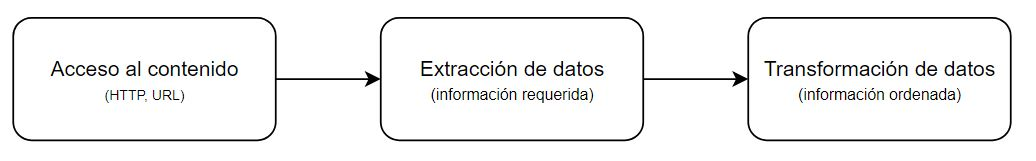
\includegraphics[width=6in]{web-scraping-phases.jpg}
\caption{Fases del web scraping}
\label{img:web-scraping-phases}
\end{figure}

Por otro lado, a lo largo del apéndice \ref{cha:funcionamiento basico de un web scraper}, se ilustra el
funcionamiento del agente software en cada una de las fases descritas anteriormente, así como de su
comportamiento con el servidor web al que se desea acceder.

\subsection{Herramientas software disponibles}
\label{subsec:herramientas software disponibles}

El software disponible que emplean los \emph{web scrapers} puede dividirse en varios enfoques, ya sean 
bibliotecas de programación de propósito general, \emph{frameworks}, o entornos de escritorio.

Por lo general, tanto los \emph{frameworks} como los entornos de escritorio presentan una solución más
sencilla e integradora con respecto a bibliotecas de programación. Esto es debido a que ambos, no se ven
afectados a los posibles cambios HTML de los recursos a los que accede. Además, estas necesitan la
integración de otras múltiples bibliotecas adicionales para el acceso, análisis y extracción del contenido.

Este trabajo se desarrolla sobre bibliotecas de programación, las cuales se implementan como un programa
software convencional utilizando estructuras de control y datos del propio lenguaje. Por lo general,
bibliotecas como \emph{curl \cite{curl-cran}} conceden acceso al sitio web deseado haciendo uso del
protocolo HTTP, mientras que los contenidos extraídos se analizan a través de funciones como la
coincidencia de expresiones regulares y la tokenización.

Comprender como las bibliotecas obtienen los datos de los sitios web, pasa por conocer las diferentes
formas en las que los documentos HTML se organizan. Existen dos técnicas, dependiendo si se realiza un
renderizado previo o no \cite{tfg-daniel-francisco-lopez}. La primera técnica consiste simplemente en
parsear, es decir, realizar un análisis léxico-sintáctico sobre estructuras XML o HTML. Se suelen emplear
expresiones \emph{XPath} o selectores CSS para su realización. Por otro lado, si es necesario que parte de 
la lógica del sitio web pase al lado del cliente, este deberá pasar por un proceso de renderizado previo.

Con el paso del tiempo, cada vez se extiende más el uso de bibliotecas de desarrollo como \textbf{JQuery}, 
encargadas de pasar parte de la lógica del lado del servidor al lado del cliente con el objetivo de favorecer 
la interactividad. Estas páginas no podrán ser analizadas si no se renderizan antes.

\subsubsection{XPath}
\label{subsubsec:xpath}

\emph{XPath} es un lenguaje que permite construir expresiones que recorren y procesan un documento XML
\cite{css-xpath-lilland}. Puede utilizarse para navegar por documentos HTML, ya que este es un lenguaje
similar en cuanto a estructura a XML. Es comúnmente usado en el \emph{web scraping} para extraer datos
de documentos HTML, además utiliza la misma notación empleada en las URL para navegar por la estructura
del sitio web en cuestión.

\subsubsection{Selectores CSS}
\label{subsubsec:selectores CSS}

El segundo método de extracción de datos en documento HTML se realiza a través de lo que se conoce como
selectores CSS \cite{css-xpath-lilland}. CSS es el lenguaje utilizado para dar estilo a los documentos
HTML, por otro lado, los selectores son patrones que se utilizan para hacer coincidir y extraer elementos
HTML basados en sus propiedades CSS.

Hay múltiples sintaxis de selector diferentes, estas se corresponden con la forma en la que el documento
CSS está estructurado. En el fragmento de código \ref{cod:extraccion de datos de interes del documento}
se hace uso de los selectores \emph{'.text-primary'} y \emph{'.lister-item-header a'} para acceder al
contenido web deseado.

\subsection{Tipologías}
\label{subsec:tipologias}

Dependiendo de como se acceda y extraiga la información, existen dos técnicas de \emph{web scraping}. Se 
mencionan los siguientes supuestos a continuación:

\begin{itemize}
\item Si la información que se almacena no procede de sitios web concretos, sino que durante el análisis
de páginas web se encuentran enlaces que retroalimentan el análisis de otras nuevas, el método se conoce
como \emph{web crawling} \cite{Andreas-Mehlfuhrer}.

\item Por el contrario, si la información se extrae de sitios web concretos, donde ya se conoce como extraer 
y generar un valor por la misma, la técnica se conoce como \emph{web scraping} genérico. Mientras que en 
el \emph{web crawling} el resultado de ejecución es la obtención de nuevas páginas, en el \emph{web scraping} 
el resultado es la propia información.
\end{itemize}

Es decir, la principal diferencia entre ambas, es que mientras los \emph{web scrapers} extraen información 
de páginas webs concretas, los \emph{web crawlers} almacenan y acceden a las páginas a través de los enlaces
contenidos en las mismas. En la figura \ref{img:web-scraping-phases} se mostraba la arquitectura en fases
de un \emph{web scraper}, veamos a continuación como es la arquitectura de un \emph{web crawler}.

\begin{figure}[tphb]
\centering
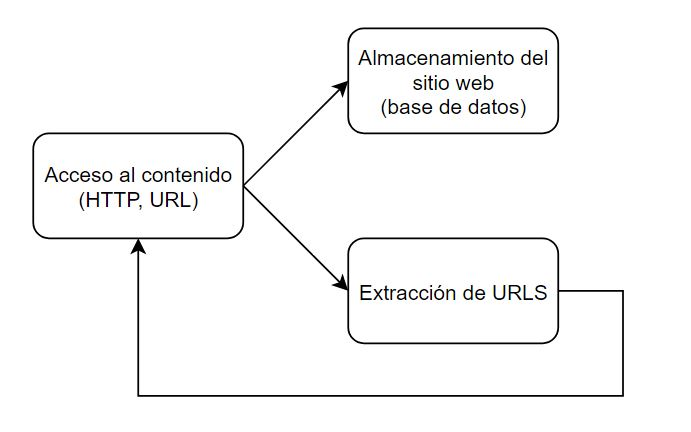
\includegraphics[width=4.3in]{web-crawler-phases.jpg}
\caption{Fases del web crawling}
\label{img:web-crawler-phases}
\end{figure}

Ya sea empleando cualquiera de estas dos tipologías, existen páginas que no pueden ser analizadas o
rastreadas. Esto es debido a que algunos sitios web solo están disponibles con una autorización previa, o
necesitan información especial para su acceso.

\section{Posibilidades prácticas del web scraping}
\label{sec:posibilidades practicas del web scraping}

Son muchas las aplicaciones prácticas de la minería web, la mayoría de estas entran en el ámbito de la
ciencia de los datos. En la siguiente lista se exponen algunos casos de su uso en la vida real
\cite{web-scraping-seppe}:

\begin{itemize}
    \item Bancos y otras instituciones financieras utilizan minería web para analizar a la competencia.
    Inversores también utilizan \emph{web scraping}, para hacer un seguimiento de artículos de prensa 
    relacionados con los activos de su cartera.

    \item En las redes sociales se emplea minería de datos para conocer la opinión de la gente a cerca de 
    un determinado tema.

    \item Existen aplicaciones capaces de analizar diferentes sitios web y encontrar los mismos productos 
    a precio reducido. Incluso capaces de detectar ofertas de artículos a tiempo récord.

    \item etcétera
\end{itemize}

El minado web contiene infinidad de aplicaciones, muy diversas e interesantes, capaces de automatizar el
trabajo y conseguir la información de forma ordenada. No obstante, muchos sitios web ofrecen alternativas
como el uso de APIs o ficheros estructuras para el acceso a dichos datos.

En general, el \emph{web scraping} es una técnica que consume bastantes recursos, por lo que el desarrollador
debe limitar su uso si existen otras alternativas, como las APIs, que proporcionan los mismos resultados.

\section{Retos del web scraping}
\label{sec:retos del web scraping}

La forma en la que se crean los sistemas de extracción web se ha discutido desde diferentes perspectivas
a lo largo del tiempo. En la mayoría de casos se emplean métodos científicos como el aprendizaje automático,
la lógica o el procesamiento del lenguaje natural para lograr su implementación.

Uno de los principales retos a afrontar tiene relación con las fuentes cambiantes de información. A menudo,
una herramienta de extracción tiene que obtener datos de forma rutinaria de una determinada página o sitio
web que puede evolucionar con el tiempo. Estos cambios se producen sin previo aviso, por lo que es bastante 
probable que los raspadores web se vean sometidos a cambios. Por ello, surge la necesidad crear herramientas 
flexibles capaces de detectar y afrontar modificaciones estructurales de las fuentes web relacionadas.

Otros problemas recaen sobre la información extraída. En primer lugar, uno de los aspectos que se deben
tener en cuenta al obtener información trata sobre la fiabilidad de la misma. Aunque la información exista
y sea analizada, puede que no sea correcta. La gramática y la ortografía en ocasiones suponen un problema
en la fase de análisis, ya que la información puede perderse o ser falsamente recogida. Por otro lado,
tanto aplicaciones que tratan con datos personales, como software de minado, deben ofrecer garantías de
privacidad. Además, los posibles intentos de violar la privacidad del usuario deben ser identificados
y contrarrestados a tiempo y de forma adecuada.

Puesto que multitud de técnicas de minería web requieren ayuda humana, un primer reto consiste en
proporcionar un alto grado de automatización, reduciendo así al máximo el esfuerzo humano. Sin embargo,
la ayuda humana puede desempeñar un papel importante a la hora de elevar el nivel de precisión alcanzado
por un sistema de extracción de datos web, por ello la clave está en encontrar el equilibrio perfecto entre
automatización e intervención humana.

Por último, a pesar de que las herramientas de \emph{web scraping} han evolucionado con el tiempo, los 
aspectos legales están algo inexplorados pues dependen de los términos y condiciones de cada sitio web en 
cuestión.

\section{Aspectos ético-legales del web scraping}
\label{sec:aspectos etico-legales del web scraping}

Para comprender los aspectos legales del \emph{web scraping}, debemos recordar el robot o agente software
definido en el apartado \ref{subsec:extraccion de los datos}. Este agente software, previamente examinado
por el servidor, es el que se encarga de acceder y realizar un recorrido por el contenido web.

Durante el acceso al contenido, se espera que este agente se ajuste a los términos de uso del sitio en
cuestión, así como el cumplimiento del archivo \emph{'robots.txt'} \footnote{Archivo alojado en el
servidor web, que gestiona el tráfico del mismo e indica los documentos a los que no se debe acceder de
forma automática \cite{robots-txt}.}, con el objetivo de evitar accesos no deseados y sobrecargas en el
servidor.

Puesto que el documento \emph{'robots.txt'} no es de obligado cumplimiento, a lo largo de los años la
reputación del \emph{web scraping} ha decrecido de manera significativa. Muchos agentes software no siguen
las indicaciones determinadas, por lo que definir la cantidad de accesos y archivos a los que se accede
dependerá de la ética de cada desarrollador.

Con el objetivo de tener una cierta garantía de que nuestro agente software cumple con los aspectos
ético-legales, se deben tener en consideración las siguientes cuestiones \cite{legalidad-web-scraping}:

\begin{itemize}
    \item Leer los términos de uso de la página web en al que se vaya a realizar el minado.

    \item Inspeccionar y cumplir con el documento \emph{'robots.txt'}, para ser capaces de identificar los 
    accesos del servidor.

    \item Realizar peticiones al servidor de forma controlada. Puede que el índice de solicitudes al 
    servidor no este especificado en el documento, si esto sucede debemos determinar un número de solicitudes 
    razonable, por ejemplo, una solicitud por segundo.
\end{itemize}



















\chapter{Bibliotecas de programación orientadas al web scraping}
\label{cha:bibliotecas de programacion orientadas al web scraping}

\section{Búsqueda de bibliotecas destinadas al web scraping}
\label{sec:busqueda de bibliotecas destinadas al web scraping}

Como se especificó en la sección \ref{sec:objetivo y limitaciones} este trabajo se limitará a realizar
una comparativa de los programas software de minado web más frecuentes. Esta comparativa se efectúa con el
fin de conocer cuál o cuáles de estos programas o paquetes software son los más rentables para este propósito.

¿Como saber que paquetes software destinados al minado web son los más comunes? Durante todo este capítulo
se procederá a la búsqueda, selección e introducción de programas software empleados para el \emph{web 
scraping}. Cabe destacar que Python y R serán los lenguajes de programación con los que se trabajará tanto 
para el desarrollo de la herramienta de comparación, como para el proceso de extracción de datos.

El primer paso consiste en buscar todos los elementos posibles que conforman la población de paquetes
software del mercado, ya sean de Python o R. La búsqueda de estos paquetes se ha realizado a través de las 
distintas fuentes de información mostradas a continuación:

\begin{enumerate}
  \item GitHub \cite{github}. Gran parte de los desarrolladores de estos programas, publican su trabajo en
  estos repositorios de código abierto.
  \item CRAN \cite{cran}. The Comprehensive R Archive Network es una red de servidores ftp y web que
  almacena versiones idénticas de código y documentación para R.
  \item PyPi \cite{pypi}. Python Package Index es un repositorio de software para Python, útil para la
  búsqueda de paquetes de un determinado propósito.
\end{enumerate}

\section{Bibliotecas de Python encontradas durante el proceso de búsqueda}
\label{sec:bibliotecas de python encontradas durante el proceso de busqueda}

A continuación, se hará una breve sinopsis de las bibliotecas de Python encontradas. Esta sinopsis tiene 
como objetivo conocer el funcionamiento, funciones principales y proceso de extracción de las mismas.

Es posible que algunos de los paquetes hayan sido desarrollados tanto en R como en Python. En ese caso, por 
un lado, la introducción se realzará de forma conjunta, sin embargo, será interesante ver el código del 
mismo en ambos casos y como se comportan estos ante los distintos test de evaluación.

Antes de comenzar con la sinopsis de bibliotecas, es conveniente revisar el apéndice \ref{cha:analizadores 
empleados en los paquetes de web scraping}, donde se realiza una breve introducción de aquellos analizadores 
empleados en las mismas. Los 'emparejamientos' entre biblioteca-analizador se recogen en la tabla 
\ref{tab:emparejamientos biblioteca-analizador} a modo de resumen.

\begin{table}[h]
  \begin{center}
  \begin{tabular}{| c | c | c | c | c | c | c |} \hline 
    \textbf{inscriptis} & \textbf{dragnet} & \textbf{boilerpy} & \textbf{libextract} & \textbf{news-please} & \textbf{justext} & \textbf{goose3} \\ \hline
    lxml & lxml & html parser & lxml & lxml & lxml & lxml \& html parser \\ \hline
  \end{tabular}

  \hfill \break

  \begin{tabular}{| c | c | c | c | c | c |} \hline 
    \textbf{html2text} & \textbf{readability} & \textbf{trafilatura} & \textbf{beautiful soup} & \textbf{newspaper3k} & \textbf{html\_text}  \\ \hline
    html parser & lxml & lxml & lxml \& html5lib \& html & lxml & lxml \\ \hline
  \end{tabular}

  \caption{Emparejamientos biblioteca-analizador}
  \label{tab:emparejamientos biblioteca-analizador}
  \end{center}
\end{table}

Ya sea porque determinadas bibliotecas permiten al desarrollador seleccionar entre varios tipos de 
analizadores, o bien porque múltiples de ellos son necesarios para el correcto funcionamiento de la 
extracción, muchas de estas bibliotecas hacen uso de más de un analizador en su código.

\subsection{inscriptis}
\label{subsec:inscriptis}

Además de ser una biblioteca de conversión de HTML a texto basada en Python, \textbf{inscriptis}
\cite{inscriptis} también tiene soporte como línea de comandos o como servicio web para tablas anidadas.
A pesar de sus múltiples funcionalidades, esta sección se centra en \textbf{inscriptis} como biblioteca de
programación.

\subsubsection{Estructura de la solución}
\label{subsubsec:estructura de la solucion}

A diferencia de otros algoritmos de extracción, \textbf{inscriptis} no solo tiene en cuenta la calidad del 
texto extraído, la estructura del mismo también es muy importante. Esto provoca que el resultado obtenido 
se acerque más a un posible resultado aplicando el método tradicional a través de cualquier navegador web.

Se muestra a continuación una pequeña comparación entre la extracción de texto de \textbf{Beautiful Soup}
\ref{subsec:beautiful soup}, con la extracción de texto de \textbf{inscriptis}, donde se tiene un fragmento 
HTML como el siguiente como objeto de prueba.

\begin{Schunk}
  \begin{Soutput}
      <li>first</li>
      <li>second</li>
  \end{Soutput}
\end{Schunk}

Se emplea en primer lugar el método \emph{get\_text()} propio de \textbf{Beautiful Soup} sobre el fragmento 
HTML anterior.

\begin{Schunk}
  \begin{Soutput}
    # firstsecond
  \end{Soutput}
\end{Schunk}

Se puede observar que el formato obtenido no es el adecuado, puesto que no se ha respetado la estructura
del documento base. Sin embargo, si se aplica \textbf{inscriptis} sobre el mismo fragmento HTML, la salida 
obtenida sería la siguiente:

\begin{Schunk}
  \begin{Soutput}
    # first
    # second
  \end{Soutput}
\end{Schunk}

El algoritmo no solo admite construcciones tan simples como la anterior, también es posible analizar
construcciones mucho más complejas, como las tablas anidadas, y subconjuntos de atributos HTML o CSS, donde
es esencial una conversión precisa de HTML a texto.

\subsubsection{Reglas de anotación}
\label{subsubsec:reglas de anotacion}

La técnica que se emplea en este caso se conoce como reglas de anotación, es decir, mapeos que permiten 
realizar anotaciones sobre el texto extraído. Estas anotaciones se basan en la información estructural y 
semántica codificada en las etiquetas y atributos HTML utilizados para controlar la estructura y diseño 
del documento original. Con el fin de asignar etiquetas y/o atributos HTML a las anotaciones, se utiliza 
lo que se conoce como perfil de anotaciones, algo parecido a un diccionario. 


\begin{table}[h]
  \begin{center}
  \begin{tabular}{| c | c |} \hline 
    h1 & ['heading', 'h1'] \\ \hline
    h2 & ['heading', 'h2'] \\ \hline
    b & ['emphasis'] \\ \hline
    div\#class=toc & ['table-of-contents'] \\ \hline
    \#class=FactBox & ['fact-box'] \\ \hline
    \#cite & ['citation'] \\ \hline
  \end{tabular}
  \caption{inscriptis - Perfil de anotaciones}
  \label{tab:inscriptis - perfil de anotaciones}
  \end{center}
\end{table}

Si observamos el diccionario mostrado en la tabla \ref{tab:inscriptis - perfil de anotaciones}, las 
etiquetas de tipo cabecera producen anotaciones de tipo \emph{hn}, una etiqueta \emph{<div>} con una 
clase que contiene el valor \emph{toc} da como resultado la anotación \emph{table-of-contents}, y todas 
las etiquetas con un atributo \emph{cite} se anotan como \emph{citation}.

A modo de ejemplo, y con el fin de mostrar el correcto etiquetado del algoritmo, imaginemos que se dispone 
el fragmento de un documento HTML como el mostrado a continuación y unas reglas de anotación como las 
mostradas en la tabla \ref{tab:inscriptis - perfil de anotaciones}.

\begin{Schunk}
  \begin{Soutput}
    <h1>Chur</h1>
    <b>Chur</b> is the capital and largest town of the Swiss 
    canton of the Grisons and lies in the Grisonian Rhine Valley.
  \end{Soutput}
\end{Schunk}

A partir de este ejemplo, y basándonos en el diccionario anterior, la salida esperada debería ser una 
etiqueta de cabecera y otra de énfasis, veamos el resultado que proporciona el proceso de asignación.

\begin{Schunk}
  \begin{Soutput}
    {
      "text": "Chur\n\nChur is the capital and largest town of the Swiss 
              canton of the Grisons and lies in the Grisonian Rhine Valley.",
      "label": [[0, 4, "heading"], [0, 4, "h1"], [6, 10, "emphasis"]]
    }
  \end{Soutput}
\end{Schunk}

Como era de esperar la obtención del texto es precisa, pero no solo del texto sino de su estructura. Además,
la asignación de etiquetas también se ha realizado de forma correcta. Se muestra en el fragmento de código
\ref{cod:inscriptis - uso de reglas de anotacion} como se pueden emplear las reglas de anotación dentro de 
un programa.

\begin{codefloat}
  \inputencoding{latin1}
  \lstinputlisting[style=CppExample]{scripts/inscriptis-reglas-anotacion.py}
  \inputencoding{utf8}
  \caption{inscriptis - Uso de reglas de anotación}
  \label{cod:inscriptis - uso de reglas de anotacion}
\end{codefloat}

\subsubsection{Postprocesamiento}
\label{subsubsec:postprocesamiento}

Además, \textbf{inscriptis} da la posibilidad al usuario de realizar una fase de postprocesamiento donde 
las anotaciones se realizan en un formato determinado. Un primer tipo de postprocesamiento es el que se 
conoce como \emph{surface}, donde se retorna una lista de mapeos entre la superficie de anotación y su 
etiqueta.

\begin{Schunk}
  \begin{Soutput}
    [['heading', 'Chur'],
      ['emphasis': 'Chur']]
  \end{Soutput}
\end{Schunk}

En segundo lugar, el postprocesamiento tipo xml retorna una etiqueta de versión adicional, propia de un
documento XML convencional.

\begin{Schunk}
  \begin{Soutput}
    <?xml version="1.0" encoding="UTF-8" ?>
    <heading>Chur</heading>

    <emphasis>Chur</emphasis> is the capital and largest town of the 
    Swiss canton of the Grisons and lies in the Grisonian Rhine Valley.
  \end{Soutput}
\end{Schunk}

Por último, el postprocesamiento en tipo html crea un documento HTML que contiene el texto convertido y 
resalta todas las anotaciones. Se muestra en la figura \ref{img: inscriptis - postprocesamiento html} un 
ejemplo de la salida obtenida.

\begin{figure}[tphb]
  \centering
  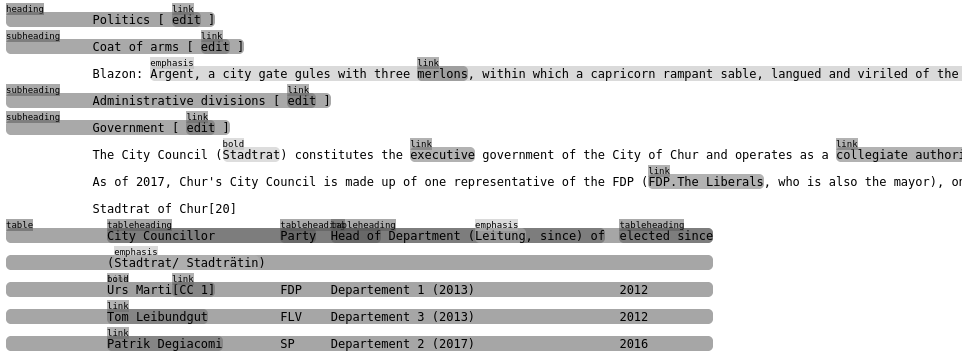
\includegraphics[width=6.3in]{inscriptis-html-postprocessor.png}
  \caption{inscriptis - Postprocesamiento html}
  \label{img: inscriptis - postprocesamiento html}
\end{figure}

\subsection{Beautiful Soup}
\label{subsec:beautiful soup}

Una de las bibliotecas de Python más comunes en el ámbito del \emph{web scraping} es \textbf{Beautiful Soup}
\cite{beautifulsoup}, la cual está diseñada para extraer datos de documentos XML y HTML. Como se muestra
en la tabla \ref{tab:emparejamientos biblioteca-analizador} y a diferencia del resto de bibliotecas,
\textbf{Beautiful Soup} permite determinar el tipo de analizador que se empleará en la extracción, lo que
flexibiliza el proceso de navegación, búsqueda y modificación de documentos.

\subsubsection{Multiplicidad de analizadores}
\label{subsubsec:multiplicidad de analizadores}

\textbf{Beautiful Soup} tiene a \emph{html.parse} como analizador estándar de documentos HTML, pero admite 
varios analizadores de terceros. En la tabla \ref{tab:beautiful soup - analizadores disponibles} se muestran 
los distintos analizadores disponibles, así como un pequeño resumen de las ventajas y desventajas de estos.

\begin{table}[h]
  \begin{center}
  \begin{tabular}{| c | c | c | c |}
  \hline \textbf{Tipo de analizador} & \textbf{Forma de uso} & \textbf{Ventajas} & \textbf{Desventajas} \\ \hline
  html & bs(markup, "html.parser") & Notablemente rápido & Mas lento que lxml \\
  lxml html & bs(markup, "lxml") & Muy rapido & Dependencia de C \\
  lxml xml & bs(markup, "xml") & Muy rápido y soporta xml & Dependencia de C \\
  html5lib & bs(markup, "html5lib") & Analiza igual que un buscador & Muy lento \\ \hline
  \end{tabular}
  \caption{Beautiful Soup - Analizadores disponibles}
  \label{tab:beautiful soup - analizadores disponibles}
  \end{center}
\end{table}

El empleo de distintos analizadores supondrá una importancia menor si se aplica sobre documentos bien
formados, pues la solución aportada presentará la misma estructura que el propio documento original. En
caso contrario, el uso de múltiples analizadores creará diferentes soluciones para un mismo documento.

Se emplea el analizador \emph{lxml} sobre un documento HTML sencillo pero con erratas. Vemos como la solución 
aportada propone la inclusión de nuevas etiquetas \emph{<html>} y \emph{<body>}, sin embargo, ¿qué ha 
ocurrido con la etiqueta \emph{</p>}?.

\begin{Schunk}
  \begin{Soutput}
    >>> BeautifulSoup("<a></p>", "lxml")
    # <html><body><a></a></body></html>
  \end{Soutput}
\end{Schunk}

En lugar de ignorar la etiqueta \emph{</p>} como lo hace \emph{lxml}, el analizador html5lib la empareja 
con una etiqueta \emph{<p>} de apertura. También añade una etiqueta \emph{<head>} que el analizador 
\emph{lxml} había obviado.

\begin{Schunk}
  \begin{Soutput}
    >>> BeautifulSoup("<a></p>", "html5lib")
    # <html><head></head><body><a><p></p></a></body></html>
  \end{Soutput}
\end{Schunk}

Al igual que \emph{lxml}, \emph{html.parse} ignora la etiqueta de cierre \emph{</p>}. Podemos observar que 
este analizador ni siquiera intenta crear un documento HTML bien formado añadiendo etiquetas \emph{<html>} 
o \emph{<body>}.

\begin{Schunk}
  \begin{Soutput}
    >>> BeautifulSoup("<a></p>", "html.parser")
    # <a></a>
  \end{Soutput}
\end{Schunk}

Como vemos diferentes analizadores crearan diferentes soluciones en caso de que el documento a analizar no 
este bien formado. Por ello, si se desea analizar múltiples documentos de los que no conocemos su origen o 
estructura, sería conveniente especificar el tipo de analizador con el fin del obtener la solución deseada.

\subsubsection{Sopa de objetos}
\label{subsubsec:sopa de objetos}

El proceso de extracción que se emplea en este algoritmo es sencillo. En primer lugar, el documento ya sea 
HTML o XML se convierte por completo en caracteres unicode. Tras ello se crea un árbol de objetos donde 
cada uno de ellos representa una etiqueta o \emph{tag} del propio documento. Finalmente, un analizador 
especificado por parámetro, recorre el árbol buscando las partes del mismo que se desean.

\begin{figure}[tphb]
  \centering
  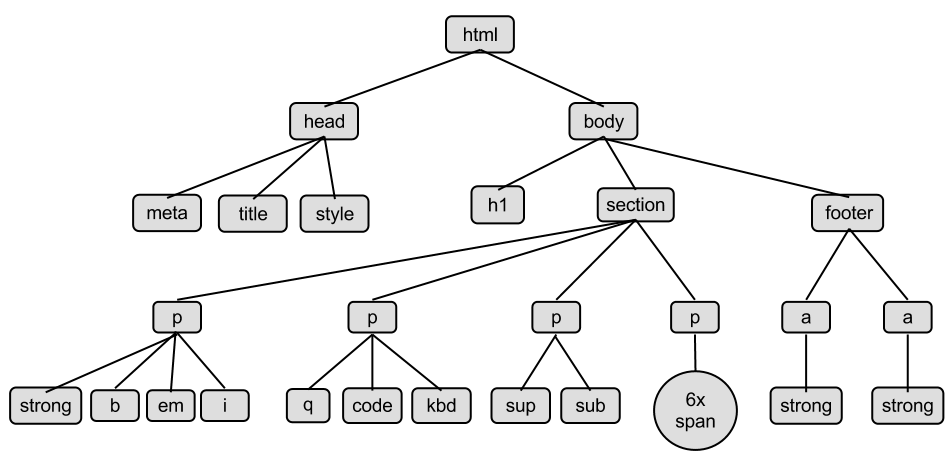
\includegraphics[width=4.5in]{bs-parse-tree.png}
  \caption{Arbol de objetos}
  \label{img:arbol de objetos}
\end{figure}

Este algoritmo, no solo permite el recorrido automático del árbol en busca del texto del documento al
completo, sino que permite además la posibilidad de recorrer el mismo de forma manual, por lo que es posible
acceder a todos los objetos del árbol empleando métodos de navegación como \emph{soup.head, soup.parent,
soup.next\_sibling, ...}.

\subsection{jusText}
\label{subsec:justext}

\textbf{jusText} \cite{justext} es una herramienta para eliminar el contenido repetitivo, como los enlaces
de navegación, encabezados y pies de página de los documentos HTML. Este algoritmo, está diseñado para
preservar el texto que contiene frases completas.

\subsubsection{Preprocesamiento}
\label{subsubsec:preprocesamiento}

Previamente a cualquier fase y con el fin de facilitar el trabajo heurístico, se realiza un preprocesamiento 
del documento HTML. Durante este proceso, se elimina el contenido de ciertas etiquetas como \emph{<header>}, 
\emph{<style>} y \emph{<script>}. Además, el contenido de etiquetas como \emph{<select>} se clasifica 
inmediatamente como contenido basura. Lo mismo ocurre con los bloques que contienen ciertos símbolos 
especiales como el de copyright ©.

\subsubsection{Segmentación}
\label{subsubsec:segmentacion}

Tras una previa fase de preprocesamiento, se procede a lo que se conoce como segmentación. La idea es formar 
bloques de texto dividiendo la página HTML por etiquetas. Una secuencia de dos o más etiquetas como 
\emph{<br>}, \emph{<div>, ...}, separaría los bloques. 

Para la segmentación de bloques, la clave es que los bloques largos y algunos bloques cortos pueden
clasificarse con una confianza muy alta. El resto de bloques cortos pueden clasificarse observando los
bloques circundantes. 

Aunque no sea habitual, puede ocurrir que el contenido de estos bloques no sea homogéneo, es decir, que
dentro de un mismo bloque haya una mezcla de información importante con contenido basura, denominado
\emph{boilerplate}. Se resumen a continuación algunos aspectos en relación.

\begin{itemize}
  \item Los bloques cortos que contienen un enlace son casi siempre del tipo \emph{boilerplate}.
  \item Los bloques que contienen muchos enlaces son casi siempre del tipo \emph{boilerplate}.
  \item Tanto los bloques buenos como los bloques de tipo \emph{boilerplate} tienden a crear grupos, es 
  decir, un bloque \emph{boilerplate} suele estar rodeado de otros bloques de su mismo tipo y viceversa.
  \item Los bloques largos que contienen texto gramatical forman parte del contenido valioso, mientras que 
  todos los demás bloques largos son casi siempre del tipo \emph{boilerplate}.
\end{itemize}

Con respecto al ultimo punto, decidir si un texto es gramatical o no puede ser complicado, \textbf{jusText} 
emplea una simple heurística basada en el volumen de palabras con sentido gramatical. Mientras que un texto 
gramatical suele contener un cierto porcentaje de estas palabras, los contenidos de tipo \emph{boilerplate} 
suelen carecer de ellas.

\subsubsection{Clasificación de bloques}
\label{subsubsec:clasificacion de bloques}

Tras la fase de preprocesamiento y segmentación se procede a la clasificación de bloques, donde a cada uno
de estos bloques se le asigna una clase dependiendo de su naturaleza. En el fragmento de código 
\ref{cod:justext - algoritmo de clasificacion} se muestra paso a paso como se determina el tipo de clase 
para cada bloque.

\begin{codefloat}
  \inputencoding{latin1}
  \lstinputlisting[style=CppExample]{scripts/justext-clasificacion.py}
  \inputencoding{utf8}
  \caption{jusText - Algoritmo de clasificación}
  \label{cod:justext - algoritmo de clasificacion}
\end{codefloat}

Analizando el algoritmo, se observa que se definen dos tipos de variables, la densidad y la longitud. 
Mientras que la longitud es el número de caracteres por bloque, la densidad se define como la proporción 
de caracteres o palabras dentro de una etiqueta de tipo \emph{<a>}, o una lista de parada.

Además de los valores de densidad y longitud, el algoritmo toma como parámetros dos enteros definidos como
\emph{LENGTH\_LOW} y \emph{LENGTH\_HIGH}, y también tres números de coma flotante, \emph{MAX\_LINK\_DENSITY},
\emph{STOPWORDS\_LOW} y \emph{STOPWORDS\_HIGH}. Los dos primeros establecen los umbrales para dividir los 
bloques por su longitud. Los dos últimos dividen los bloques por la densidad de palabras de parada en bajos, 
medianos y altos.

Si volvemos a observar el algoritmo \ref{cod:justext - algoritmo de clasificacion}, nos damos cuenta de
que solo se ha realizado una clasificación real sobre los bloques de tamaño medio y largo. En la tabla
\ref{tab:justext - clasificacion de bloques long & medium size} se muestra a modo de resumen como se actúa 
sobre este tipo de bloques.

\begin{table}[h]
  \begin{center}
  \begin{tabular}{| c | c | c |}
  \hline \textbf{Block size} & \textbf{Stopwords density} & \textbf{Class} \\ \hline
  medium size & low & bad \\ \hline
  long & low & bad \\ \hline
  medium size & medium & near-good \\ \hline
  long & medium & near-good \\ \hline
  medium size & high & near-good \\ \hline
  long & high & good \\ \hline
  \end{tabular}
  \caption{jusText - Clasificación de bloques long \& medium size}
  \label{tab:justext - clasificacion de bloques long & medium size}
  \end{center}
\end{table}

\subsubsection{Reclasificación de bloques}
\label{subsubsec:reclasificacion de bloques}

¿Qué ocurre entonces con los bloques cortos y los bloques casi buenos? La reclasificación en este caso se 
realiza en función de los bloques circundantes. Los bloques ya clasificados como buenos o malos sirven 
como piedras base en esta etapa y su clasificación se considera fiable, por lo que nunca se modifica. Esta 
reclasificación se puede ver resumida en la figura \ref{img:justext - reclasificacion de bloques}.

\begin{figure}[tphb]
  \centering
  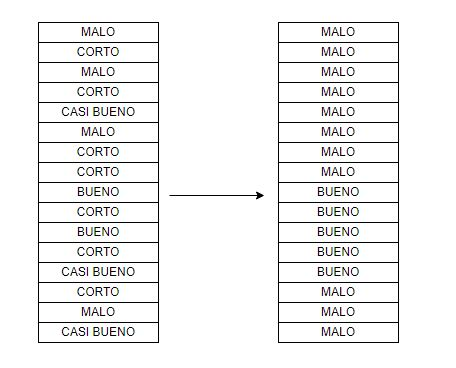
\includegraphics[width=3.6in]{justext-blocks-classification.jpg}
  \caption{jusText - Reclasificación de bloques}
  \label{img:justext - reclasificacion de bloques}
\end{figure}

La idea que subyace a la reclasificación es que los bloques \emph{boilerplate} suelen estar rodeados de 
otros bloques \emph{boilerplate} y viceversa. Los bloques casi buenos suelen contener datos útiles del 
corpus si se encuentran cerca de bloques buenos. Los bloques cortos suelen ser útiles sólo si están rodeados 
de bloques buenos por ambos lados.

\subsubsection{Bloques de cabecera}
\label{subsubsec:bloques de cabecera}

En cuanto a los bloques de cabecera, aquellos encerrados en etiquetas del tipo \emph{<h1>}, \emph{<h2>}, 
..., son tratados de una manera especial. El objetivo es conservar estos bloques en los textos determinados 
como buenos.

Para el tratamiento especial de bloques de cabecera se añaden dos etapas. La primera etapa, conocida como 
preprocesamiento, se ejecuta justamente después de la clasificación y justo antes de la reclasificación de 
bloques. La segunda etapa, conocida como postprocesamiento, se ejecuta después de la reclasificación.

\begin{enumerate}
  \item Clasificación de bloques.
  \item \textbf{Preprocesamiento de bloques de cabecera}.
  \item Reclasificación de bloques.
  \item \textbf{Postprocesamiento de bloques de cabecera}.
\end{enumerate}

Durante esta fase de preprocesamiento, se buscan bloques de cabecera cortos que precedan a bloques buenos, 
y que al mismo tiempo no haya más caracteres entre el bloque de cabecera y el bloque bueno. El propósito 
de esto es preservar los bloques cortos entre el encabezado y el texto bueno que, de otro modo, podrían 
ser seleccionados como malos durante el proceso de reclasificación.

Por otro lado, en el postprocesamiento, se buscan de nuevo bloques de cabecera que precedan a bloques
buenos, y que al mismo tiempo no haya más caracteres entre el bloque de cabecera y el bloque bueno. El
propósito es que algunas cabeceras cortas y casi buenas puedan clasificarse como buenas si preceden a
bloques buenos que, de otro modo, habrían sido clasificadas como malas tras de la reclasificación.

\subsection{news-please}
\label{subsec:news-please}

Otro \emph{web scraper}, y al mismo tiempo \emph{web crawler}, de código abierto es \textbf{news-please}
\cite{news-please}. Esta biblioteca está desarrollada para cumplir cinco requisitos: extracción de
noticias de cualquier sitio web, extracción completa del sitio web, alta calidad de la información
extraída, facilidad de uso y mantenibilidad.

A diferencia de otras bibliotecas ya mencionadas anteriormente, se emplean herramientas ya existentes las 
cuales se amplían con nuevas funcionalidades con el objetivo de cumplir con los requisitos señalados.

\begin{figure}[tphb]
  \centering
  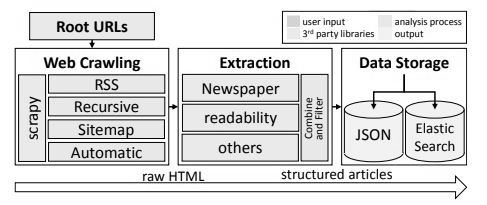
\includegraphics[width=4.5in]{newsplease-processing.jpg}
  \caption{news-please - Proceso de scraping y crawling}
  \label{img:news-please - proceso de scraping y crawling}
\end{figure}

\subsubsection{Web crawling en news-please}
\label{subsubsec:web crawling en news-please}

En cuanto al proceso de \emph{web crawling}, primero se descarga el documento y en segundo lugar, con el 
objetivo de encontrar todos los artículos publicados en dicho documento, se procede con el \emph{crawling}. 
Como se muestra en la figura \ref{img:news-please - proceso de scraping y crawling}, para este proceso se 
dispone de cuatro técnicas diferentes.

La primera técnica se conoce como RSS, en la que se analizan canales RSS con el objetivo de encontrar 
artículos recientes. Un RSS \cite{rss-sitemaps} es un tipo de formato de datos utilizado para proporcionar 
a los usuarios contenidos actualizados con frecuencia.

En segundo lugar, se emplea un seguimiento recursivo de los enlaces internos en las páginas rastreadas.
El uso del \emph{framework} \emph{scrapy} es fundamental independientemente de la técnica.

La tercera técnica consiste en analizar los \emph{sitemaps} en busca de enlaces a todos los artículos. Un 
\emph{sitemap} \cite{rss-sitemaps} es un archivo que enumera las URL's visibles de un determinado sitio, 
cuyo objetivo principal es revelar dónde pueden buscar contenido las máquinas.

Finalmente se prueba con el \emph{crawling} a través de los \emph{sitemaps} y en caso de que se produzca 
cualquier error se vuelve a la técnica de \emph{crawling} recursiva.

Estos cuatro enfoques también pueden combinarse, por ejemplo, iniciando dos instancias en paralelo, una en 
modo automático para obtener todos los artículos publicados hasta el momento y otra instancia en modo RSS 
para recuperar los artículos recientes.

\subsubsection{Web scraping en news-please}
\label{subsubsec:web scraping en news-please}

Para el proceso de \emph{web scraping}, se emplean herramientas ya existentes en el mercado con el objetivo 
de obtener la información deseada, título, contenido principal, autor, fecha... Herramientas como 
\textbf{Newspaper3k} \ref{subsec:newspaper3k} o \textbf{Readability} \ref{subsec:readability} son utilizadas 
para este proceso de extracción.

\begin{codefloat}
  \inputencoding{latin1}
  \lstinputlisting[style=CppExample, showstringspaces=false]{scripts/newsplease-scrape.py}
  \inputencoding{utf8}
  \caption{news-please - Extracción de contenido relevante}
  \label{cod:news-please - extraccion de contenido relevante}
\end{codefloat}

Una vez que el contenido relevante ha sido extraído, se almacena de forma estructurada en determinados
archivos de forma que este pueda ser consultado posteriormente.

\subsection{Libextract}
\label{subsec:libextract}

\textbf{Libextract} \cite{libextract} es una biblioteca de extracción de datos con capacidad estadística
que funciona con documentos HTML y XML, escrita en Python. En cuanto al algoritmo de extracción empleado,
\textbf{eatiht}, funciona en base a una simple suposición en la cual los datos aparecen como colecciones 
de elementos repetitivos.

\subsubsection{eatiht como algoritmo de partición}
\label{subsubsec:eatiht como algoritmo de particion}

\textbf{eatiht} \cite{eatiht} es una posible solución en una línea de muchas soluciones imperfectas a uno 
o más problemas en algún subcampo de la extracción de datos. En pocas palabras, este algoritmo intenta 
extraer el texto central de un sitio web determinado.

Se trabaja con dos supuestos, en primer lugar se determina que el texto considerado como valioso es largo, 
mientras que los textos 'basura' suelen disponer de una menor cantidad de información. Por otro lado, se 
determina que los textos de valor vienen agrupados.

Imaginemos un documento HTML sencillo en el que aplicando una determinada expresión \emph{XPath} como la 
siguiente, \emph{/text()[string-length(normalize-space()) > 20]}, se seleccionen todos los nodos de texto 
que tengan una longitud de cadena superior a veinte.

\begin{Schunk}
  \begin{Soutput}
    /html/body/div/article
    /html/body/div/div
    /html/body/div/footer
  \end{Soutput}
\end{Schunk}

Dada una posible solución como la anterior, se debe contar el numero de nodos hijo de cada uno con el 
objetivo de crear una distribución de frecuencias de cada conjunto a través de un histograma.

\begin{Schunk}
  \begin{Soutput}
    /html/body/div/article   | — — — —
    /html/body/div/div       | —
    /html/body/div/footer    | —
  \end{Soutput}
\end{Schunk}

Tras este proceso y con una simple comprensión de la lista de conjuntos, es posible adquirir algunos, pero 
no todos los nodos de texto que existen en el subárbol deseado. Veamos el funcionamiento de dicho algoritmo.

\begin{codefloat}
  \inputencoding{latin1}
  \lstinputlisting[style=CppExample, showstringspaces=false]{scripts/libextract-eatiht.py}
  \inputencoding{utf8}
  \caption{Libextract - Funcionamiento de eatiht}
  \label{cod:libextract - funcionamiento de eatiht}
\end{codefloat}

\subsection{html\_text}
\label{subsec:html_text}

\textbf{html\_text} \cite{html-text} es una biblioteca de Python encargada de convertir un documento HTML
en texto plano. Las principales diferencias frente a algoritmos como \textbf{Beautiful Soup},
\ref{subsec:beautiful soup} donde se emplean expresiones del tipo \emph{.get\_text()}, o frente a expresiones
\emph{XPath} como \emph{.xpath('//text()')}, son las siguientes:

\begin{enumerate}
  \item El texto extraído en este caso, no contiene código JavaScript del propio documento, así como 
  comentarios o cualquier contenido que no sea visible por el usuario.
  \item La normalización de espacios también se tiene en cuenta, pero de una manera más inteligente que
  con el uso simple de expresiones \emph{XPath}, \emph{.xpath('normalize-space())}, ya que añade espacios 
  alrededor de los elementos en línea, y evitar añadir espacios extra para la puntuación.
  \item Se añaden nuevas líneas de forma frecuente, por ejemplo después de los encabezados o párrafos, para 
  que el texto de salida se parezca más a cómo se presenta en los navegadores.
\end{enumerate}

En cuanto a la heurística, en primer lugar se limpia el documento empleando como instancia
\emph{lxml.html.clean.Cleaner}, y después, se procede con la conversión de árbol de objetos a texto,
empleando para ello lo que se conoce como \emph{'chunks'}.

\subsubsection{Normalización de espacio}
\label{subsubsec:normalizacion de espacio}

El uso habitual del algoritmo se consigue ejecutando la función de extracción de texto principal, de forma 
que un documento HTML se pasa por parámetro y se devuelve como salida la parte de información que se determina
como valiosa.

\begin{Schunk}
  \begin{Soutput}
    >>> html_text.extract_text('<h1>Hello</h1> world!')
    # 'Hello\n\nworld!'
  \end{Soutput}
\end{Schunk}

En cuanto a la estructura del texto extraído, es posible personalizar cómo se añaden nuevas líneas al mismo
utilizando los argumentos \emph{newline\_tags} y \emph{double\_newline\_tags}. De esta forma el algoritmo 
es capaz de distinguir de forma automática aquellas secciones del documento que deben ser separadas por 
línea simple o por doble línea.

\begin{Schunk}
  \begin{Soutput}
    NEWLINE_TAGS = frozenset([
      'article', 'aside', 'br', 'dd', 'details', 'div', 'dt', 'fieldset',
      'figcaption', 'footer', 'form', 'header', 'hr', 'legend', ...
    ])

    DOUBLE_NEWLINE_TAGS = frozenset([
      'blockquote', 'dl', 'figure', 'h1', 'h2', 'h3', 'h4', 'h5', 'h6', 'ol',
      'p', 'pre', 'title', 'ul'
    ])
  \end{Soutput}
\end{Schunk}

Imaginemos que se desea ejecutar \textbf{html\_text} sobre un documento HTML como el siguiente
\emph{<div>Hello</div> world!}, donde el texto principal esta separado por una etiqueta de tipo \emph{<div>}.
A partir de la gestión de espacio según el tipo de etiqueta, se determina la solución obtenida.

\begin{Schunk}
  \begin{Soutput}
    >>> newline_tags = html_text.NEWLINE_TAGS - {'div'}
    >>> html_text.extract_text('<div>Hello</div> world!',
    ...                        newline_tags=newline_tags)
    # 'Hello world!'
  \end{Soutput}
\end{Schunk}

\subsection{html2text}
\label{subsec:html2text}

\textbf{html2ext} \cite{html2text} es un script de Python que convierte un documento HTML a texto ASCII, 
el cual también resulta ser un formato de texto válido a HTML. Imaginemos que se dispone de un documento 
HTML sencillo como el siguiente, \emph{'<p><strong>Zed's</strong> dead baby, <em>Zed's</em> dead.</p>'}, 
veamos la salida obtenida:

\begin{Schunk}
  \begin{Soutput}
    >>> html2text("<p><strong>Zed's</strong> dead baby, <em>Zed's</em> dead.</p>"))
    # **Zed's** dead baby, _Zed's_ dead.
  \end{Soutput}
\end{Schunk}

Si por el contrario se desea que la solución sea limpia, es posible eliminar todos los caracteres de
marcado del texto obtenido empleando la función \emph{handle} como método de extracción.

\begin{Schunk}
  \begin{Soutput}
    >>> handle("<p><strong>Zed's</strong> dead baby, <em>Zed's</em> dead.</p>"))
    # Zed's dead baby, Zed's dead.
  \end{Soutput}
\end{Schunk}

En cuanto a la heurística de extracción, el algoritmo simplemente analiza el documento a través de
\emph{html.parser}, y a continuación envuelven todos los párrafos del texto proporcionado.

\subsection{Readability}
\label{subsec:readability}

Dado un documento HTML, \textbf{Readability} \cite{readability} extrae el cuerpo del texto principal del 
mismo. Previamente a la extracción de texto se produce una limpieza, donde se eliminan \emph{tags} y 
atributos del propio documento. Este preprocesamiento se lleva a cabo mediante el uso de expresiones 
regulares.

\subsubsection{Heurística de nodo candidato}
\label{subsubsec:heuristica de nodo candidato}

La heurística de esta biblioteca es similar a la empleada por \textbf{Goose3} \ref{subsec:goose3} para
calcular el mejor nodo del árbol. A partir de una puntuación dada para cada nodo se determina aquel cuya
puntuación se máxima con el objetivo de obtener el nodo con una mayor cantidad de información.

\begin{codefloat}
  \inputencoding{latin1}
  \lstinputlisting[style=CppExample, showstringspaces=false]{scripts/readability-menjor-candidato.py}
  \inputencoding{utf8}
  \caption{Readability - Selección del nodo candidato}
  \label{cod:readability - seleccion del nodo candidato}
\end{codefloat}

Una vez seleccionado dicho nodo, se busca en nodos hermanos con el objetivo de encontrar aquellos cuya
información esté relacionada con el mismo, y, por tanto, sean de valor.

\subsection{Trafilatura}
\label{subsec:trafilatura}

Al igual que muchas otras, \textbf{Trafilatura} \cite{trafilatura} es una herramienta de búsqueda de texto
en la web que descarga, analiza y extrae datos de documentos HTML. El algoritmo de extracción no solo se
centra en los metadatos, el cuerpo del texto o comentarios, también trata de conservar parte del formato
y la estructura de la página.

En cuanto a la heurística, esta se fundamenta en una cascada de filtros determinados por una serie de 
reglas y metodología del contenido. En las siguientes secciones se determinan los pasos que realiza el
algoritmo para una extracción exitosa.

\subsubsection{Delimitación de contenido}
\label{subsubsec:delimitacion de contenido}

El objetivo de esta primera fase es separar el contenido con valor del contenido basura o
\emph{boilerplate}. Para ello el algoritmo hace uso de expresiones \emph{XPath} dirigidas tanto a atributos 
HTML, como al contenido principal del documento.

\begin{Schunk}
  \begin{Soutput}
    DISCARD_XPATH = [
      '''.//*[(self::div or self::item or self::list or self::p or self...)][
      contains(@id, "related") or contains(@class, "nav") or 
      contains(@class, "subnav") or contains(@id, "cookie") or ...]'''
    ]
  \end{Soutput}
\end{Schunk}

Inicialmente, el uso de expresiones como las mostradas se emplea para excluir partes o secciones no deseadas 
del código HTML, por ejemplo la expresión \emph{<div class='nav'>} eliminaría todo el contenido que incluyese
cualquier etiqueta \emph{<div>} de tipo \emph{'navigation'}.

Tras esta exclusión de contenido \emph{boilerplate}, el algoritmo se centra nuevamente en el uso de 
expresiones \emph{XPath}, pero en este caso que abarquen todo el contenido de valor a extraer. Expresiones 
como \emph{<section id='entry-content'>} o como las mostradas a continuación, buscan partes de contenido
potencialmente valioso.

\begin{Schunk}
  \begin{Soutput}
    BODY_XPATH = [
      '''.//*[(self::article or self::div or self::main or self::section)][
      contains(@id, "content-main") or
      contains(@class, "entry-content") or 
      contains(@class, "content-main") or ...]'''
    ]
  \end{Soutput}
\end{Schunk}

Las mismas operaciones se realizan para los comentarios en caso de que estos formen parte de la extracción. 
Los nodos seleccionados del árbol HTML se procesan, es decir, se comprueba su relevancia y se simplifican 
en cuanto a su estructura HTML.

\begin{Schunk}
  \begin{Soutput}
    COMMENTS_XPATH = [
      '''.//*[(self::div or self::section or self::list)][
      contains(@id, 'commentlist') or 
      contains(@class, 'commentlist') or 
      contains(@class, 'comment-page') or ...]'''
    ]
  \end{Soutput}
\end{Schunk}

\subsubsection{Algoritmos de respaldo}
\label{subsubsec:algoritmos de respaldo}

Si se detecta que la extracción realizada ha sido defectuosa, se ejecuta lo que se conocen como algoritmos 
de respaldo. Estos algoritmos aplican una heurística basada en la longitud de las líneas, la relación 
texto/marcado y la posición/profundidad de los elementos en el árbol HTML.

\begin{codefloat}
  \inputencoding{latin1}
  \lstinputlisting[style=CppExample, showstringspaces=false]{scripts/trafilatura-respaldo1.py}
  \inputencoding{utf8}
  \caption{Trafilatura - Readability como algoritmo de respaldo}
  \label{cod:trafilatura - readability como algoritmo de respaldo}
\end{codefloat}

Esta fase de la extracción combina dos bibliotecas para su funcionamiento, tanto \textbf{Readability}
\ref{subsec:readability} como \textbf{jusText} \ref{subsec:justext} se encargan de servir como redes de
seguridad y \emph{fallbacks} en caso de que la extracción anterior resultase errónea. Se muestra el código 
fuente de ambos en \ref{cod:trafilatura - readability como algoritmo de respaldo} y 
\ref{cod:trafilatura - justext como algoritmo de respaldo}.

\begin{codefloat}
  \inputencoding{latin1}
  \lstinputlisting[style=CppExample, showstringspaces=false]{scripts/trafilatura-respaldo2.py}
  \inputencoding{utf8}
  \caption{Trafilatura - jusText como algoritmo de respaldo}
  \label{cod:trafilatura - justext como algoritmo de respaldo}
\end{codefloat}

Una vez aplicados estos algoritmos, su resultado se compara con la extracción inicial con el objetivo de 
determinar cual es la más eficaz en términos de longitud e impurezas.

\subsubsection{Extracción base}
\label{subsubsec:extraccion base}

En caso de que ni la delimitación de contenido, ni los algoritmos de respaldo funcionen, se ejecuta una
extracción base para buscar elementos de texto \emph{'salvajes'} que probablemente se hayan pasado por alto.
Esto implica descartar las partes no deseadas, y buscar cualquier elemento que pueda contener contenido
textual útil, por ejemplo elementos \emph{<div>} sin párrafos.

Como resultado de toda esta consecución de algoritmos se obtienen los textos principales y los potenciales
comentarios de los documentos HTML analizados, con la posibilidad de conservar elementos estructurales como
párrafos, títulos, listas, comillas o saltos de línea. En la extracción, también se incluyen metadatos, 
es decir, título, nombre del sitio, autor, fecha, categorías y etiquetas del propio documento.

\subsection{Dragnet}
\label{subsec:dragnet}

\textbf{Dragnet} \cite{dragnet} es una biblioteca de \emph{web scraping} escrita en Python, la cual empleando 
inteligencia artificial es capaz de extraer el texto principal de documento HTML.

Algoritmos de extracción ya mostrados, como \textbf{inscriptis} \ref{subsec:inscriptis}, trabajan dividiendo 
el documento HTML en una secuencia de bloques que posteriormente son clasificados empleando la densidad de 
los mismos como instrumento de medida. \textbf{Dragnet} combina esta clasificación de bloques con el 
aprendizaje automático para minimizar el contenido basura y maximizar la obtención de información valiosa.

\subsubsection{Extracción enfocada al aprendizaje automatico}
\label{subsubsec:extraccion enfocada al aprendizaje automatico}

El algoritmo comienza dividiendo el documento en una secuencia de bloques, utilizando el DOM \footnote{El 
DOM define la manera en que objetos y elementos se relacionan entre sí en el navegador y en el documento.} 
y un conjunto específico de etiquetas como \emph{<div>}, \emph{<p>} o \emph{<h1>}, que modifican la 
estructura del propio documento. Para crear esta secuencia de bloques el algoritmo itera por el DOM, y cada 
vez que se encuentra cierto tipo de etiqueta se crea un nuevo bloque.

Una vez dividido el documento en bloques, se asocia un token con cada bloque del mismo. Estos tokens serán 
útiles en un clasificador para separar el contenido con valor del contenido \emph{boilerplate} a nivel 
de bloque. Cualquier bloque con más del 10\% de los tokens extraídos se etiqueta como contenido valioso.

\subsubsection{Características del modelo}
\label{subsubsec:carcateristicas del modelo}

Además de la división por bloques y del aprendizaje automático, esta biblioteca introduce una serie de 
características diseñadas heurísticamente para capturar información semántica en el código HTML que dejan
los programadores. 

En primer lugar, muchos atributos como \emph{id} o \emph{class}, y etiquetas HTML incluyen tokens de tipo 
\emph{comment}, \emph{header} y \emph{nav}. Estos nombres descriptivos son utilizados por los desarrolladores 
cuando programan código en CSS y JavaScript y, puesto que se eligen con el objetivo de que tengan sentido 
para el programador, incorporan cierta información semántica sobre el contenido del bloque.

\begin{Schunk}
  \begin{Soutput}
    attribute_tokens = (
      ('id',
        ('nav', 'ss', 'top', 'content', 'link', 'title', 'comment',...)),
      ('class',
        ('menu', 'widget', 'nav', 'share', 'facebook', 'cat', 'top', 'content',
        'item', 'twitter', 'button', 'title', 'header', 'ss', 'post', ...))
    )
  \end{Soutput}
\end{Schunk}

Otro conjunto de características se corresponde con la densidad de texto y densidad de enlaces. La intuición 
es que los bloques de contenido tienen una mayor densidad de texto y una menor densidad de enlaces que los 
bloques denominados \emph{boilerplate}, ya que muchos de estos últimos son bloques que consisten en breves
fragmentos de palabras o son principalmente texto ancla.

Por último, la tercera característica incluye varias ideas, por un lado, la relación entre la longitud del
texto y el número de etiquetas HTML, y en segundo lugar la agrupación de bloques \emph{boilerplate}. La 
idea final es combinar la proporción de etiquetas de contenido valioso y la proporción de etiquetas de 
contenido basura en un enfoque de agrupación de \emph{k-means} no supervisado, de modo que los bloques sin 
contenido se agrupen naturalmente cerca del origen.

\subsection{Goose3}
\label{subsec:goose3}

Otra biblioteca de programación cuyo objetivo es la extracción de texto en artículos es \textbf{Goose} 
\cite{goose3}. Inicialmente, el proyecto fue desarrollado en Java, pero a lo largo del tiempo han ido 
surgiendo nuevas versiones en diferentes lenguajes de programación como Scala o Python.

El objetivo del software es tomar cualquier documento de noticias o página web de tipo artículo y además
del cuerpo principal, extraer la imagen, videos, descripción y \emph{meta tags} del mismo.

\subsubsection{Cálculo del mejor nodo}
\label{subsubsec:calculo del mejor nodo}

La técnica que emplea esta biblioteca para la extracción de contenido principal es muy similar a la que 
se emplea en muchos otros algoritmos de extracción, donde un árbol se recorre con el fin de obtener la 
mayor cantidad de información posible.

El primer paso consiste en recorrer todo los posibles nodos del árbol para almacenar aquellos que posean 
texto legible. En el fragmento de código \ref{cod:goose3 - calculo del mejor nodo 1} se muestra una primera 
parte de como \textbf{Goose3} realiza dicho recorrido.

\begin{codefloat}
  \inputencoding{latin1}
  \lstinputlisting[style=CppExample, showstringspaces=false]{scripts/goose3-extraccion1.py}
  \inputencoding{utf8}
  \caption{Goose3 - Cálculo del mejor nodo 1}
  \label{cod:goose3 - calculo del mejor nodo 1}
\end{codefloat}

Una vez los nodos han sido almacenados, se determina una puntuación para cada uno de ellos. Esta puntuación 
se calcula en función del número de palabras con sentido gramatical del texto contenido en cada nodo, más
una cierta cantidad denominada \emph{'boost-score'}. 

\begin{Schunk}
  \begin{Soutput}
    upscore = int(word_stats.get_stopword_count() + boost_score)
  \end{Soutput}
\end{Schunk}

Una vez determinada la puntuación de cada nodo se procede de la manera mostrada en 
\ref{cod:goose3 - calculo del mejor nodo 2} donde se compara la puntuación de cada nodo, con el objetivo 
de encontrar aquel cuya puntuación sea máxima.

\begin{codefloat}
  \inputencoding{latin1}
  \lstinputlisting[style=CppExample, showstringspaces=false]{scripts/goose3-extraccion2.py}
  \inputencoding{utf8}
  \caption{Goose3 - Cálculo del mejor nodo 2}
  \label{cod:goose3 - calculo del mejor nodo 2}
\end{codefloat}

\subsection{Newspaper3k}
\label{subsec:newspaper3k}

Inspirada en otras bibliotecas de HTTP e impulsada por el analizador \emph{lxml}, \textbf{Newspaper3k}
\cite{newspaper3k} es una biblioteca de Python encargada de realizar minado en la web. Entre muchas de las
características que hacen destacar esta biblioteca sobre el resto se puede destacar las siguientes:

\begin{itemize}
  \item Capacidad de descarga de artículos en paralelo gracias al uso de multiples hilos.
  \item Identificación de URL's de artículos.
  \item Extracción de texto de un documento HTML.
  \item Extracción de imágenes de un documento HTML.
  \item Extracción de palabras clave de un texto.
  \item Resumen del contenido de un documento texto.
  \item Extracción de términos de tendencia de Google.
  \item Trabajo con multiples idiomas.
\end{itemize}

En cuanto a la heurística de extracción, se usa gran parte del código fuente de \textbf{Goose3} 
\ref{subsec:goose3}, por lo que la fuente de cálculo del mejor nodo, así como al selección del mismo a 
través del número de palabras clave será esencial en este caso también.

\subsubsection{Heurística según el idioma}
\label{subsubsec:heuristica segun el idioma}

Uno de los aspectos importantes del algoritmo de extracción de texto gira en torno al recuento del número 
de palabras clave o palabras con sentido gramatical presentes en un texto. Estas palabras son algunas de 
las palabras funcionales cortas más comunes de un idioma, como \emph{the, is, at, which, on}... 

Al trabajar con múltiples idiomas, esta heurística debe cambiar, puesto que distintos tipos de palabras
aparecen para cada uno. Para idiomas latinos, se proporciona una lista de palabras clave en formato 
\emph{stopwords-<código de idioma>}. A continuación, se toma un texto de entrada y se convierte en palabras 
dividiendo los espacios en blanco, para más tarde realizar un conteo y enumerar la cantidad de palabras 
clave.

Para los idiomas no latinos, es necesario dividir las palabras en tokens de una manera diferente, puesto
que la división por espacios en blanco no funciona para idiomas como el chino o el árabe. Para el idioma
chino se emplea una nueva biblioteca de código abierto llamada \textbf{jieba}, sin embargo, para el árabe
se utiliza un tokenizador especial, \textbf{nltk} que se encarga de hacer el mismo trabajo como se muestra 
en el fragmento de código \ref{cod:newspaper3k - heuristica en el arabe}.

\begin{codefloat}
  \inputencoding{latin1}
  \lstinputlisting[style=CppExample, showstringspaces=false]{scripts/newspaper3k-stopword.py}
  \inputencoding{utf8}
  \caption{Newspaper3k - Heurística en el árabe}
  \label{cod:newspaper3k - heuristica en el arabe}
\end{codefloat}

\subsection{BoilerPy3/BoilerpipeR}
\label{subsec:boilerpy/boilerpiper}

\textbf{BoilerpipeR} \cite{boilerpipeR-cran} en R, y \textbf{BoilerPy3} \cite{boilerpy} en Python, son 
paquetes que proporcionan una interfaz para una biblioteca Java. Soportan la extracción genérica del 
contenido del texto principal de los archivos HTML y, por tanto, elimina los anuncios, las barras laterales 
y cabeceras del contenido fuente HTML.

En cuanto a la heurística, el algoritmo original se basa en separar el contenido \emph{boilerplate} del 
contenido valioso. Para ello se emplean algoritmos de apoyo con el fin de detectar y eliminar el exceso de 
desorden alrededor del contenido principal de una página web.

\subsubsection{Multiplicidad de extractores}
\label{subsubsec:multiplicidad de extractores}

El paquete dispone de varios extractores para diferentes situación de extracción, con múltiples heurísticas
las cuales se especifican a continuación. Por otro lado, cada extractor es capaz de manejar las excepciones 
que se produzcan durante la extracción y devolver cualquier texto que haya sido extraído con éxito.

\begin{itemize}
  \item DefaultExtractor: extractor muy simple, sin heurística, bastante genérico pero completo.
  \item ArticleExtractor: gestiona los artículos de noticias. Funciona muy bien para la mayoría de los 
  tipos de HTML tipo artículo.
  \item ArticleSentencesExtractor: se encarga de la extracción de frases en artículos de prensa.
  \item LargestContentExtractor: se centra en extraer el componente de texto más grande de una página. 
  \item CanolaExtractor: : extractor de texto entrenado en un \emph{krdwrd}.
  \item KeepEverythingExtractor: marca todo como contenido, debería devolver el texto de entrada. Se emplea 
  en caso de error, para comprobar si el error procede de un extractor en particular o de otro lugar.
  \item NumWordsRulesExtractor: se basa únicamente en el número de palabras por bloque.
\end{itemize}

\section{Paquetes de R encontrados durante el proceso de búsqueda}
\label{sec:paquetes de r encontrados durante el proceso de busqueda}

Además de la introducción de aquellas bibliotecas de Python destinadas al \emph{web scraping}, se incluye 
en la evaluación paquetes con la misma funcionalidad desarrollados en R. Por ello, se realizará una 
sinopsis de aquellos paquetes de R que realicen \emph{web scraping} y puedan ser incluidos en el proceso 
de evaluación.

\begin{table}[h]
  \begin{center}
  \begin{tabular}{| c | c | c | c | c | c |} \hline 
    \textbf{rvest} & \textbf{rcrawler} & \textbf{htm2txt} & \textbf{rselenium} & \textbf{scraper} & \textbf{boilerpiper} \\ \hline
    xml2 & xml2 & N/A & XML & XML & XML \\ \hline
  \end{tabular}
  \caption{Emparejamientos paquete-analizador}
  \label{tab:emparejamientos paquete-analizador}
  \end{center}
\end{table}

Antes de comenzar con la sinopsis de paquetes, es conveniente revisar el apéndice \ref{cha:analizadores 
empleados en los paquetes de web scraping}, donde se realiza una breve introducción de aquellos analizadores 
empleados en los mismos. Los ’emparejamientos’ entre paquete-analizador se recogen en la tabla 
\ref{tab:emparejamientos paquete-analizador} a modo de resumen.

Se puede observar que \textbf{htm2txt} no emplea ningún tipo de analizador. En contrapartida hace uso de 
expresiones regulares para eliminar las etiquetas html.

\subsection{rvest}
\label{subsec:rvest}

Inspirada en otras bibliotecas como \textbf{Beautiful Soup} \ref{subsec:beautiful soup}, \textbf{rvest} 
\cite{rvest-cran} es una de las herramientas mas comunes de minado web. Este paquete esta diseñado para 
trabajar con \emph{magrittr}, para facilitar tareas comunes del \emph{web scraping}, y con \emph{polite}, 
para garantizar que se respete el archivo \emph{robots.txt} y no saturar el sitio web con multiples 
peticiones.

En el apéndice \ref{cha:funcionamiento basico de un web scraper} se puede comprobar el funcionamiento del
paquete durante la extracción de parte de un documento HTML. Ademas, se observa que el paquete actúa como 
\emph{wrapper} entre los paquetes \emph{xml2} y \emph{httr}, facilitando así la descarga y manipulación 
de un fichero HTML.

\subsubsection{Elementos a nivel de bloque vs elementos en línea}
\label{subsubsec:elementos a nivel de bloque vs elementos en linea}

El objetivo de \textbf{rvest} es que a partir de una determinada entrada, ya sea una URL o un documento
HTML, extraer el texto principal emulando a un navegador con el fín de que el texto extraído se acerque 
lo máximo posible a la realidad. Para ello el algoritmo se basa en lo que se conoce como elementos a nivel 
de bloque.

Los elementos de un documento HTML se clasifican como elementos de nivel de bloque o de nivel de línea. Un 
elemento de nivel de bloque ocupa todo el espacio horizontal de su contenedor, y un espacio vertical igual 
a la altura de su contenido, creando así lo que se conoce como bloque. Se muestra un ejemplo a continuación.

\begin{Schunk}
  \begin{Soutput}
    <p>This paragraph is a block-level element; its background has been 
    colored to display the paragraph's container element.</p>
  \end{Soutput}
\end{Schunk}

\begin{figure}[tphb]
  \centering
  
\includegraphics[width=4.5in]{rvest-block-elements.jpg}
  \caption{rvest - Elementos a nivel de bloque}
  \label{img:rvest - elementos a nivel de bloque}
\end{figure}

Los elementos de nivel de bloque pueden contener elementos en línea y otros elementos de nivel de bloque. 
Esta distinción estructural lleva implícita la idea de que los elementos de bloque crean estructuras más 
grandes que los elementos en línea. Ademas, los elementos de nivel de bloque comienzan en líneas nuevas, 
pero los elementos en línea pueden empezar en cualquier parte de una línea. Los elementos que \textbf{rvest}
determina a nivel de bloque son los siguientes:

\begin{Schunk}
  \begin{Soutput}
    block_tag <- c( "address", "article", "aside", "blockquote", "details", 
      "dialog", "dd", "div", "dl", "dt", "fieldset", "figcaption", "figure", 
      "footer", "form", "h1", "h2", "h3", "h4", "h5", "h6", "header", ...")
  \end{Soutput}
\end{Schunk}

\subsection{Rcrawler}
\label{subsec:rcrawler}

\textbf{Rcrawler} \cite{rcrawler-cran} tiene como objetivo el rastreo y la extracción de datos estructurados
de forma paralela. Está diseñado para rastrear, parsear y almacenar páginas web para producir datos que
puede ser utilizados con posterioridad para aplicaciones de análisis.

Entre las características de \textbf{RCrawler} se destaca, el rastreo multihilo, la extracción de contenidos
y la detección de contenidos duplicados. Además, incluye funcionalidades como el filtrado de URL's y tipos
de contenido, el control del nivel de profundidad y un analizador de \emph{robot.txt}.

La principal diferencia entre \textbf{Rcrawler} y otros paquetes de \emph{web scraping} como \textbf{rvest},
es que mientras \textbf{rvest} extrae datos de un documento HTML navegando a través de selectores,
\textbf{Rcrawler} recorre, analiza y extrae todos los datos de todas las páginas web con un solo comando.

\subsubsection{Arquitectura y proceso de extracción en Rcrawler}
\label{subsubsec:arquitectura y proceso de extraccion en rcrawler}

Inspirado en otros paquetes como \textbf{Mercator} o \textbf{Ubicrawler}, y con el objetivo evitar una
sobrecarga del entorno, la arquitectura de \textbf{Rcrawler} es lo más óptima y simple posible. En la
figura \ref{img:rcrawler - arquitectura y componentes principales de rcrawler} se muestra la propia
arquitectura de la herramienta \cite{rcrawler}.

\begin{figure}[tphb]
  \centering
  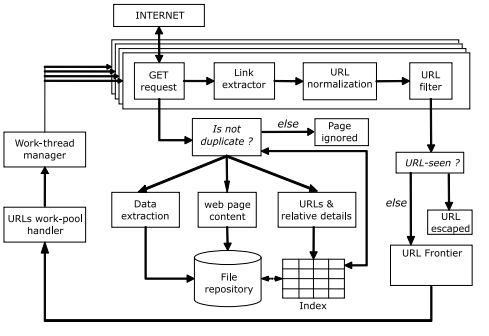
\includegraphics[width=4.5in]{rcrawler-arquitecture.jpg}
  \caption{Rcrawler - Arquitectura y componentes principales de Rcrawler}
  \label{img:rcrawler - arquitectura y componentes principales de rcrawler}
\end{figure}

En primer lugar, el rastreador pone en marcha el entorno de trabajo, es decir, la estructura del índice, 
el repositorio de documentos web y los nodos del clúster para la computación en paralelo. Una vez puesto 
en marcha el entorno de trabajo, se procede con el rastreo el cual es realizado por múltiples hilos de 
trabajo. Por otro lado, el componente \emph{work-pool-handler} prepara un \emph{pool} de URL's para procesar 
en paralelo, donde cada nodo ejecuta las siguientes funciones para cada URL:

\begin{enumerate}
  \item Descargar el documento correspondiente y su cabecera HTTP mediante una petición GET.
  \item Analizar y extraer todos los enlaces contenidos en el documento.
  \item Proceder a la canonización y normalización de URL's.
  \item Aplicar un filtro de URL's, manteniendo sólo aquellas que coincidan con la configuración 
  proporcionada por el usuario, el tipo de archivo y las URL's específicas del dominio.
\end{enumerate}

Tras la descarga del documento a través de la petición GET, se determina si este ya ha sido analizado 
previamente. En caso de que el documento no esté duplicado se procede con el rastreo y la extracción de
datos, con el objetivo de indexar y almacenar los documentos encontrados.

Como resultado, para cada URL cada nodo devuelve su documento HTML, los detalles de la cabecera HTTP y la 
lista de enlaces externos descubiertos. La función \emph{URL-seen} comprueba si la URL ya ha sido procesada.

\subsection{htm2txt}
\label{subsec:htm2txt}

Otro de los paquetes propios de R que se encargan de realizar \emph{web scraping} es \textbf{htm2txt} 
\cite{htm2txt-cran}. Convierte un documento html en textos simples eliminando todas las etiquetas html. 
Este paquete utiliza expresiones regulares para eliminar las etiquetas html. También ofrece las funciones 
\emph{gettxt()} y \emph{browse()}, que permiten obtener o navegar por los textos de una determinada página 
web.

El uso de estas expresiones regulares se hacen notar durante la limpieza del texto extraído, donde la
función \emph{gsub} toma una notable relevancia. Una vez el texto ha sido 'limpiado' se retorna el mismo.

\subsection{scrapeR}
\label{subsec:scraper}

\textbf{scrapeR} \cite{scraper-cran} es otro paquete software que pretende hacer \emph{web scraping} sobre 
documentos basados en la web. El paquete en sí es bastante simple, pues consta de una única función 
encargada de la obtención y creación del árbol DOM para su posterior iteración.

Puesto que no dispone de funciones propias de recorrido del DOM, \textbf{scrapeR} recurre a funciones y
métodos del paquete \emph{XML} para realizar su labor. Esto tiene una ventaja significativa, y es que
permite ejecutar la petición de varias URL's de forma paralela.

\subsection{RSelenium}
\label{subsec:rselenium}

\textbf{RSelenium} \cite{rselenium-cran} es un paquete que tiene como objetivo facilitar la conexión a un 
servidor de Selenium. Además de \emph{web scraping}, \textbf{RSelenium} también permite hacer pruebas de 
unidad y de regresión en las aplicaciones web que se desarrollen utilizando un gran rango de navegadores 
y de sistemas operativos \cite{tfg-daniel-francisco-lopez}. Gracias a esto permite realizar entre otras 
las siguientes tareas:

\begin{enumerate}
  \item Navegar a través de cualquier documento HTML.
  \item Acceder a los elementos del DOM utilizando selectores de id, de clase, de nombre de etiqueta, 
  selectores \emph{XPath} o CSS.
  \item Enviar eventos de teclado y de ratón a los elementos de la página que se determinen.
  \item Inyectar JavaScript en la página.
  \item Utilizar marcos y ventanas diferenciadas.
\end{enumerate}

A modo de anécdota, cabe destacar que mediante el uso de \textbf{RSelenium} es posible automatizar los
navegadores tanto de forma local como remota. Permite manejar un navegador web nativamente como lo haría
un usuario, lo que supone un salto adelante en términos de automatización del \emph{web scraping}.

\section{Paquetes descartados para el proceso de evaluación}
\label{sec:paquetes descartados para el proceso de evaluacion}

A lo largo de las secciones \ref{sec:bibliotecas de python encontradas durante el proceso de busqueda} y
\ref{sec:paquetes de r encontrados durante el proceso de busqueda} se han introducido y desarrollado
aquellas herramientas de \emph{web scraping} más comunes en el entorno de programación. Con el punto de 
mira en los siguientes capítulos, se pretende enumerar aquellos paquetes descartados para el proceso de 
evaluación.

Ya sea por la simpleza de su heurística, por la similitud con otras herramientas, o por la dificultad en 
la instalación y uso de las mismas, las bibliotecas seleccionadas para el descarte son las siguientes:

\begin{itemize}
  \item \textbf{Dragnet}: Uno de los principales motivos por el que Dragnet a sido descartado es por su 
  complejidad en la instalación. La necesidad de un Docker hace que la mayoría de usuarios no programadores 
  hagan uso de otras herramientas en su lugar.
  \item \textbf{news-please}: El descarte de \textbf{news-please} tiene que ver con el uso de otras
  herramientas para el proceso de \emph{web scraping}. La ausencia de heurística propia y el empleo de otros 
  algoritmos como \textbf{Readability} hace que la evaluación de \textbf{news-please} no tenga sentido.
  \item \textbf{Libextract}: Durante el desarrollo de la herramienta de evaluación, se ha detectado que en
  este caso no se cumplían los requisitos mínimos para la misma. La extracción resultaba errónea para
  ciertos documentos HTML.
  \item \textbf{Newspaper3k}: Tal y como se ha indicado en la sinopsis, el algoritmo emplea gran parte de
  la heurística de \textbf{Goose3} para la extracción de contenido. A falta de heurística propia no tendría
  sentido realizar una evolución del mismo.
  \item \textbf{scrapeR}: La sencillez de la herramienta, y su falta de heurística hace que el descarte 
  de la misma sea necesario. Su única función necesita herramientas \emph{XPath} para la búsqueda de 
  información a través del DOM.
  \item \textbf{RSelenium}: Ademas del necesario emplea de un Docker para su uso, al igual que 
  \textbf{scrapeR}, \textbf{RSelenium} carece de heurística propia, ya que para la extracción de texto 
  emplea expresiones \emph{XPath} y selectores CSS únicamente.
\end{itemize}

Por último, es notable la falta de algoritmos de R en la herramienta de evaluación. Durante el proceso de
búsqueda e investigación, la mayoría de ellos no poseen ni siquiera heurística. Trabajar unicamente a 
partir de un analizador y expresiones \emph{XPath}, hace que la evaluación de los mismos no tenga sentido 
alguno.




\chapter{Selección de variables de análisis y proceso de estudio}
\label{cha:seleccion de variables de analisis y proceso de estudio}

Tras la sinopsis de herramientas de \emph{web scraping} de código abierto, se pretende realizar una 
introducción al proceso de evaluación de las mismas. El capítulo se dividirá en tres secciones claramente 
diferenciadas las cuales se especifican con más detalle a continuación:

\begin{enumerate}
  \item En primer lugar se realiza una introducción sobre el proceso de evaluación a realizar. ¿Cuáles
  son los aspectos más importantes en la evaluación de herramientas de minería web? ¿Es posible realizar 
  una valoración objetiva entre bibliotecas de diferentes lenguajes de programación?
  \item La segunda sección trata sobre el proceso de comparación, así como una introducción al código
  desarrollado para este. El proceso de tokenización y la creación/comparación de n-gramas o bloques son 
  algunos de los aspectos a destacar. ¿Cuál es el tamaño óptimo de cada n-grama o bloque? ¿Cómo se determina 
  si la extracción ha sido exitosa?
  \item Por último, se especifican las variables de comparación y los test preparados de cada algoritmo.
  Se determina el proceso seguido para calcular la precisión, velocidad de extracción, uso de memoria
  y demás características de cada algoritmo.
\end{enumerate}

Cabe destacar que la evaluación será conjunta, las herramientas de los diferentes lenguajes de programación 
serán sometidas a los mismos test con el fin de ver aquellas bibliotecas o paquetes más involucrados en el 
proceso de minado web. 

A lo largo del capítulo será posible comprobar en los diferentes fragmentos de código como se ha realizado
la integración de las diversas herramientas, y sobre como es posible construir una valoración objetiva para
cualquier herramienta de minado web desarrollada sobre cualquier lenguaje de programación convencional.

\section{Introducción al proceso de evaluación}
\label{sec:introduccion al proceso de evaluacion}

Cuando cualquier usuario entra en un sitio web lo que busca es obtener la información requerida lo más
rápido y preciso posible. La calidad del texto extraído es prioritaria, para ello el uso de heurísticas o
la eliminación de contenido \emph{boilerplate} es crucial en cualquier algoritmo de \emph{web scraping}.

Muchos de los algoritmos descartados para el proceso de evaluación como \textbf{scrapeR}, o ni si quiera 
mencionados en la sinopsis de paquetes como \textbf{selectr} \cite{selectr}, emplean únicamente expresiones 
regulares para la extracción de contenido. Esto provoca que la extracción de texto no sea 'limpia', puesto 
que siempre van a existir resultados donde se extraiga contenido no deseado.

El objetivo de este proyecto concierne la evaluación del proceso heurístico de las diferentes herramientas
de minado web. La inclusión de algoritmos que emplean únicamente expresiones \emph{XPath} o selectores CSS 
no tiene sentido para la herramienta desarrollada, pues cualquier analizador de los ya mencionados en el
apéndice \ref{cha:analizadores empleados en los paquetes de web scraping} podría realizar el mismo trabajo.

\subsection{Aspectos generales a considerar}
\label{subsec:aspectos generales a considerar}

La gran mayoría de los \emph{web scrapers} son capaces de extraer fragmentos de información de un sitio
web, ya sea el precio de un determinado producto en venta, el autor de un ensayo o el resultado de un 
partido de fútbol. Pero además, se espera que estas herramientas de minado puedan ser una solución fiable 
y de calidad con respecto a la extracción tradicional, ¿es posible medir de algún modo la calidad del texto 
extraído de estas herramientas?

La respuesta es si, y para ello, los algoritmos se centrarán en la extracción de artículos de prensa en su
mayoría, con el objetivo de que estos sean comparados con un texto base. Se define como texto base aquellos 
fragmentos de texto principal de cualquier sitio web que el usuario visualizaría al entrar. Se muestra en 
la figura \ref{img:estructura generica del proceso de evaluacion} la estructura general del proceso de 
evaluación.

\begin{figure}[tphb]
  \centering
  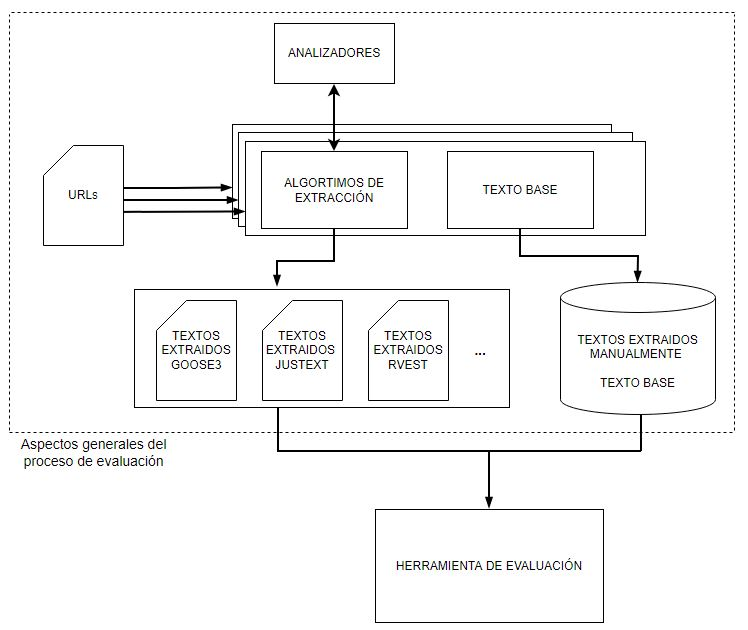
\includegraphics[width=5in]{estructura-generica-proceso-evaluacion.jpg}
  \caption{Estructura genérica del proceso de evaluación}
  \label{img:estructura generica del proceso de evaluacion}
\end{figure}

Tanto los textos obtenidos por los algoritmos de \emph{web scraping}, como los textos producidos por la 
extracción manual, se almacenan de forma ordenada en archivos JSON. Esto se hace con el objetivo de que su 
acceso sea sencillo para cualquier lenguaje de programación.

\subsection{Cuerpo principal del sitio web como objetivo de la evaluación}
\label{subsec:cuerpo principal del sitio web como objetivo de la evaluacion}

Como ya se ha mencionado anteriormente, una de las características más importantes de un \emph{web scraper}
es la capacidad de extraer de texto de calidad. Por lo tanto, comparar el texto extraído de diferentes
algoritmos será el cometido de la herramienta de evaluación. Ahora la principal pregunta es, ¿qué fragmentos
de texto son considerados como principales?

Imaginemos un artículo web de noticias tradicional o una entrada de blog, algo parecido a lo mostrado en
la figura \ref{img:articulo web tradicional}, del que se pretende extraer
información de valor. En la imagen se reflejan varias secciones claramente diferenciadas, anuncios de
contenidos relacionados, información de autor e incluso elementos de navegación.

\begin{figure}[tphb]
  \centering
  
\includegraphics[width=6in]{pagina-web.jpeg}
  \caption{Artículo web tradicional}
  \label{img:articulo web tradicional}
\end{figure}

La tarea de extracción puede parecer sencilla, pero dependiendo del sitio web puede ser sorprendentemente
complicada y llena de matices \cite{boilerplate-removal}. La selección del cuerpo principal del sitio web 
será el objetivo de cada algoritmo. Para conseguir un cuerpo de artículo no solo será necesario saber dónde 
empieza o termina este, también se deberán conocer las partes a excluir. 

Con el fin de la que la evaluación sea lo más justa posible, se debe definir qué compone el cuerpo del
artículo, y estar seguros de que todas las herramientas siguen los mismos objetivos. El principio subyacente 
es que el cuerpo del artículo debe ser un texto limpio, sin campos adicionales, elementos de navegación o 
anuncios. En la siguiente lista se determina el conjunto de elementos o secciones de un sitio web no 
contemplados en la evaluación:

\begin{itemize}
  \item Campos de información sobre autor/es, fechas de publicación, palabras clave o títulos de imágenes 
  y vídeos.
  \item Botones para compartir y sugerencias para compartir un artículo, artículos relacionados, enlaces 
  'leer a continuación', 'recomendado para usted'...
  \item Comentarios e interfaz de usuario relacionada con los mismos. Elementos de navegación propios del
  sitio web.
  \item Elementos de control alrededor de las imágenes que producen texto innecesario, número de imágenes
  en una galería, botones superpuestos a una imagen/vídeo...
  \item Código JavaScript. Aunque esta no sea una sección específica de un sitio web, muchas herramientas
  extraen estos fragmentos de código pensado que pertenece como parte del contenido principal del propio 
  artículo.
\end{itemize}

Se muestra a continuación la lista de elementos que serán extraídos por las diferentes herramientas como
parte del contenido principal, ademas del propio contenido principal.

\begin{itemize}
  \item Título principal de artículo.
  \item Enlaces para leer con más detalle, a la fuente u otros contenidos directamente relacionados. Estos 
  enlaces pueden requerir un conocimiento mucho más profundo y complejo del contenido principal del sitio 
  web.
  \item Avisos de copyright.
\end{itemize}

En definitiva, todo fragmento que pueda ser extraído y comparado con el original y del que se puedan obtener 
conclusiones firmes, será incluido como parte del contenido principal. Véase la figura 
\ref{img:contenido boilerplate de un articulo web tradicional} en la que se determinan las secciones 
descartadas y definidas como contenido \emph{boilerplate} o 'basura'.

\begin{figure}[tphb]
  \centering
  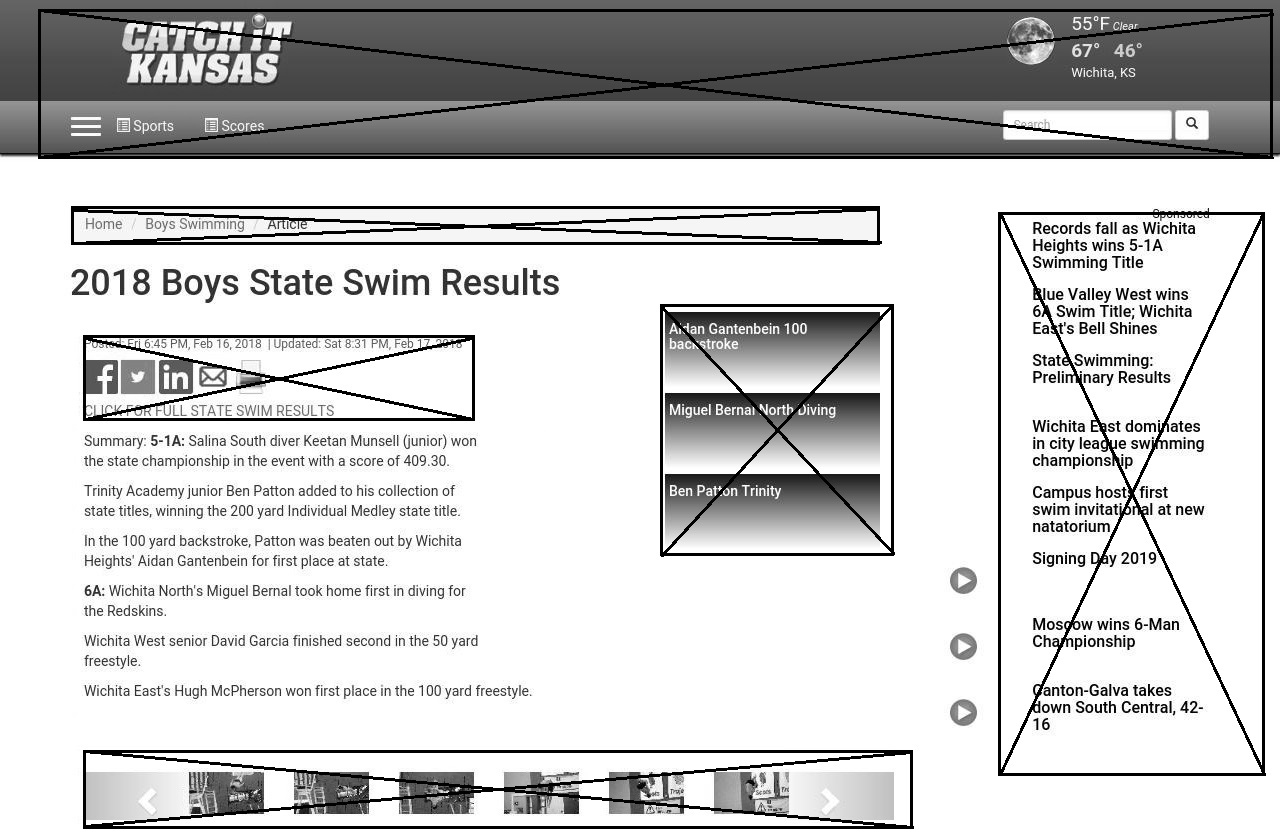
\includegraphics[width=6.1in]{pagina-web2.jpeg}
  \caption{Contenido \emph{boilerplate} de un artículo web tradicional}
  \label{img:contenido boilerplate de un articulo web tradicional}
\end{figure}

\subsection{Recopilación del conjunto de datos}
\label{subsec:recopilacion del conjunto de datos}

Una vez definido en que consiste el cuerpo principal de cada artículo, el siguiente paso consiste en la
recolección del conjunto de datos de prueba para la herramienta. Se pretende que este conjunto sea diverso, 
representativo e imparcial. Es por ello que en el \emph{dataset} no solo se compone artículos de noticias 
relevantes, también hay un conjunto muy variado de artículos no informativos como entradas de blog, 
comunicados de prensa...

El proceso de recolección del conjunto de datos consiste en tomar una muestra aleatoria del millón de
sitios web escritos en inglés. Para cada sitio, se comprueba si contiene algún artículo, en cuyo caso, se
añaden dos de ellos al azar. En una primera instancia, el conjunto que compone el \emph{dataset} suponía
cerca de 200 sitios web listos para analizar.

Antes de comenzar con el proceso de evaluación se deben asegurar una serie de conceptos relacionados con
posibles errores de acceso, análisis o extracción de la información de algunas de las páginas incluidas:

\begin{enumerate}
  \item Se debe asegurar que las páginas no cambian durante el análisis. Minimizar las posibilidades de 
  obtener un artículo actualizado durante la extracción.
  \item Se deben excluir aquellas páginas que las herramientas no sean capaces de descargar.
  \item Se deben descartar aquellas paginas cuyo contenido no sea explícitamente escrito en inglés.
\end{enumerate}

Tras tener en cuenta todas estas consideraciones, el grupo inicial de 200 páginas se redujo a 101 casos
listos para el análisis. Aún realizada la reducción, el \emph{dataset} es lo suficientemente amplio como
para sacar conclusiones claras de los algoritmos a analizar.

Por último, como ya se ha mencionado anteriormente, tanto la información extraída de forma manual, como
aquella extraída por los algoritmos de minado web, es almacenada en archivos JSON. Esto hace mucho más
cómodo el análisis, pues el acceso a cada texto es mucho más sencillo. Se muestra a continuación un ejemplo
de como se almacenan los diferentes textos extraídos por \textbf{BeautifulSoup}.

\begin{Schunk}
  \begin{Soutput}
  {
    "0000test": {
        "texto": "Nadal keeps Spain alive against Russia in Davis Cup Finals..."
    },
    ...
    "0100test": {
        "texto": "CNN - Breaking News, Latest News and Videos CNN | 11/25/2021..."
    }
  }
  \end{Soutput}
\end{Schunk}

De la misma forma se almacenan los textos extraídos de forma manual. En este caso, se guarda información
adicional del sitio web. Como se puede observar, el orden de almacenamiento es clave, pues de él depende
que el análisis sea correcto.

\begin{Schunk}
  \begin{Soutput}
  {
    "0000test": {
        "texto": "MADRID — Rafael Nadal kept Spain’s hopes alive, then Marcel...",
        "url": "https://www.sportsnet.ca/tennis/..."
    },
    ...
    "0100test": {
      "texto": "Groups of thieves target two high-end stores in California...",
      "url": "http://lite.cnn.com/en/article/..."
    }
  }
  \end{Soutput}
\end{Schunk}

Esta forma de almacenamiento es aplicada a todos los algoritmos de minado, no solo a aquellos desarrollados
en Python, las herramientas codificadas en R también lo aplican. Esto permite incluir en la evaluación a
cualquier algoritmo de minado web desarrollado sobre un lenguaje de programación que permita trabajar con
documentos JSON.

\section{Análisis de la herramienta de evaluación}
\label{sec:analisis de la herramienta de evaluacion}

Una vez se dispone del \emph{dataset} al completo, el objetivo es comparar cada uno de los textos obtenidos
por las herramientas de extracción con el texto base. La exposición de las diferentes soluciones aportadas
será clave para comprender el resultado final.

Uno de los aspectos fundamentales de la herramienta de evaluación es su heurística. Se debe pensar en un
algoritmo que sea capaz de comparar diferentes tipos de textos minimizando la probabilidad de fallo. A lo
largo de la sección se mostrará como el proceso no es sencillo, pues muchos algoritmos de extracción
presentan diferentes soluciones a un mismo problema.

\begin{figure}[tphb]
  \centering
  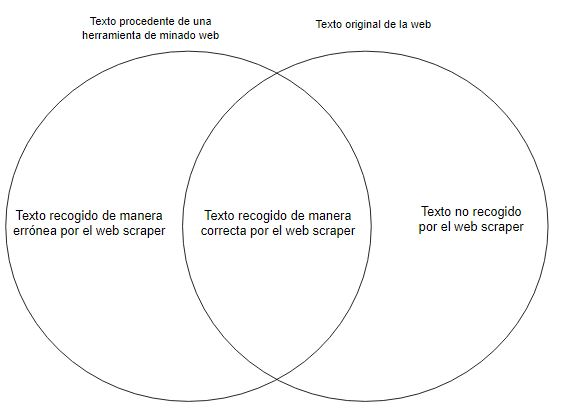
\includegraphics[width=5in]{diagrama-venn.jpg}
  \caption{Diagrama de Venn: Texto base vs texto extraído}
  \label{img:diagrama venn: texto base vs texto extraido}
\end{figure}

La principal preocupación subyace por la forma en la que los diferentes algoritmos consideran como parte
de contenido principal de un sitio web. En algunas ocasiones es posible configurar la manera de extracción
de los mismos, pero en otra no. Es por ello que se debe pensar en un método lo suficientemente justo como
para comparar múltiples textos de diversas procedencias que pueden ser ligeramente diferentes.

\subsection{Aspectos específicos a considerar}
\label{subsec:aspectos especificos a considerar}

En la figura \ref{img:estructura generica del proceso de evaluacion} se definía de forma genérica como se
gestionaba la información recogida por los diferentes algoritmos de \emph{web scraping}. Veamos ahora como
se trata y se compara dicha información con la extraída manualmente, con el objetivo de conocer aquellos
algoritmos que más se acercan a un resultado real.

\begin{figure}[tphb]
  \centering
  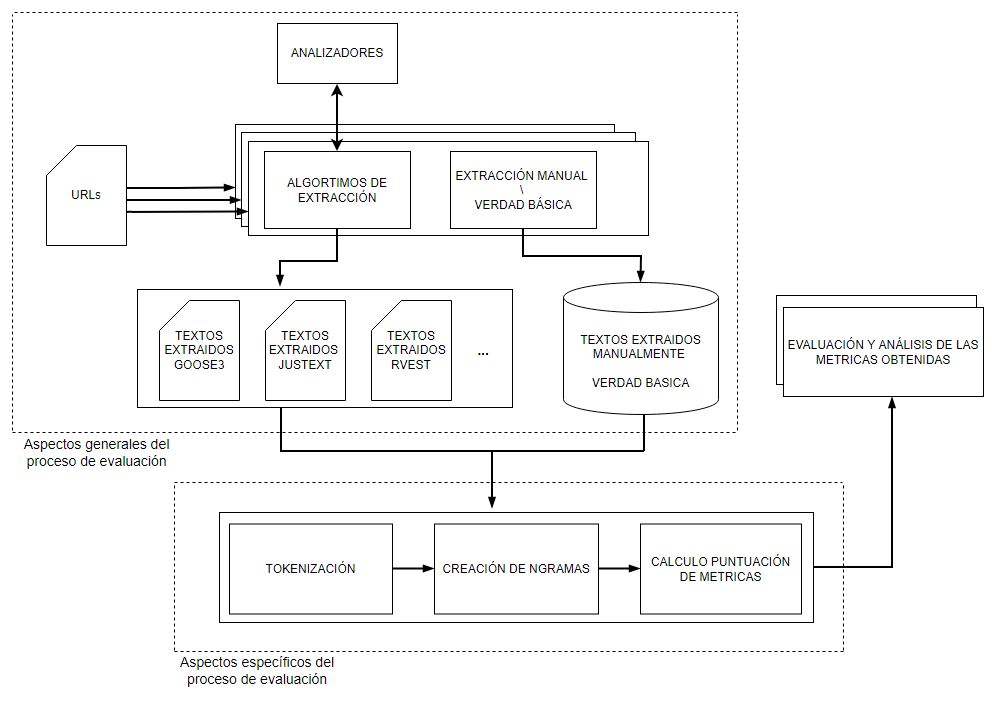
\includegraphics[width=7.1in]{estructura-especifica-proceso-evaluacion.jpg}
  \caption{Estructura especifica del proceso de evaluación}
  \label{img:estructura específica del proceso de evaluacion}
\end{figure}

Se puede observar en la figura \ref{img:estructura específica del proceso de evaluacion} la solución
adoptada por la herramienta de evaluación. Tras la obtención de texto base y texto extraído, se pretende
realizar un proceso de tokenización y creación de n-gramas, clave a la hora de realizar el posterior cálculo
de métricas. En cuanto a la evaluación y análisis de métricas obtenidas, se abordará en el próximo capítulo.

\subsection{Heurística basada en n-gramas}
\label{subsec:heuristica basada en n-gramas}

A lo largo de la sección se aborda el problema de comparar diferentes fragmentos de texto. Se presentan
diferentes soluciones, una de ellas podría ser la comparación de palabras en la misma posición, otra podría
ser la búsqueda de palabras pertenecientes a ambos textos. Veamos porque la división en n-gramas es un
buen método para este propósito.

\subsubsection{Comparación de texto empleando el método palabra por posición}
\label{subsubsec:comparacion de textos empleando el metodo palabra por posicion}

Imaginemos que se disponen dos textos a comparar como los siguientes. El primero de ellos se considera como
texto base, pues ha sido obtenido de forma manual del propio sitio web. El segundo surge como resultado 
de la ejecución de cualquiera de las herramientas de \emph{web scraping} expuestas en el capítulo anterior.

\begin{Schunk}
  \begin{Soutput}
      MADRID — Top-ranked Rafael Nadal has arrived in Madrid to
      lead Spain in the new-look Davis Cup Finals.\n\n\"It’s a
      new competition and we must be focused,\" Nadal said Sunday.

      MADRID \u2014 Top-ranked Rafael Nadal has arrived in Madrid to 
      lead Spain in the new-look Davis Cup Finals.\"It\u2019s a 
      new competition and we must be focused,\" Nadal said Sunday.
  \end{Soutput}
\end{Schunk}

Veamos el funcionamiento de los diferentes métodos de comparación pensados. En primer lugar, se aplica la
comparación palabra por posición, donde se prepara un fragmento de código que recorra ambos textos al mismo
tiempo y determine si las palabras dispuestas en la misma posición son idénticas.

\begin{figure}[tphb]
  \centering
  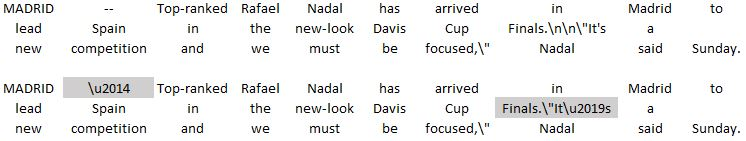
\includegraphics[width=6.5in]{text-comparison1.jpg}
  \caption{Comparación de textos empleando el método palabra por posición}
  \label{img:comparacion de textos empleando el metodo palabra por posicion}
\end{figure}

Como se muestra en la figura \ref{img:comparacion de textos empleando el metodo palabra por posicion} la 
comparación no ha sido tan desastrosa como se esperaba. Los únicos errores han sido producidos por espacios 
en blanco y caracteres Unicode que la herramienta de minado web no ha sido capaz de detectar.

El problema con esta solución viene cuando la disposición de los mismos no es exacta, o incluso cuando 
ambos fragmentos no tienen el mismo tamaño. Imaginemos que la herramienta de minado no ha sido capaz de 
detectar la palabra \textbf{MADRID} como parte del contenido principal. En este caso, ninguna palabra 
coincidiría con la original pues las posiciones no están dispuestas del mismo modo.

\begin{figure}[tphb]
  \centering
  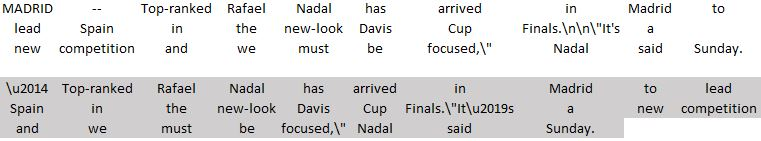
\includegraphics[width=6.5in]{text-comparison2.jpg}
  \caption{Comparación de textos empleando el método palabra por posición}
  \label{img:comparacion de textos empleando el metodo palabra por posicion p2}
\end{figure}

Esta forma de comparación no funcionaria, y menos en artículos donde los fragmentos de textos son amplios
y las posibilidades de fallo aumentan. Además, el \emph{dataset} es de gran volumen por lo que la posibilidad 
de que existan fragmentos de texto con disposiciones totalmente distintas a la original tiene una alta 
probabilidad.

\subsubsection{Comparación de texto empleando el método palabra por detección}
\label{subsubsec:comparacion de textos empleando el metodo palabra por deteccion}

Es necesario encontrar entonces una nueva heurística que minimice la probabilidad de fallo, donde la 
posición de cada palabra no sea un aspecto a tener en cuenta. Una solución podría darse con el recorrido 
de uno de los fragmentos de texto, donde se busquen palabras coincidentes con el otro. Se selecciona una 
palabra pivote, por ejemplo \textbf{Spain}, y se recorre el segundo texto hasta encontrar la palabra 
indicada.

\begin{figure}[tphb]
  \centering
  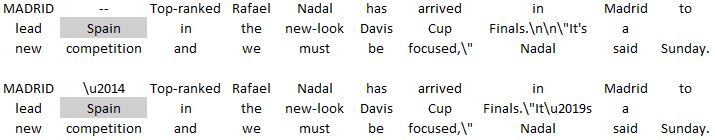
\includegraphics[width=6.5in]{text-comparison3.jpg}
  \caption{Comparación de textos empleando el método palabra por detección}
  \label{img:comparacion de textos empleando el metodo palabra por deteccion}
\end{figure}

En realidad, si se realiza un análisis profundo sobre esta solución, surgen nuevas problemáticas. ¿Qué
ocurriría si apareciesen dos palabras idénticas sobre el mismo texto? Imaginemos que durante el recorrido
del primer texto, se debe analizar una palabra pivote repetida varias veces a lo largo del segundo texto. 
La heurística anterior no sería correcta, veamos un ejemplo.

Comienza el algoritmo seleccionando pivotes y realizando la heurística correspondiente para cada uno, 
primero con \textbf{MADRID}, luego con \textbf{'--'}, y así sucesivamente hasta llegar a \textbf{Nadal} 
que es el que nos interesa en este ejemplo. Se recorre el segundo fragmento buscado dicha palabra y se 
encuentran dos apariciones de la misma. Para ambas apariciones se calcula y se suma una puntuación 
determinada.

\begin{figure}[tphb]
  \centering
  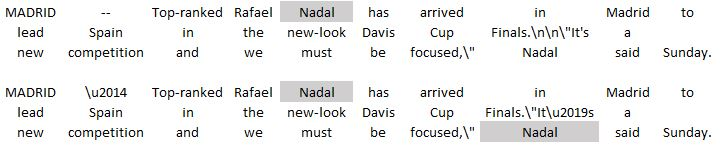
\includegraphics[width=6.5in]{text-comparison4.jpg}
  \caption{Comparación de textos empleando el método palabra por detección}
  \label{img:comparacion de textos empleando el metodo palabra por deteccion p2}
\end{figure}

El algoritmo sigue realizando el bucle y nuevamente emplea la palabra \textbf{Nadal} como pivote, pero en
este caso en su segunda aparición. Se volvería a efectuar un calculo y la posterior suma de su puntuación.
La implementación de esta heurística forzaría un resultado irreal, pues este error se acrecentaría sobre
\emph{datasets} extensos que contengan fragmentos de texto prolongados, como es el caso.

\begin{figure}[tphb]
  \centering
  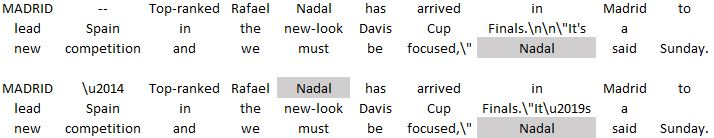
\includegraphics[width=6.5in]{text-comparison5.jpg}
  \caption{Comparación de textos empleando el método palabra por detección}
  \label{img:comparacion de textos empleando el metodo palabra por deteccion p3}
\end{figure}

\subsubsection{Comparación de texto empleando la creacion de n-gramas}
\label{subsubsec:comparacion de textos empleando la creacion de n-gramas}

Se debe pensar entonces en una nueva heurística que nuevamente minimice la probabilidad de fallo, la cual
tenga en cuenta que la posición de cada palabra debe ser irrelevante y que cuide la posible repetición de
palabras. Se utilizan bloques como estructuras de datos, veamos como funciona.

Los bloques o n-gramas se consideran conjuntos de secuencias alfanuméricas, en las que se descartan los
espacios en blanco y se separan los signos de puntuación \cite{ngrams-thesis}. Esto funciona bien en la 
mayoría de los casos, ya que normalmente el texto a excluir se encuentra en bloques separados por nuevas 
líneas o espacios en blanco. Siguiendo con el ejemplo anterior, la división de texto en n-gramas donde 
\emph{n = 3} sería:

\begin{figure}[tphb]
  \centering
  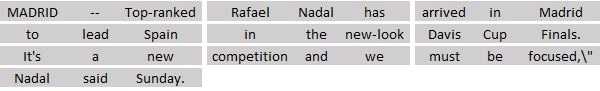
\includegraphics[width=6in]{text-comparison6.jpg}
  \caption{Creación de n-gramas}
  \label{img:creacion de n-gramas}
\end{figure}

El objetivo ahora es separar ambos textos en n-gramas de tamaño \emph{n} y realizar la comparación entre
ellos. La posición ya no es relevante pues la comparación no se va a ejecutar en torno a la posición de cada
n-grama. Además, la repetición de n-gramas no es preocupante pues existe una baja probabilidad de que esto
ocurra a lo largo del texto.

\begin{figure}[tphb]
  \centering
  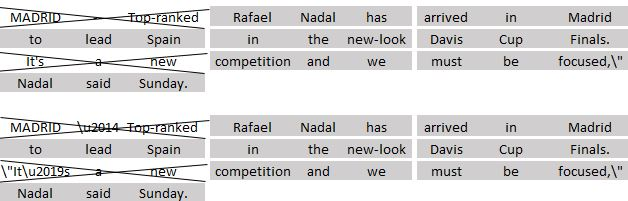
\includegraphics[width=6in]{text-comparison7.jpg}
  \caption{Comparación de textos empleando n-gramas}
  \label{img:comparacion de textos empleando n-gramas p2}
\end{figure}

El algoritmo procede del mismo modo que antes, se selecciona un n-grama pivote y se buscan n-gramas
coincidentes en el texto extraído. Tras el recorrido completo del texto se determina una cierta puntuación.
En la figura \ref{img:comparacion de textos empleando n-gramas p2} se muestra el resultado de ejecución
del algoritmo.

Si observamos de nuevo la figura anterior, los n-gramas en séptima y primera posición del texto base no 
coincide con los n-gramas del texto extraído, a pesar de que la mayor parte de las palabras sí que son 
coincidentes. Es posible realizar una mejora dividiendo el texto en el mayor número de n-gramas posibles. 
Este aumento de divisiones se efectúa con el objetivo de recuperar la mayor cantidad de palabras mejorando 
así la precisión de la herramienta desarrollada.

\begin{codefloat}
  \inputencoding{latin1}
  \lstinputlisting[style=CppExample, showstringspaces=false]{scripts/evaluacion-tokenizar.py}
  \inputencoding{utf8}
  \caption{Proceso de tokenización}
  \label{cod:proceso de tokenizacion}
\end{codefloat}

En los fragmentos de código \ref{cod:proceso de tokenizacion} y
\ref{cod:creacion de n-gramas a partir de los tokens resultantes} se muestra el proceso de tokenización y
creación de n-gramas usado en la herramienta de evaluación. Para el desarrollo de la herramienta se ha
decidido emplear n-gramas donde \emph{n = 4} con el objetivo de aumentar la precisión del resultado dado.

\begin{codefloat}
  \inputencoding{latin1}
  \lstinputlisting[style=CppExample, showstringspaces=false]{scripts/evaluacion-ngramas.py}
  \inputencoding{utf8}
  \caption{Creación de n-gramas a partir de los tokens resultantes}
  \label{cod:creacion de n-gramas a partir de los tokens resultantes}
\end{codefloat}

Aplicando esta metodología al ejemplo anterior se obtienen una cantidad bastante mayor de n-gramas. Este
mismo proceso se realiza tanto en el texto base, como en el texto extraído, para poder realizar el cálculo
posterior de la puntuación.

\begin{Schunk}
  \begin{Soutput}
(MADRID -- Top-ranked Rafael), (-- Top-ranked Rafael Nadal), 
(Top-ranked Rafael Nadal has), (Rafael Nadal has arrived), 
(Nadal has arrived in), (has arrived in Madrid), (arrived in Madrid to), 
(in Madrid to lead), (Madrid to lead Spain), (to lead Spain in), 
(lead Spain in the), (Spain in the new-look), (in the new-look Davis), 
(the new-look Davis Cup), (new-look Davis Cup Finals.), (Davis Cup Finals. It’s),
(Cup Finals. It’s a), (Finals. It’s a new), (It’s a new competition),
(a new competition and), (new competition and we), (competition and we must), 
(and we must be), (we must be focused,), (must be focused, Nadal),
(be focused, Nadal said), (focused, Nadal said Sunday.)
  \end{Soutput}
\end{Schunk}

\subsection{Cálculo y puntuación de n-gramas}
\label{subsec:calculo y puntuacion de n-gramas}

Una vez que ambos fragmentos de texto han sido convertidos en n-gramas, se debe realizar el cálculo del
texto extraído para poder conocer la calidad del mismo. Para comprender como se ha desarrollado dicho
cálculo, debemos recordar la figura \ref{img:diagrama venn: texto base vs texto extraido}, donde el 
diagrama expuesto representa los tres posibles tipos de puntuaciones.

Para realizar el cálculo y puntuación de n-gramas, se desarrolla un clasificador binario, encargado de
realizar una división de instancias positivas y negativas:

\begin{itemize}
  \item Positivo: La instancia se clasifica como miembro de la clase que el clasificador está tratando de 
  identificar. Por ejemplo, un clasificador que busque fotos de gatos clasificará las fotos con gatos como 
  positivas cuando sean correctas.
  \item Negativo: La instancia se clasifica como no perteneciente a la clase que se intenta identificar. 
  Por ejemplo, un clasificador que busque fotos de gatos debería clasificar las fotos con perros como 
  negativas.
\end{itemize}

Las bases de las métricas independientes del entorno de ejecución especificadas en la sección
\ref{subsubsec:metricas independientes del entorno de ejecucion}, provienen de los conceptos de 
\textbf{True Positive}, \textbf{False Positive} y \textbf{False Negative}. La tabla 
\ref{tab:ejemplos de instancias positivas y negativas} ilustra estos conceptos, donde se considera el 
valor '1' como una predicción positiva.

\begin{table}[h]
  \begin{center}
  \begin{tabular}{| c | c | c | c |} \hline
  \textbf{Predicción} & \textbf{Valor actual} & \textbf{Tipo} & \textbf{Explicación}\\ \hline
  1 & 1 & True Positive & La predicción coincidió con el valor resultante \\ \hline
  1 & 0 & False Positive & La predicción no coincidió con el valor resultante \\ \hline
  0 & 1 & False Negative & La predicción no coincidió con el valor resultante \\ \hline
  \end{tabular}
  \caption{Ejemplos de instancias positivas y negativas}
  \label{tab:ejemplos de instancias positivas y negativas}
  \end{center}
\end{table}

Una instancia que no se tiene en cuenta en el clasificador desarrollado para el cálculo de métricas es 
\textbf{True Negative}. Esta instancia determinaría la capacidad de la herramienta para clasificar contenido 
que no se ha predicho. Se muestran algunos ejemplos en la tabla \ref{tab:ejemplos de true negative}.

\begin{table}[h]
  \begin{center}
  \begin{tabular}{| c | c | c | c |} \hline
  \textbf{Predicción} & \textbf{Valor actual} & \textbf{Tipo} & \textbf{Explicación}\\ \hline
  0 & 0 & True Negative & La predicción coincidió con el valor resultante \\ \hline
  No Gato & No Gato & True Negative & Se predijo que no había gato y no era un gato \\ \hline
  (Nadal Rafael has) & (Nadal Rafael has) & True Negative & Se predijo n-grama erróneo y era erróneo \\ \hline
  \end{tabular}
  \caption{Ejemplos de True Negative}
  \label{tab:ejemplos de true negative}
  \end{center}
\end{table}

Los n-gramas que coinciden en el texto base y en el texto extraído se conoce como \textbf{True Positives}.
Se muestra en el fragmento de código \ref{cod:calculo de true positives} como se realiza dicho cálculo.

\begin{codefloat}
  \inputencoding{latin1}
  \lstinputlisting[style=CppExample, showstringspaces=false]{scripts/evaluacion-true-positives.py}
  \inputencoding{utf8}
  \caption{Cálculo de true positives}
  \label{cod:calculo de true positives}
\end{codefloat}

Por otro lado, los n-gramas que aparecen en el texto extraído, pero no en el texto base se conoce como 
\textbf{False Positives}. Se muestra en el fragmento de código \ref{cod:calculo de false positives} como 
se realiza dicho cálculo.

\begin{codefloat}
  \inputencoding{latin1}
  \lstinputlisting[style=CppExample, showstringspaces=false]{scripts/evaluacion-false-positives.py}
  \inputencoding{utf8}
  \caption{Cálculo de false positives}
  \label{cod:calculo de false positives}
\end{codefloat}

Por ultimo, los n-gramas que aparecen en el texto base pero no en el texto extraído se conoce como 
\textbf{False Negatives}. Se muestra en el fragmento de código \ref{cod:calculo de false negatives} como 
se realiza dicho cálculo.

\begin{codefloat}
  \inputencoding{latin1}
  \lstinputlisting[style=CppExample, showstringspaces=false]{scripts/evaluacion-false-negatives.py}
  \inputencoding{utf8}
  \caption{Cálculo de false negatives}
  \label{cod:calculo de false negatives}
\end{codefloat}

Una vez conocidas estas tres posibles puntuaciones, lo único que se debe hacer es recorrer el texto base
y texto extraído, haciendo una comparación de n-gramas. El código fragmento de código mostrado en
\ref{cod:calculo de puntuaciones} se encarga de retornar una tupla con las puntuaciones calculadas.

\begin{codefloat}
  \inputencoding{latin1}
  \lstinputlisting[style=CppExample, showstringspaces=false]{scripts/evaluacion-puntuacion.py}
  \inputencoding{utf8}
  \caption{Cálculo de puntuaciones}
  \label{cod:calculo de puntuaciones}
\end{codefloat}

Con el objetivo de esclarecer como funciona el cálculo de la puntuación, se emplea el ejemplo anterior
como sujeto de pruebas. Se muestra a continuación el texto base y extraído convertidos en n-gramas donde 
\emph{n = 4}.

\begin{figure}[tphb]
  \centering
  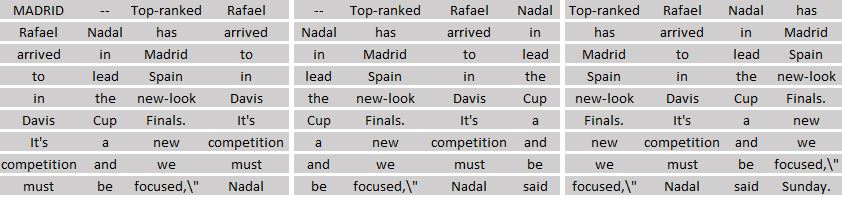
\includegraphics[width=6.3in]{text-comparison8.jpg}
  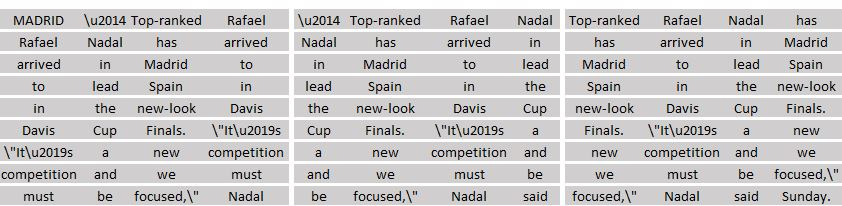
\includegraphics[width=6.3in]{text-comparison9.jpg}
  \caption{Comparación de textos empleando n-gramas mejorados}
  \label{img:comparacion de textos empleando n-gramas mejorados}
\end{figure}

Una vez aplicada la heurística habitual del algoritmo, se procede con el cálculo de la puntuación. Se
realiza el recorrido de n-gramas de ambos textos y se va realizando el cálculo. Se muestran las puntuaciones 
calculadas la matriz de confusión \ref{img:matriz de confusion de las instancias calculadas}.

\begin{figure}[tphb]
  \centering
  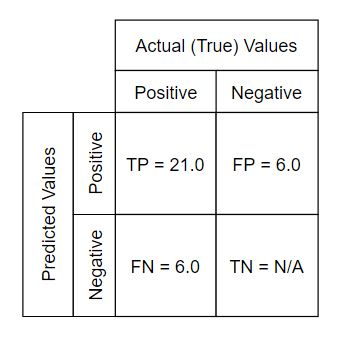
\includegraphics[width=4.5in]{matriz-confusion.jpg}
  \caption{Matriz de confusión de las instancias calculadas}
  \label{img:matriz de confusion de las instancias calculadas}
\end{figure}

Una vez realizado el cálculo de las diferentes instancias, se procede con las métricas. Algunos términos 
básicos son \textbf{Precision}, \textbf{Recall} y \textbf{F1-Score}. Estos términos están relacionados con 
lo bien que funciona un clasificador, en lugar de limitarse a observar la precisión general.

\subsection{Introducción a las métricas de evaluación}
\label{subsec:introduccion a las metricas de evaluacion}

Después de realizar todo el proceso heurístico y el posterior cálculo de puntuaciones, se debe medir como 
de buenos son los diferentes algoritmos de extracción. Se propone efectuar una división de métricas, por 
un lado, se determinarán métricas que dependan del entorno en el que se ejecute el programa, por otro lado,
se definirán otras métricas no dependientes de dicho entorno. 

Es conveniente revisar el apéndice \ref{cha:metricas descartadas del proceso de evaluacion}, donde se 
especifican métricas adicionales que finalmente han sido descartadas. Su descarte, es debido a su poca 
implicación en la evaluación o por el reemplazo de otras métricas más desarrolladas.

\subsubsection{Métricas independientes del entorno de ejecución}
\label{subsubsec:metricas independientes del entorno de ejecucion}

En esta sección, se determinan las diferentes métricas que definirán la calidad de extracción de cada 
algoritmo. Se definen como métricas independientes del entorno, porque no dependen del medio de ejecución, 
ni del lenguaje de programación usado para dicho procedimiento.

En la figura \ref{img:jerarquia de metricas} se muestra la jerarquía existente entre el cálculo de instancias
y métricas. A primera vista, es una red un poco desordenada. Las métricas forman una jerarquía que comienza
con las negativas/positivas, y que llega hasta la puntuación F1 para unirlas todas. Estas métricas son 
dependientes de las instancias previamente calculadas.

\begin{figure}[tphb]
  \centering
  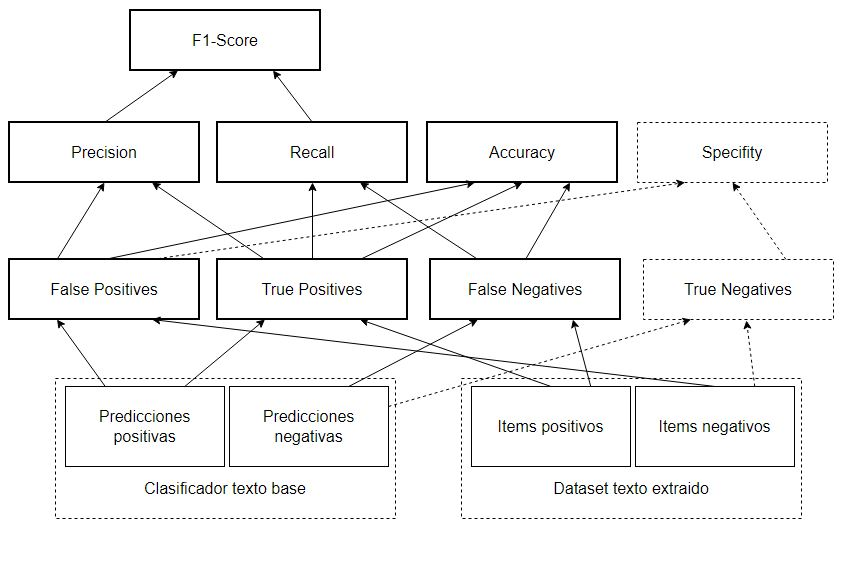
\includegraphics[width=6.5in]{estructura-metricas.jpg}
  \caption{Jerarquía de métricas}
  \label{img:jerarquia de metricas}
\end{figure}

La primera métrica se conoce como \emph{precision}, y mide el número de predicciones positivas realizadas
que son correctas. En otras palabras, mide la eficacia de los sistemas para excluir contenido
\emph{boilerplate} de un sitio web. A continuación se determina tanto la formula para su cálculo, como el
fragmento de código incluido en la herramienta de evaluación.

\begin{equation*}
  Precision = \frac{True\;Positives}{True\;Positives + False\;Positives} = 
  \frac{N.\;of\;Correctly\;Predicted\;Positive\;Instances}{N.\;of\;Total\;Positives\;Predictions\;you\;Made}
\end{equation*}

\begin{codefloat}
  \inputencoding{latin1}
  \lstinputlisting[style=CppExample, showstringspaces=false]{scripts/evaluacion-precision.py}
  \inputencoding{utf8}
  \caption{Cálculo de la métrica \emph{precision}}
  \label{cod:calculo de la metrica precision}
\end{codefloat}

Otra de las métricas obligadas a calcular es lo que se conoce como \emph{recall}. Esta característica mide
el número de casos positivos que el clasificador predijo correctamente, sobre todos los casos positivos del
\emph{dataset}. A veces también se denomina \emph{sensitivity}. En términos generales, mide la eficacia de
los sistemas para captar las partes deseadas del cuerpo del artículo. En el fragmento de código
\ref{cod:calculo de la metrica recall} se muestra como se realiza el cálculo.

\begin{equation*}
  Recall = \frac{True\;Positives}{True\;Positives + False\;Negatives} = 
  \frac{N.\;of\;Correctly\;Predicted\;Positive\;Instances}{N.\;of\;Total\;Positives\;Intances\;in\;the\;Dataset}
\end{equation*}

\begin{codefloat}
  \inputencoding{latin1}
  \lstinputlisting[style=CppExample, showstringspaces=false]{scripts/evaluacion-recall.py}
  \inputencoding{utf8}
  \caption{Cálculo de la métrica \emph{recall}}
  \label{cod:calculo de la metrica recall}
\end{codefloat}

Tanto la \emph{precision} como \emph{recall} son métricas importantes de analizar, puesto que miden como
de bien diferencian el contenido importante del contenido \emph{boilerplate} los diferentes algoritmos de
\emph{web scraping}. Estas métricas definen la manera en la que los algoritmos siguen lo especificado en
la sección \ref{subsec:cuerpo principal del sitio web como objetivo de la evaluacion}.

Combinando ambas métricas es posible determinar la calidad en general de la extracción. Esta característica
se denomina F1, y funciona bien en los casos en los que los conjuntos de datos están desequilibrados,
ya que requiere que tanto las métricas de \emph{precision} como \emph{recall} tengan un valor razonable.

\begin{equation*}
  F1 = 2 * \frac{precision * recall}{precision + recall}
\end{equation*}

Por último, se realiza el cálculo de lo que se conoce como \emph{accuracy}, la cual mide la proporción de
predicciones correctas sobre el número total de predicciones. A continuación se muestra tanto la fórmula
de cálculo, como su implementación en el entorno de evaluación.

\begin{equation*}
  Accuracy = \frac{True\;Positives}{True\;Positives + False\;Negatives + False\;Positives} = 
  \frac{N.\;of\;Correct\;Predictions}{N.\;of\;All\;Predictions}
\end{equation*}

\begin{codefloat}
  \inputencoding{latin1}
  \lstinputlisting[style=CppExample, showstringspaces=false]{scripts/evaluacion-accuracy.py}
  \inputencoding{utf8}
  \caption{Cálculo de la métrica \emph{accuracy}}
  \label{cod:calculo de la metrica accuracy}
\end{codefloat}

\subsubsection{Métricas dependientes del entorno de ejecución}
\label{subsubsec:metricas dependientes del entorno de ejecucion}

A lo largo de esta sección, se especificarán aspectos relativos al rendimiento a la hora de utilizar 
\emph{web scraping} como un posible sustituto de la extracción tradicional. Aspectos como la gestión de 
recursos no se tienen en cuenta en un principio, pero pueden ser cruciales a la hora de realizar minado web 
sobre múltiples documentos \cite{emil-persson}.

Antes de comenzar con el cálculo de métricas, es conveniente asegurar la integridad de la evaluación. Al
trabajar con múltiples lenguajes de programación pueden existir conflictos, ya sean relacionados con la 
complejidad de los algoritmos o con las bibliotecas empleadas.

El primer aspecto a considerar tiene que ver con el diseño de los algoritmos. Aquellos algoritmos escritos 
en diferentes lenguajes de programación deben presentar similitudes estructurales en su código. En los 
fragmentos \ref{cod:funcion de ejecucion de boilerpy} y \ref{cod:funcion de ejecucion de boilerpiper} 
se refleja claramente este aspecto.

\begin{codefloat}
  \inputencoding{latin1}
  \lstinputlisting[style=CppExample, showstringspaces=false]{scripts/script-boilerpy.py}
  \inputencoding{utf8}
  \caption{Función de ejecución de Boilerpy}
  \label{cod:funcion de ejecucion de boilerpy}
\end{codefloat}

\begin{codefloat}
  \inputencoding{latin1}
  \lstinputlisting[style=CppExample, showstringspaces=false]{scripts/script-boilerpiper.R}
  \inputencoding{utf8}
  \caption{Función de ejecución de BoilerpipeR}
  \label{cod:funcion de ejecucion de boilerpiper}
\end{codefloat}

En términos referentes a la complejidad, ambos algoritmos presentan una complejidad lineal. El número de
ejecuciones de ambos fragmentos de código dependerá del conjunto de elementos del \emph{dataset} de prueba,
pero siempre será finito.

Otro aspecto importante corresponde con el uso de herramientas referentes al cálculo de métricas. El empleo
de múltiples bibliotecas para abordar este aspecto afectaría negativamente a la integridad de la evaluación. 
Por ello se propone la utilización de una única interfaz entre lenguajes que unifique el proceso.

Para abordar esta problemática se pretende emplear la biblioteca \textbf{rpy2} \cite{rpy2} como interfaz 
entre ambos lenguajes. Esto permitirá que el compilador de Python ejecute líneas de código escritas en R. 
De esta forma, una misma biblioteca podrá monitorear algoritmos escritos en ambos lenguajes.

Resueltas ambas cuestiones, se procede con el cálculo. Para este propósito se emplean dos bibliotecas, por
un lado, \textbf{psutil} \cite{psutil} encargada de la supervisión del sistema y limitación de recursos, 
entre otros, y por otro \textbf{time} que permite el registro del tiempo de ejecución, pues retorna el 
número de segundos transcurridos desde un cierto instante.

\begin{figure}[tphb]
  \centering
  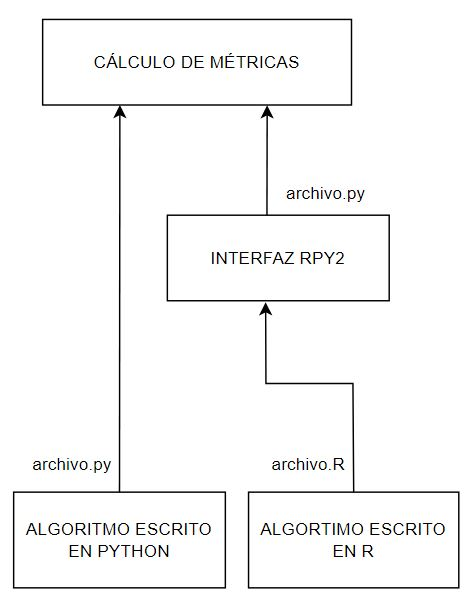
\includegraphics[width=3in]{estructura-interfaz-rpy2.jpg}
  \caption{Estructura del entorno de ejecución}
  \label{img:estructura del entorno de ejecucion}
\end{figure}

Determinadas las métricas dependientes del entorno de ejecución, los resultados diferirán según el medio 
en el que se realicen las pruebas. Se muestra en la tabla \ref{tab:caracteristicas del entorno de ejecucion} 
las características del entorno empleado.

\begin{table}[h]
  \begin{center}
    \begin{tabular}{| c | c | c |} \hline 
     \textbf{Procesador (CPU)} & \textbf{Memoria RAM} & \textbf{Tarjeta Gráfica (GPU)} \\ \hline
     AMD Ryzen 7 2700 Eight-Core 3.20 GHz & 16,0 GB & NVIDIA GeForce RTX 2060 SUPER \\ \hline
    \end{tabular}
    \caption{Características del entorno de ejecución}
    \label{tab:caracteristicas del entorno de ejecucion}
  \end{center}
\end{table} 

\textbf{Tiempo de ejecución:}

La primera de las mediciones tiene que ver con el tiempo en realizar el proceso completo de minado. En el 
momento en el que el algoritmo comienza a extraer información se activa el contador, y este para cuando 
finaliza el proceso.

Cabe destacar que el cálculo de dicho tiempo abarca el proceso de minado al completo, desde el acceso al
contenido, hasta la transformación del mismo.

\textbf{Uso de CPU(\%):}

El uso de CPU es la cantidad total cantidad de procesador que consume la tarea a realizar. Permite valores 
por encima del 100\%, lo que indica que el proceso se ejecuta en múltiples hilos en diferentes núcleos de 
la CPU. La máquina que realizó las pruebas tiene un total de ocho núcleos, por lo que el 800\% significaría
que todos los núcleos trabajan al máximo en el proceso.

Para el cálculo del uso de CPU se emplea la función \emph{cpu\_percent(interval)}, que devuelve un número 
que representa la utilización actual de la CPU en todo el sistema en forma de porcentaje. Cuando la variable 
\emph{interval} es mayor que cero, compara los tiempos de CPU del sistema transcurridos antes y después de 
dicho intervalo.

\textbf{Uso de de memoria física o RAM(\%):}

La memoria real también conocida como memoria física o RAM, es la tercera métrica registrada. Simplemente 
mide la cantidad de memoria física que el proceso está empleando. Como recordatorio, la máquina en la que 
se realiza la evaluación tiene un total de 16GB de memoria física.

Para el cálculo del uso de memoria RAM se emplea la función \emph{virtual\_memory()}, que devuelve 
estadísticas sobre el uso de la memoria física total.







































\chapter{Análisis y comparativa de paquetes}
\label{cha:analisis y comparativa de paquetes}

Tras la exposición de las diferentes variables y métricas que conformaran la evaluación, se realiza el
correspondiente análisis y comparación de paquetes. Inicialmente, el análisis será individual de cada 
paquete, para finalmente hacer una comparativa conjunta.

\section{Evaluación individual de paquetes}
\label{sec:evaluacion individual de paquetes}

A continuación se realiza un análisis individual de los resultados obtenidos de cada paquete. Adicionalmente, 
se incluyen resultados de otros paquetes con el objetivo de efectuar una pequeña comparación entre los 
mismos.

\section*{inscriptis}

El primer paquete sometido a análisis será \textbf{inscriptis}, el cual debemos instalar e importar en el
fragmento de código respectivo. En cuanto a su instalación, es muy sencilla, simplemente se debe ejecutar
la siguiente instrucción en la línea de comandos: \emph{\$ pip install inscriptis}.

\begin{codefloat}
    \inputencoding{latin1}
    \lstinputlisting[style=CppExample, showstringspaces=false]{scripts/script-inscriptis.py}
    \inputencoding{utf8}
    \caption{Función de ejecución de inscriptis}
    \label{cod:funcion de ejecucion de inscriptis}
\end{codefloat}

En cuanto al código mostrado en \ref{cod:funcion de ejecucion de inscriptis}, es muy simple. Se itera sobre 
los archivos HTML a analizar, y se emplea la función \emph{get\_text()} para obtener la información deseada. 
Dicha información se almacena posteriormente de forma ordenada sobre un diccionario.

Para conservar la información obtenida y no ejecutar el algoritmo múltiples veces, el diccionario obtenido
se almacena en un archivo \emph{json} propio del paquete. De esta forma, el archivo \emph{inscriptis.json} 
conserva todos los fragmentos de texto obtenidos del minado web anterior.

Una vez ejecutado el algoritmo, se realizan todos los cálculos pertinentes y se determinan las puntuaciones
obtenidas. En el caso de \textbf{inscriptis}, se muestran en la tabla
\ref{tab:tabla - resultados de la evaluacion de inscriptis} los resultados obtenidos.

\begin{table}[h]
    \begin{center}
      \begin{tabular}{| c | c | c | c | c | c | c | c |} \hline 
       \textbf{Nombre} & \textbf{Accuracy} & \textbf{Precision}  & \textbf{Recall} & \textbf{F1} & \textbf{RAM(\%)} & \textbf{CPU(\%)} & \textbf{Time Exec.(s)} \\ \hline
       inscriptis & 0.5414 & 0.5404 & 0.9875 & 0.6985 & 45.0 & 0.2 & 2.1005 \\ \hline
      \end{tabular}
      \caption{Tabla - Resultados de la evaluación de inscriptis}
      \label{tab:tabla - resultados de la evaluacion de inscriptis}
    \end{center}
\end{table} 

En forma de gráfica, se muestra en la figura \ref{img:grafica - resultados de la evaluacion de inscriptis}
los cálculos obtenidos en referencia a las métricas independientes del entorno de ejecución. Analizando
estas métricas, y sabiendo que \emph{f1} determina la calidad en general de la extracción, podemos concluir
que \textbf{inscriptis} realiza un equilibrado trabajo en el minado web.

\begin{figure}[tphb]
    \centering
    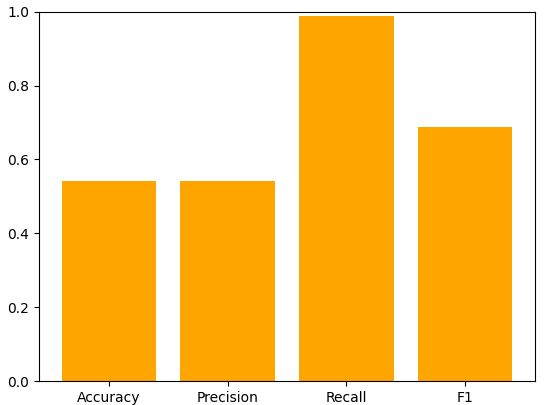
\includegraphics[width=5in]{resultados-inscriptis.jpg}
    \caption{Gráfica - Resultados de la evaluación de inscriptis}
    \label{img:grafica - resultados de la evaluacion de inscriptis}
\end{figure}

Por otro lado, respecto a las métricas dependientes del entorno, al solo tener una medición de referencia 
no podemos decir demasiado. El uso de memoria RAM parece elevado dadas las especificaciones del entorno. 
Por el contrario, el uso de CPU es mínimo. Algo sorprendente es que \textbf{inscriptis} haya sido capaz de 
analizar 101 documentos HTML en únicamente dos segundos.

\section*{Beautiful Soup}

El segundo paquete sometido a análisis será \textbf{Beautiful Soup}, el cual debemos instalar e importar 
en el fragmento de código respectivo. En cuanto a su instalación, es muy sencilla, simplemente se debe 
ejecutar la siguiente instrucción en la línea de comandos: \emph{\$ pip install beautifulsoup4}.

Como se observa en el fragmento de código \ref{cod:funcion de ejecucion beautiful soup}, la función es muy
similar a la vista con \textbf{inscriptis}. Se itera sobre los documentos HTML a analizar y se aplica la
función \emph{get\_text()} para extraer la información.

\begin{codefloat}
    \inputencoding{latin1}
    \lstinputlisting[style=CppExample, showstringspaces=false]{scripts/script-beautifulsoup.py}
    \inputencoding{utf8}
    \caption{Función de ejecución de Beautiful Soup}
    \label{cod:funcion de ejecucion beautiful soup}
\end{codefloat}

Debemos recordar que \textbf{Beautiful Soup} permite seleccionar entre varios tipos de analizadores, ya sea
\emph{html.parse}, \emph{lxml} o \emph{html5lib}. Tras la ejecución de \textbf{Beautiful Soup} empleando
\emph{html.parse} como analizador, se procede con el cálculo de métricas. Los resultados obtenidos se 
muestran en la tabla \ref{tab:tabla - resultados de la evaluacion de beautiful soup html.parse}.

\begin{table}[h]
    \begin{center}
      \begin{tabular}{| c | c | c | c | c | c | c | c |} \hline 
       \textbf{Nombre} & \textbf{Accuracy} & \textbf{Precision}  & \textbf{Recall} & \textbf{F1} & \textbf{RAM(\%)} & \textbf{CPU(\%)} & \textbf{Time Exec.(s)} \\ \hline
       Beau. Soup & 0.5165 & 0.5129 & 0.9928 & 0.6764 & 47.0 & 4.3 & 4.0882 \\ \hline
      \end{tabular}
      \caption{Tabla - Resultados de la evaluación de Beautiful Soup \emph{(html.parse)}}
      \label{tab:tabla - resultados de la evaluacion de beautiful soup html.parse}
    \end{center}
\end{table} 

Se emplea ahora \emph{lxml} como analizador estándar y se procede con el cálculo de métricas. Los resultados
obtenidos se muestran en la tabla \ref{tab:tabla - resultados de la evaluacion de beautiful soup lxml}.

\begin{table}[h]
    \begin{center}
      \begin{tabular}{| c | c | c | c | c | c | c | c |} \hline 
       \textbf{Nombre} & \textbf{Accuracy} & \textbf{Precision}  & \textbf{Recall} & \textbf{F1} & \textbf{RAM(\%)} & \textbf{CPU(\%)} & \textbf{Time Exec.(s)} \\ \hline
       Beau. Soup & 0.5165 & 0.5129 & 0.9928 & 0.6764 & 38.1 & 3.4 & 3.2183 \\ \hline
      \end{tabular}
      \caption{Tabla - Resultados de la evaluación de Beautiful Soup \emph{(lxml)}}
      \label{tab:tabla - resultados de la evaluacion de beautiful soup lxml}
    \end{center}
\end{table}

Se emplea ahora \emph{html5lib} como analizador estándar y se procede con el cálculo de métricas. Los 
resultados obtenidos se muestran en la tabla 
\ref{tab:tabla - resultados de la evaluacion de beautiful soup html5lib}.

\begin{table}[h]
    \begin{center}
      \begin{tabular}{| c | c | c | c | c | c | c | c |} \hline 
       \textbf{Nombre} & \textbf{Accuracy} & \textbf{Precision}  & \textbf{Recall} & \textbf{F1} & \textbf{RAM(\%)} & \textbf{CPU(\%)} & \textbf{Time Exec.(s)} \\ \hline
       Beau. Soup & 0.1327 & 0.1315 & 0.9921 & 0.2323 & 39.1 & 3.4 & 9.8604 \\ \hline
      \end{tabular}
      \caption{Tabla - Resultados de la evaluación de Beautiful Soup \emph{(html5lib)}}
      \label{tab:tabla - resultados de la evaluacion de beautiful soup html5lib}
    \end{center}
\end{table}

En forma de gráfica, se muestra en \ref{img:grafica - resultados de la evaluacion de beautiful soup} los 
cálculos obtenidos en referencia a las métricas independientes del entorno de ejecución. Realizando un
análisis, podemos determinar que el uso de \emph{html.parse} o \emph{lxml} no altera la calidad de la 
información obtenida. Por el contrario cuando se emplea \emph{html5lib} tanto la cantidad de predicciones 
correctas, como la exclusión de contenido \emph{boilerplate} se reduce drásticamente.

\begin{figure}[tphb]
    \centering
    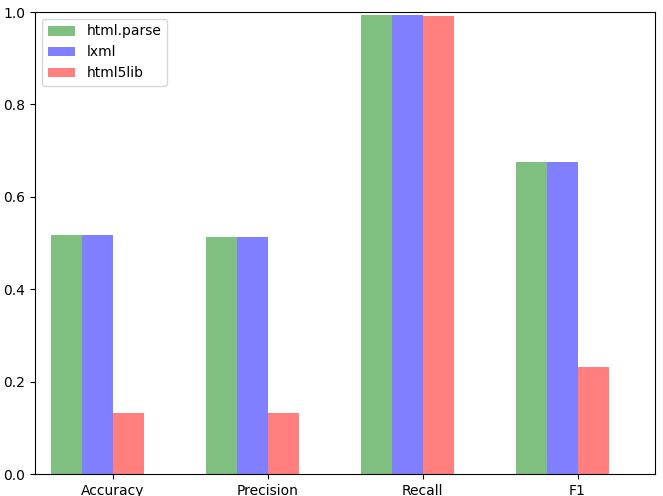
\includegraphics[width=4.6in]{resultados-beautifulsoup.jpg}
    \caption{Gráfica - Resultados de la evaluación de Beautiful Soup}
    \label{img:grafica - resultados de la evaluacion de beautiful soup}
\end{figure}

Por otro lado, respecto a las métricas dependientes del entorno, el uso de memoria RAM, al igual que el uso
de CPU, es similar en todos los analizadores. Véase \ref{img:grafica - resultados de la evaluacion de beautiful soup 2}.

\begin{figure}[tphb]
    \centering
    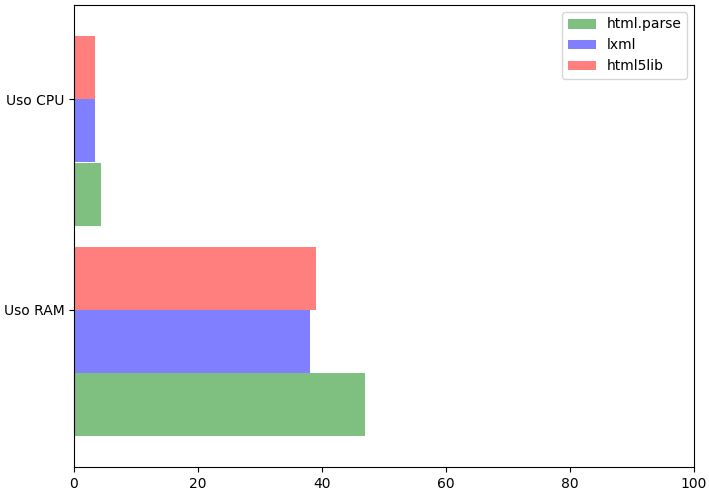
\includegraphics[width=4.6in]{resultados-beautifulsoup2.jpg}
    \caption{Gráfica - Resultados de la evaluación de Beautiful Soup 2}
    \label{img:grafica - resultados de la evaluacion de beautiful soup 2}
\end{figure}

\section*{jusText}

El siguiente paquete sometido a análisis será \textbf{jusText}, el cual debemos instalar e importar en el
fragmento de código respectivo. En cuanto a su instalación, es muy sencilla, simplemente se debe ejecutar
la siguiente instrucción en la línea de comandos: \emph{\$ pip install justext}.

Como se observa en el fragmento de código \ref{cod:funcion de ejecucion de jusText}, la forma en la que
se extrae texto de documentos HTML es muy similar a las vistas anteriormente. La principal diferencia es
que en este caso \textbf{jusText}, previamente a la extracción, realiza las siguientes acciones:

\begin{itemize}
    \item Clasificación de bloques.
    \item Preprocesamiento de bloques de cabecera.
    \item Reclasificación de bloques.
    \item Postprocesamiento de bloques de cabecera.
\end{itemize}

\begin{codefloat}
    \inputencoding{latin1}
    \lstinputlisting[style=CppExample, showstringspaces=false]{scripts/script-justext.py}
    \inputencoding{utf8}
    \caption{Función de ejecución de jusText}
    \label{cod:funcion de ejecucion de jusText}
\end{codefloat}

Como el resto de algoritmos, para conservar la información obtenida y no ejecutar el código múltiples 
veces, el diccionario obtenido se almacena en un archivo \emph{json} propio del paquete. De esta forma, 
el \emph{justext.json} conserva todos los fragmentos de texto obtenidos del minado web anterior.

Una vez ejecutado el algoritmo, se realizan todos los cálculos pertinentes y se determinan las puntuaciones 
obtenidas. En el caso de \textbf{jusText}, los resultados obtenidos se muestran en la tabla 
\ref{tab:tabla - resultados de la evaluacion de justext}.

\begin{table}[h]
    \begin{center}
      \begin{tabular}{| c | c | c | c | c | c | c | c |} \hline 
       \textbf{Nombre} & \textbf{Accuracy} & \textbf{Precision}  & \textbf{Recall} & \textbf{F1} & \textbf{RAM(\%)} & \textbf{CPU(\%)} & \textbf{Time Exec.(s)} \\ \hline
       jusText & 0.7668 & 0.8649 & 0.8573 & 0.8610 & 45.1 & 0.5 & 2.9546 \\ \hline
      \end{tabular}
      \caption{Tabla - Resultados de la evaluación de jusText}
      \label{tab:tabla - resultados de la evaluacion de justext}
    \end{center}
\end{table}

En forma de gráfica, se muestra en la figura \ref{img:grafica - resultados de la evaluacion de justext}
los cálculos obtenidos en referencia a las métricas independientes del entorno de ejecución. Con un simple
vistazo, es posible determinar que el algoritmo de \textbf{jusText} realiza un buen trabajo en al selección
de contenido relevante. 

\begin{figure}[tphb]
    \centering
    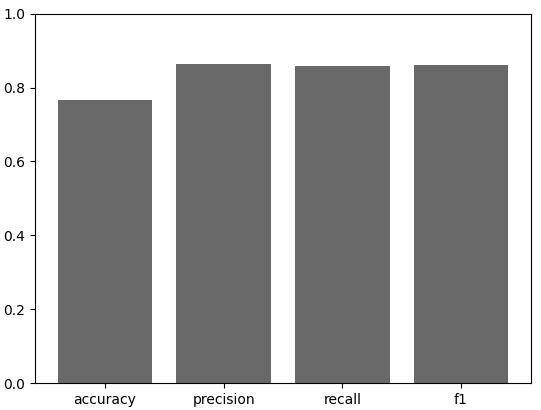
\includegraphics[width=5in]{resultados-justext.jpg}
    \caption{Gráfica - Resultados de la evaluación de jusText}
    \label{img:grafica - resultados de la evaluacion de justext}
\end{figure}

Por otro lado, con respecto a las métricas dependientes del entorno de ejecución, se debe remarcar que
\textbf{jusText} es un paquete de minado web muy bien optimizado. A pesar de realizar todo el trabajo previo
a la extracción, mantiene un buen tiempo de ejecución y escaso uso de la CPU.

\section*{html\_text}

El siguiente paquete sometido a análisis será \textbf{html\_text}, el cual debemos instalar e importar en 
el fragmento de código respectivo. En cuanto a su instalación, simplemente se debe ejecutar la siguiente 
instrucción en la línea de comandos: \emph{\$ pip install html-text}.

\begin{codefloat}
    \inputencoding{latin1}
    \lstinputlisting[style=CppExample, showstringspaces=false]{scripts/script-htmltext.py}
    \inputencoding{utf8}
    \caption{Función de ejecución de html\_text}
    \label{cod:funcion de ejecucion de htmltext}
\end{codefloat}

En el fragmento de código \ref{cod:funcion de ejecucion de htmltext} se muestra como \textbf{html\_text} 
extrae texto de los diferentes documentos HTML. La función \emph{extract\_text()} emplea expresiones 
\emph{xPath} y normalizaciones de espacio para obtener una mejor calidad en los resultados.

Una vez ejecutado el algoritmo, se realizan todos los cálculos pertinentes y se determinan las puntuaciones 
obtenidas. En el caso de \textbf{html\_text}, los resultados obtenidos se muestran en la tabla 
\ref{tab:tabla - resultados de la evaluacion de htmltext}.

\begin{table}[h]
    \begin{center}
      \begin{tabular}{| c | c | c | c | c | c | c | c |} \hline 
       \textbf{Nombre} & \textbf{Accuracy} & \textbf{Precision}  & \textbf{Recall} & \textbf{F1} & \textbf{RAM(\%)} & \textbf{CPU(\%)} & \textbf{Time Exec.(s)} \\ \hline
       html\_text & 0.5166 & 0.513 & 0.9928 & 0.6765 & 44.9 & 0.5 & 1.1800 \\ \hline
      \end{tabular}
      \caption{Tabla - Resultados de la evaluación de html\_text}
      \label{tab:tabla - resultados de la evaluacion de htmltext}
    \end{center}
\end{table}

Tanto en la tabla \ref{tab:tabla - resultados de la evaluacion de htmltext} como en su correspondiente
gráfica \ref{img:grafica - resultados de la evaluacion de htmltext}, podemos observar que el algoritmo
cumple asequiblemente con unos requisitos mínimos con respecto a aquellas métricas no dependientes del
entorno de ejecución.

\begin{figure}[tphb]
    \centering
    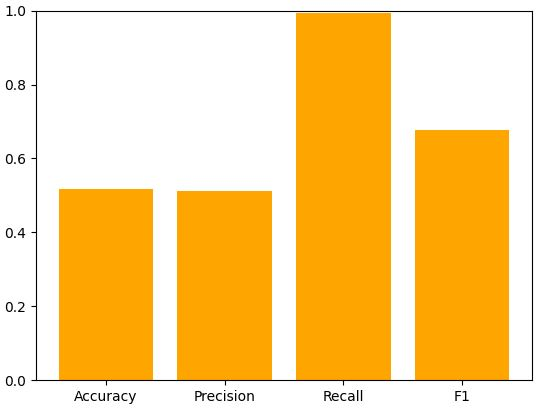
\includegraphics[width=5in]{resultados-htmltext.jpg}
    \caption{Gráfica - Resultados de la evaluación de html\_text}
    \label{img:grafica - resultados de la evaluacion de htmltext}
\end{figure}

En cuanto a las métricas dependientes de entorno, es cierto que el algoritmo emplea pocos recursos, y su
tiempo de ejecución es reducido. Esto se debe a que su heurística es simple, el uso único de expresiones
\emph{xPath} optimiza los recursos. ¿Compensa sobre la calidad de la extracción? Lo veremos en al siguiente
sección, cuando comparemos la \emph{performance} de todos los paquetes.

\section*{html2text}

El siguiente paquete sometido a análisis será \textbf{html2text}, el cual debemos instalar e importar en 
el fragmento de código respectivo. En cuanto a su instalación, simplemente se debe ejecutar la siguiente 
instrucción en la línea de comandos: \emph{\$ pip install html2text}.

\begin{codefloat}
    \inputencoding{latin1}
    \lstinputlisting[style=CppExample, showstringspaces=false]{scripts/script-html2text.py}
    \inputencoding{utf8}
    \caption{Función de ejecución de html2text}
    \label{cod:funcion de ejecucion de html2text}
\end{codefloat}

En el fragmento de código \ref{cod:funcion de ejecucion de html2text} se muestra como \textbf{html2text}
extrae texto de los diferentes documentos HTML. Si recordamos, \textbf{html2text} no se caracteriza por
disponer de una heurística compleja, el algoritmo simplemente hace uso de \emph{html.parse} para analizar
el documento y envolver todos los párrafos del texto proporcionado.

\begin{table}[h]
    \begin{center}
      \begin{tabular}{| c | c | c | c | c | c | c | c |} \hline 
       \textbf{Nombre} & \textbf{Accuracy} & \textbf{Precision}  & \textbf{Recall} & \textbf{F1} & \textbf{RAM(\%)} & \textbf{CPU(\%)} & \textbf{Time Exec.(s)} \\ \hline
       html2text & 0.5105 & 0.5107 & 0.9804 & 0.6715 & 44.6 & 1.8 & 4.4020 \\ \hline
      \end{tabular}
      \caption{Tabla - Resultados de la evaluación de html2text}
      \label{tab:tabla - resultados de la evaluacion de html2text}
    \end{center}
\end{table}

Los resultados mostrados, tanto en la tabla \ref{tab:tabla - resultados de la evaluacion de html2text} como
en la gráfica \ref{img:grafica - resultados de la evaluacion de html2text}, hacen reflejo de la simplicidad
de su heurística. A pesar de todo ello, la calidad en general de la extracción no está muy lejos de la media.

\begin{figure}[tphb]
    \centering
    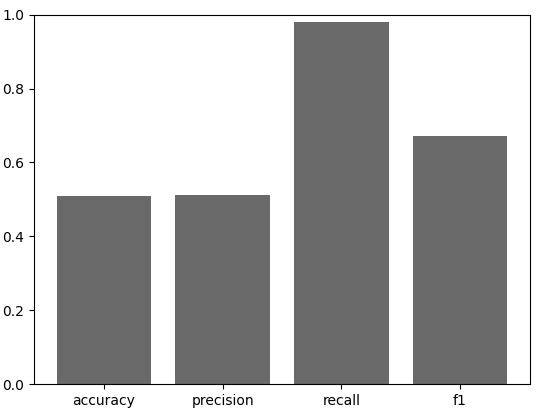
\includegraphics[width=4.7in]{resultados-html2text.jpg}
    \caption{Gráfica - Resultados de la evaluación de html2text}
    \label{img:grafica - resultados de la evaluacion de html2text}
\end{figure}

\section*{Readability}






% Optional in PFCs
%
\chapter{Pliego de condiciones}
\label{cha:pliego-de-condiciones}

Blah, blah, blah.

%%% Local Variables:
%%% TeX-master: "../book"
%%% End:


%Obligatorio en TFGs
\chapter{Conclusiones y futuras líneas de trabajo}
\label{cha:conclusiones y futuras lineas de trabajo}

%
% Fin de la seccion de capitulos
%%%%%%%%%%%%%%%%%%%%%%%%%%%%%%%%%%%%%%%%%%%%%%%%%%%%%%%%%%%%%%%%%%%%%%%%%%%
%%%%%%%%%%%%%%%%%%%%%%%%%%%%%%%%%%%%%%%%%%%%%%%%%%%%%%%%%%%%%%%%%%%%%%%%%%%

%%%%%%%%%%%%%%%%%%%%%%%%%%%%%%%%%%%%%%%%%%%%%%%%%%%%%%%%%%%%%%%%%%%%%%%%%%%
%
% Generic template for TFC/TFM/TFG/Tesis
%
% $Id: bibliography.tex,v 1.9 2015/06/05 00:10:32 macias Exp $
%
% By:
%  + Javier Macías-Guarasa. 
%    Departamento de Electrónica
%    Universidad de Alcalá
%  + Roberto Barra-Chicote. 
%    Departamento de Ingeniería Electrónica
%    Universidad Politécnica de Madrid   
% 
% Based on original sources by Roberto Barra, Manuel Ocaña, Jesús Nuevo,
% Pedro Revenga, Fernando Herranz and Noelia Hernández. Thanks a lot to
% all of them, and to the many anonymous contributors found (thanks to
% google) that provided help in setting all this up.
%
% See also the additionalContributors.txt file to check the name of
% additional contributors to this work.
%
% If you think you can add pieces of relevant/useful examples,
% improvements, please contact us at (macias@depeca.uah.es)
%
% You can freely use this template and please contribute with
% comments or suggestions!!!
%
%%%%%%%%%%%%%%%%%%%%%%%%%%%%%%%%%%%%%%%%%%%%%%%%%%%%%%%%%%%%%%%%%%%%%%%%%%%

%\bibliographystyle{plainnat}
%\bibliographystyle{dinat}
%\bibliographystyle{unsrt}
\bibliographystyle{IEEEtran}

% The following is overly complicated because I was not able to do so in
% another way. The problem is the bibliography command being "called"
% from both the root and anteproyecto directories...
%
% Here define as many bibfiles as needed
\newcommand{\mybibfileOne}{biblio/biblio.bib}
%\newcommand{\mybibfileTwo}{biblio/biblio2.bib}
%...
%\newcommand{\mybibfileN}{biblio/biblioN}

% This is for a single bib file
\newcommand{\mybibfiles}{\myreferencespath\mybibfileOne}
% but do this for multiple files
%\newcommand{\mybibfiles}{\myreferencespath\mybibfile1,\myreferencespath\mybibfile2,...,\myreferencespath\mybibfileN}

% Do not touch this
\inputencoding{latin1}
\bibliography{\mybibfiles}
\inputencoding{utf8}

%%% Local Variables:
%%% TeX-master: "../book"
%%% coding: utf-8
%%% End:


 % Bibliografia

%%%%%%%%%%%%%%%%%%%%%%%%%%%%%%%%%%%%%%%%%%%%%%%%%%%%%%%%%%%%%%%%%%%%%%%%%%%
% Comienzo de apendices
%                                 

\begin{appendices}
  \chapter{Funcionamiento básico de un web scraper}
\label{cha:funcionamiento basico de un web scraper}

Siguiendo las directrices determinadas en la sección \ref{subsec:extraccion de los datos}, se
muestra el funcionamiento de un web scraper durante las tres fases definidas. Para ello se realizará un
pequeño ejemplo mostrando el comportamiento del mismo y de como interactúa con el servidor web al que
se desea acceder.

Para el desarrollo de este ejemplo se han empleado bibliotecas software basadas en el lenguaje de
programación R, capaces de extraer datos de cualquier web. En este caso la web sujeta al análisis será,
\emph{imdb} encargada de asignar un ranking entre películas y series.

\section{Fase de búsqueda}
\label{sec:fase de busqueda}

Antes de comenzar con la primera de las tres etapas, debemos asegurarnos que nuestro agente software
cumple con todos los aspectos ético-legales descritos en la sección \ref{sec:aspectos etico-legales del web
scraping}. Los términos y servicios de la página deberán ser leídos, al igual que el documento
\emph{'robots.txt'} con el objetivo de conocer cuáles son los accesos disponibles y el índice de solicitudes
a realizar.

En el fragmento de código \ref{cod:solicitud del documento robots.txt} se muestra la solicitud al servidor
realizada. A través de la biblioteca \emph{robotstxt} \cite{robotstxt-cran} y haciendo uso de la función
\emph{get\_robotstxt} se obtiene el documento deseado.

Es posible que la solicitud del documento no se realice correctamente, pues o bien la página no dispone
del documento en ese instante, o la función ha fallado durante su solicitud. En cualquiera de estos dos
escenarios, es posible realizar una doble comprobación accediendo al mismo a través de la propia URL,
\emph{https://www.imdb.com/robots.txt}.

\begin{codefloat}
\inputencoding{latin1}
\lstinputlisting[style=CppExample]{scripts/ejemplo-basico-web-scraping-1.R}
\inputencoding{utf8}
\caption{Solicitud del documento \emph{robots.txt}}
\label{cod:solicitud del documento robots.txt}
\end{codefloat}

\begin{Schunk}
    \begin{Soutput}
    # robots.txt for https://www.imdb.com properties
    User-agent: *
    Disallow: /OnThisDay
    Disallow: /ads/
    Disallow: /ap/
    Disallow: /mymovies/
    Disallow: /r/
    Disallow: /register
    Disallow: /registration/
    ...
    \end{Soutput}
\end{Schunk}
    

Una vez se ha accedido al documento \emph{'robots.txt'}, conociendo los posibles accesos al servidor, y
determinando el número de solicitudes máximas por segundo, es posible acceder y descargar el fichero
HTML de forma segura. Para este propósito se empleará la función \emph{read\_html} de la biblioteca
\emph{xml2} \cite{xml2-cran} la cual se detalla a continuación.

\begin{codefloat}
\inputencoding{latin1}
\lstinputlisting[style=CppExample]{scripts/ejemplo-basico-web-scraping-2.R}
\inputencoding{utf8}
\caption{Acceso y descarga del archivo HTML}
\label{cod:acceso y descarga del archivo html}
\end{codefloat}

El valor que retorna la función \emph{read\_html}, se trata del archivo HTML integro, donde se incluyen
cabecera, cuerpo y demás etiquetas del mismo. Una vez que se dispone de la página, es posible comenzar
con la extracción de datos de interés de la misma.

\section{Fase de extracción}
\label{sec:fase de extraccion}

Para el minado se empleará \emph{rvest} \cite{rvest-cran}, una de las bibliotecas software más comunes en
este aspecto, diseñada para trabajar con \emph{magrittr} \cite{magrittr-cran} y facilitar tareas de la
extracción. Además, será necesario el uso de funciones como \emph{html\_nodes()} y \emph{html\_text()}.

Durante esta fase de extracción se obtendrán tanto los títulos como el ranking asignado a cada película o
serie. Para realizar la extracción de forma correcta, se deberá conocer la etiqueta HTML que envuelve dicha
información.

\begin{codefloat}
\inputencoding{latin1}
\lstinputlisting[style=CppExample]{scripts/ejemplo-basico-web-scraping-3.R}
\inputencoding{utf8}
\caption{Extracción de datos de interés del documento}
\label{cod:extraccion de datos de interes del documento}
\end{codefloat}

\begin{Schunk}
    \begin{Soutput}
    [1] "1." "2." "3." "4." "5." "6."
    
    [1] "Animales nocturnos"   "Train to Busan"       "La llegada (Arrival)"
    [4] "Escuadrón suicida"    "Deadpool"             "Hush (Silencio)"     
    \end{Soutput}
\end{Schunk}
    

\section{Fase de transformación}
\label{sec:fase de transformacion}

Una vez los datos han sido extraídos, la última fase consiste en la transformación de los mismos. Los datos
desordenados deberán ser convertidos en estructuras de datos ordenadas y coherentes con el fin su posible
almacenamiento en una base de datos.

\begin{codefloat}
\inputencoding{latin1}
\lstinputlisting[style=CppExample]{scripts/ejemplo-basico-web-scraping-4.R}
\inputencoding{utf8}
\caption{Transformación de datos en un data frame}
\label{cod:transformacion de datos en un data frame}
\end{codefloat}

\begin{Schunk}
    \begin{Soutput}
      Rank                Title
    1   1.   Animales nocturnos
    2   2.       Train to Busan
    3   3. La llegada (Arrival)
    4   4.    Escuadrón suicida
    5   5.             Deadpool
    6   6.      Hush (Silencio)
    \end{Soutput}
\end{Schunk}

Una vez los datos han sido ordenados en una estructura de datos propia, en este caso un data frame, es
posible trabajar con ellos de forma más cómoda y sencilla.








  \chapter{Analizadores empleados en los paquetes de web scraping}
\label{cha:analizadores empleados en los paquetes de web scraping}

Este apéndice tiene como objetivo introducir aquellos aspectos más relevantes relacionados con los
analizadores, también conocidos como \emph{parsers}, empleados en el web scraping. A lo largo de esta 
sección se realizará una pequeña sinopsis de aquellas herramientas empleadas en los algoritmos de extracción 
de los paquetes definidos en la sección \ref{sec:bibliotecas de python encontradas durante el proceso de 
busqueda}.

A modo de introducción cabe destacar que un analizador sintáctico, es un programa informático que analiza
una cadena de símbolos según las reglas de una gramática formal \cite{parser-lexer}. Generalmente, los 
analizadores se componen de dos partes, por un lado, un analizador sintáctico, y por otro un analizador 
léxico. Mientras que el analizador léxico crea tokens a partir de una secuencia de caracteres de entrada, 
el analizador sintáctico convierte los tokens en otras estructuras.

\begin{figure}[tphb]
    \centering
    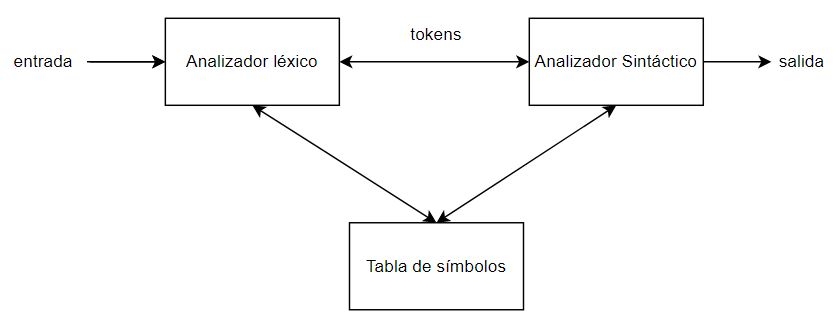
\includegraphics[width=5.5in]{parser-structure.jpg}
    \caption{Estructura basica de un analizador}
    \label{img:estructura basica de un analizador}
\end{figure}

\section{lxml}
\label{sec:lxml}

Uno de los analizadores más comunes en todos los algoritmos de minado web es \textbf{lxml} \cite{lxml}. 
Esta biblioteca de Python permite procesar tanto documentos XML como HTML.

Como la gran mayoría de analizadores, \textbf{lxml} convierte el texto de entrada en una estructura tipo 
árbol. Esto permite navegar por la propia estructura en busca de la información que se desea de forma 
sencilla. 

En el caso del web scraping, la manera en la que \textbf{lxml} es capaz de encontrar información valiosa, 
es decir texto, es a través de expresiones \emph{XPath}. Se muestra un pequeño ejemplo a continuación.

\begin{Schunk}
    \begin{Soutput}
        > html.xpath("string()")
        # TEXTTAIL

        > html.xpath("//text()")
        # ['TEXT', 'TAIL']
    \end{Soutput}
\end{Schunk}

Cabe destacar que el resultado dado por una expresión \emph{XPath} es un objeto especial que conoce parte de su
estructura. Esto permite ejecutar operaciones sobre este elemento y saber de dónde proviene a través de
diferentes métodos.

\subsection{lxml.html}
\label{subsec:lxml.html}

¿Qué ocurre con los documentos HTML mal formados? Para este propósito, se creó lo que se conoce como
\textbf{lxml.html} \cite{lxml}. Un paquete de Python especial para tratar con documentos HTML, el cual 
a diferencia del analizador base, proporciona una API de elementos propia de HTML, así como una serie de 
utilidades para tareas comunes de procesamiento de los mismos.

\begin{Schunk}
    \begin{Soutput}
        > broken_html = "<html><head><body><h1>page title</h3>"
        > parser = etree.HTMLParser()
        > tree   = etree.parse(StringIO(broken_html), parser)
        > result = etree.tostring(tree.getroot(), method="html")
        # <html><head></head><body><h1>page title</h1></body></html>
    \end{Soutput}
\end{Schunk}

Como se puede observar, incluso analizando documentos realmente mal formados, el analizador es capaz de
crear una estructura propia de un documento HTML. A partir de ahí, es posible aplicar expresiones 
\emph{XPath} con el fin de recorrer el árbol generado y recuperar información de valor.

\subsection{soupparser}
\label{subsec:soupparser}

Otro de los analizadores propios de \textbf{lxml} es \textbf{soupparser} \cite{lxml} propio del paquete
\textbf{Beautiful Soup}. La forma en la que \textbf{lxml} interactúa con \textbf{Beautiful Soup}, es a 
través del módulo \textbf{lxml.html.soupparser} el cual proporciona una seria de funciones principales. 

Por un lado, tanto \emph{fromstring()} como \emph{parse()} se emplean para analizar ya sea una cadena o un 
archivo HTML, por otro lado \emph{convert\_tree()} se emplea para convertir un árbol \textbf{Beautiful Soup} 
existente en una lista de elementos de nivel superior.

\begin{Schunk}
    \begin{Soutput}
        > tag_soup = '''<meta/><head></head><body>Hi all<p>'''
        > root = fromstring(tag_soup)
        # <html><meta/><head></head><body>Hi all<p/></body></html>
    \end{Soutput}
\end{Schunk}

Imaginemos que se dispone de una cadena HTML mal formada como la mostrada en el ejemplo. Al ser una cadena,
se emplea \emph{fromstring()} para realizar un análisis de la misma. Como vemos la salida también puede
provocar algún error, puesto que no es exactamente una estructura propia de HTML.

\section{html5lib}
\label{sec:html5lib}

\textbf{html5lib} \cite{html5lib} es un paquete de Python que implementa el algoritmo de análisis sintáctico 
de HTML5. Proporciona una interfaz similar a la del módulo \textbf{lxml.html} \ref{subsec:lxml.html} con 
métodos como \emph{fromstring()} o \emph{parse()} que operan de la misma manera que las funciones de análisis 
de HTML normales.

Al igual que \textbf{lxml.html}, este paquete también trabaja con árboles de objetos, pero en este caso 
normaliza algunos elementos y estructuras a un formato común. Por ejemplo, incluso si una tabla no tiene 
una etiqueta del tipo \emph{<tbody>}, se inyectará una automáticamente.

\begin{Schunk}
    \begin{Soutput}
        > tostring(html5parser.fromstring("<table><td>foo"))
        # '<table><tbody><tr><td>foo</td></tr></tbody></table>'
    \end{Soutput}
\end{Schunk}

\section{html.parser}
\label{sec:html.parser}

\textbf{html.parser} \cite{html-parser} es un módulo de Python que define una clase HTMLParse como base 
para analizar archivos HTML y XHTML. Este módulo trabaja alrededor de etiquetas, pues llama a métodos de 
manejo cuando se encuentran etiquetas de inicio, etiquetas finales, texto, comentarios y otros elementos 
de marcado.

\begin{Schunk}
    \begin{Soutput}
        > parser.feed('<p><a class=link href=#main>tag soup</p ></a>')
        # Start tag: p
        # Start tag: a
        # Data     : tag soup
        # End tag  : p
        # End tag  : a
    \end{Soutput}
\end{Schunk}

Como se puede observar, el algoritmo es capaz de detectar etiquetas tanto de apertura, como de cierre incluso
en documentos HTML mal formados como este. Esto hace que la búsqueda de información valiosa, en este caso
texto, sea sencilla.

\section{XML}
\label{sec:xml}

\textbf{XML} \cite{xml-cran} es un paquete de R que se encarga de realizar el análisis de documentos XML
y HTML. Además del proceso de análisis, también proporciona acceso a un intérprete de \emph{XPath} que 
permite consultar nodos concretos de los documentos. Como contrapartida, no permite el uso de selectores 
CSS para examinar XML o HTML analizados.

Adicionalmente, hay que destacar que tiene algunos problemas de liberación de memoria que no puede resolver
adecuadamente el recolector de basura de R. Por ello, se han ido creando diferentes soluciones que abordan
este problema.

En cuanto al método de análisis, se recorre el árbol buscando la información que desee y se coloca en 
diferentes formas. Hay dos maneras de hacer esta iteración. Una es "recorrer" recursivamente el árbol 
empezando por el nodo raíz y procesándolo, la otra consiste procesar cada nodo hijo de la misma manera, 
trabajando en su nombre y atributos y luego en sus hijos, y así sucesivamente.


\section{xml2}
\label{sec:xml2}

Otro paquete de R que permite trabajar con ficheros XML y HTML es \textbf{xml2} \cite{xml2-cran}. Está
basado sobre la biblioteca \textbf{libxml2}. El paquete sigue los mismos objetivos que \textbf{XML}, por
lo que el análisis de ficheros compone la parte principal del mismo.

\textbf{xml2} tiene una jerarquía de clases muy sencilla que permite no preocuparse por el tipo de objeto
se está gestionando. Estas clases son clave y se definen a continuación:

\begin{enumerate}
    \item xml\_node: un solo nodo de un documento.
    \item xml\_doc: el documento completo. Actuar sobre un documento suele ser lo mismo que actuar sobre 
    el nodo raíz del documento.
    \item xml\_nodeset: un conjunto de nodos dentro del documento. Las operaciones sobre \emph{xml\_nodesets}
    se vectorizan, aplicando la operación sobre cada nodo del conjunto.
\end{enumerate}

A diferencia del paquete \textbf{XML}, \textbf{xml2} cuida la gestión de la memoria de forma transparente,
liberando aquella que haya sido utilizada por un documento tan pronto como se pierden todas las referencias
que apuntan a él. Además, la jerarquía de clases es más simple, por lo que no es necesario pensar
exactamente qué tipo de objeto se tiene, \textbf{xml2} simplemente hará lo correcto.




  \chapter{Métricas descartadas del proceso de evaluación}
\label{cha:metricas descartadas del proceso de evaluacion}

A lo largo del capítulo \ref{cha:seleccion de variables de analisis y proceso de estudio} se han definido
diferentes métricas capaces de comparar algoritmos de minado web. En este apéndice se definen aquellos
parámetros no incluidos en el clasificador. En la figura \ref{img:jerarquia de metricas descartadas} se 
muestra la relación entre variables y métricas. Se destacan, aquellas que han sido descartadas del proceso 
de evaluación.

\begin{figure}[tphb]
    \centering
    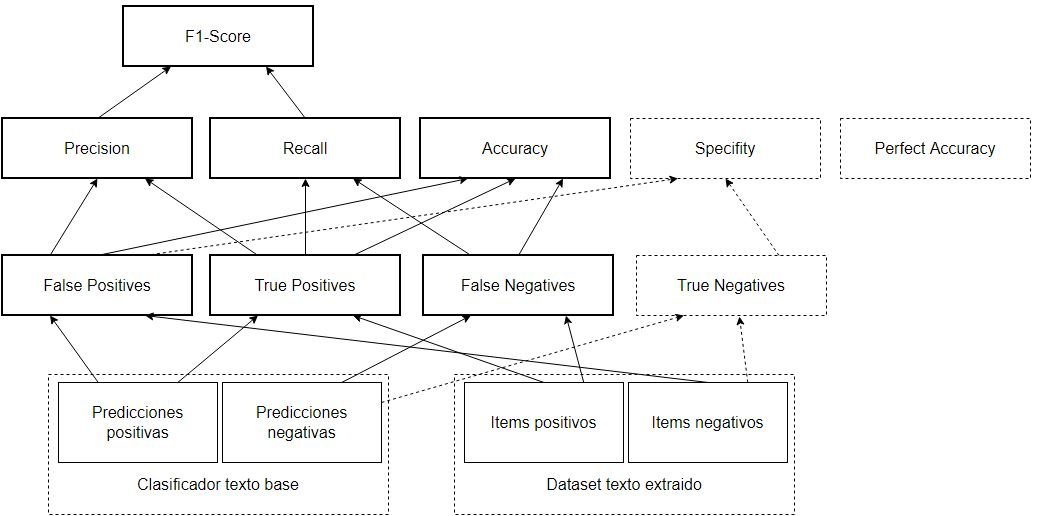
\includegraphics[width=7in]{estructura-metricas2.jpg}
    \caption{Jerarquía de métricas descartadas}
    \label{img:jerarquia de metricas descartadas}
\end{figure}

\section{\emph{Perfect accuracy}}
\label{sec:perfect accuracy}

Ya es sabido que la métrica \emph{accuracy}, mide la proporción de predicciones correctas sobre el número
total de predicciones, véase \ref{cod:calculo de la metrica accuracy}. Durante la búsqueda de una
característica que calculase este número, se pensó en una idea feliz en la que se comparaba
burdamente los tokens de los diferentes fragmentos de texto.

Esta métrica es fácil de entender pero bastante ruidosa, ya que una pequeña diferencia hace que toda la
página sea un fracaso. Veamos un pequeño fragmento de código, para comprobar la forma en la que se podría
incluir en nuestra evaluación.

\begin{codefloat}
    \inputencoding{latin1}
    \lstinputlisting[style=CppExample, showstringspaces=false]{scripts/evaluacion-perfect-accuracy.py}
    \inputencoding{utf8}
    \caption{Cálculo de la métrica \emph{perfect accuracy}}
    \label{cod:calculo de la metrica perfect accuracy}
\end{codefloat}

Se observa que la función convierte en tokens los fragmentos de texto correspondientes, para más tarde 
realizar la comparación pertinente. Este cálculo es muy similar al ya explicado en la sección 
\ref{subsubsec:comparacion de textos empleando el metodo palabra por deteccion}, donde se  comparaban 
textos a partir de los tokens de los mismos.

\section{\emph{Specificity}}
\label{sec:specificity}

La métrica conocida como \emph{Specificity} mide la cantidad de predicciones negativas realizadas que son
correctas. En otras palabras, mide como de mal a efectuado el minado web dicho algoritmo. La fórmula para
su cálculo es:

\begin{equation*}
    Specificity = \frac{True\;Negatives}{True\;Negatives + False\;Positives} = 
    \frac{N.\;of\;Correctly\;Predicted\;Negative\;Instances}{N.\;of\;Total\;Negative\;Instances\;in\;the\;Dataset}
\end{equation*}

Como se puede observar en el fragmento de código \ref{cod:calculo de la metrica specificity}, es necesario
contemplar los verdaderos negativos como nueva variable. Los verdaderos negativos se producen cuando el 
clasificador ha predicho un resultado negativo, y el resultado real fue negativo.

\begin{codefloat}
    \inputencoding{latin1}
    \lstinputlisting[style=CppExample, showstringspaces=false]{scripts/evaluacion-specificity.py}
    \inputencoding{utf8}
    \caption{Cálculo de la métrica \emph{specificity}}
    \label{cod:calculo de la metrica specificity}
\end{codefloat}
\end{appendices}

%
% Fin de apendices
%%%%%%%%%%%%%%%%%%%%%%%%%%%%%%%%%%%%%%%%%%%%%%%%%%%%%%%%%%%%%%%%%%%%%%%%%%%

\backmatter

%%%%%%%%%%%%%%%%%%%%%%%%%%%%%%%%%%%%%%%%%%%%%%%%%%%%%%%%%%%%%%%%%%%%%%%%%%%
%
% Generic template for TFC/TFM/TFG/Tesis
%
% $Id: backpage.tex,v 1.6 2018/12/12 15:29:21 macias Exp $
%
% By:
%  + Javier Macías-Guarasa. 
%    Departamento de Electrónica
%    Universidad de Alcalá
%  + Roberto Barra-Chicote. 
%    Departamento de Ingeniería Electrónica
%    Universidad Politécnica de Madrid   
% 
% Based on original sources by Roberto Barra, Manuel Ocaña, Jesús Nuevo,
% Pedro Revenga, Fernando Herránz and Noelia Hernández. Thanks a lot to
% all of them, and to the many anonymous contributors found (thanks to
% google) that provided help in setting all this up.
%
% See also the additionalContributors.txt file to check the name of
% additional contributors to this work.
%
% If you think you can add pieces of relevant/useful examples,
% improvements, please contact us at (macias@depeca.uah.es)
%
% You can freely use this template and please contribute with
% comments or suggestions!!!
%
%%%%%%%%%%%%%%%%%%%%%%%%%%%%%%%%%%%%%%%%%%%%%%%%%%%%%%%%%%%%%%%%%%%%%%%%%%%

%%%%%%%%%%%%%%%%%%%%%%%%%%%%%%%%%%%%%%%%%%%%%%%%%%%%%%%%%%%%%%%%%%%%%%%%%%%
% Right now (november 2013), it's only defined for TFGs at UAH
%%%%%%%%%%%%%%%%%%%%%%%%%%%%%%%%%%%%%%%%%%%%%%%%%%%%%%%%%%%%%%%%%%%%%%%%%%%

\ifthenelse{\equal{\mybookworktype}{TFG}}
{
  %%%%%%%%%%%%%%%%%%%%%%%%%%%%%%%%%%%%%%%%%%%%%%%%%%%%%%%%%%%%%%%%%%%%%%%%%%%
%
% Generic template for TFC/TFM/TFG/Tesis
%
% $Id: backpage-tfg-uah.tex,v 1.10 2015/06/05 00:10:33 macias Exp $
%
% By:
%  + Javier Macías-Guarasa. 
%    Departamento de Electrónica
%    Universidad de Alcalá
%  + Roberto Barra-Chicote. 
%    Departamento de Ingeniería Electrónica
%    Universidad Politécnica de Madrid   
% 
% Based on original sources by Roberto Barra, Manuel Ocaña, Jesús Nuevo,
% Pedro Revenga, Fernando Herránz and Noelia Hernández. Thanks a lot to
% all of them, and to the many anonymous contributors found (thanks to
% google) that provided help in setting all this up.
%
% See also the additionalContributors.txt file to check the name of
% additional contributors to this work.
%
% If you think you can add pieces of relevant/useful examples,
% improvements, please contact us at (macias@depeca.uah.es)
%
% You can freely use this template and please contribute with
% comments or suggestions!!!
%
%%%%%%%%%%%%%%%%%%%%%%%%%%%%%%%%%%%%%%%%%%%%%%%%%%%%%%%%%%%%%%%%%%%%%%%%%%%

% This is a trick to avoid the header to be shown. There must be a
% better way...
\chapter*{ }
\thispagestyle{empty}

\cleartoleftpage
\thispagestyle{empty}

% To add background watermark, defined in config/preamble.tex
\BgThispage

% Nice example of tikz
% \begin{tikzpicture}[remember picture,overlay]
%   \node [xshift=1cm,yshift=1cm] at (current page.south west)
%   [text width=7cm,fill=red,red!20,rounded corners,above right]
%   {
%     This is an absolutely positioned text in the
%     lower left corner. No shipout-hackery is used.
%   };
% \end{tikzpicture}

\begin{tikzpicture}[remember picture,overlay]
    \node[yshift=-5cm] at (current page.north west)
      {
        \begin{tikzpicture}[remember picture, overlay]
          \draw[fill=headingPortadaTFG,headingPortadaTFG] (0,0) rectangle (\paperwidth,5cm);

          \node [yshift=3cm, xshift=0.5\paperwidth, font=\Huge, text centered, midway] {\color{textoHeadingPortadaTFG}\mybookuniversity};
          \node [yshift=2cm, xshift=0.5\paperwidth, font=\Huge, text centered, midway] {\color{textoHeadingPortadaTFG}\mybookschool};

        \end{tikzpicture}
      };
   \end{tikzpicture}


\large
\vspace{20cm}
\begin{center}
  
  \centerline{
\includegraphics[height=2.5cm]{uah/01_logo-vA_pant293.pdf}}

\end{center}



%%% Local Variables:
%%% TeX-master: "../book"
%%% End:



}
{
\ifthenelse{\equal{\mybookworktype}{TFM}}
{
  %%%%%%%%%%%%%%%%%%%%%%%%%%%%%%%%%%%%%%%%%%%%%%%%%%%%%%%%%%%%%%%%%%%%%%%%%%%
%
% Generic template for TFC/TFM/TFG/Tesis
%
% $Id: backpage-tfg-uah.tex,v 1.10 2015/06/05 00:10:33 macias Exp $
%
% By:
%  + Javier Macías-Guarasa. 
%    Departamento de Electrónica
%    Universidad de Alcalá
%  + Roberto Barra-Chicote. 
%    Departamento de Ingeniería Electrónica
%    Universidad Politécnica de Madrid   
% 
% Based on original sources by Roberto Barra, Manuel Ocaña, Jesús Nuevo,
% Pedro Revenga, Fernando Herránz and Noelia Hernández. Thanks a lot to
% all of them, and to the many anonymous contributors found (thanks to
% google) that provided help in setting all this up.
%
% See also the additionalContributors.txt file to check the name of
% additional contributors to this work.
%
% If you think you can add pieces of relevant/useful examples,
% improvements, please contact us at (macias@depeca.uah.es)
%
% You can freely use this template and please contribute with
% comments or suggestions!!!
%
%%%%%%%%%%%%%%%%%%%%%%%%%%%%%%%%%%%%%%%%%%%%%%%%%%%%%%%%%%%%%%%%%%%%%%%%%%%

% This is a trick to avoid the header to be shown. There must be a
% better way...
\chapter*{ }
\thispagestyle{empty}

\cleartoleftpage
\thispagestyle{empty}

% To add background watermark, defined in config/preamble.tex
\BgThispage

% Nice example of tikz
% \begin{tikzpicture}[remember picture,overlay]
%   \node [xshift=1cm,yshift=1cm] at (current page.south west)
%   [text width=7cm,fill=red,red!20,rounded corners,above right]
%   {
%     This is an absolutely positioned text in the
%     lower left corner. No shipout-hackery is used.
%   };
% \end{tikzpicture}

\begin{tikzpicture}[remember picture,overlay]
    \node[yshift=-5cm] at (current page.north west)
      {
        \begin{tikzpicture}[remember picture, overlay]
          \draw[fill=headingPortadaTFG,headingPortadaTFG] (0,0) rectangle (\paperwidth,5cm);

          \node [yshift=3cm, xshift=0.5\paperwidth, font=\Huge, text centered, midway] {\color{textoHeadingPortadaTFG}\mybookuniversity};
          \node [yshift=2cm, xshift=0.5\paperwidth, font=\Huge, text centered, midway] {\color{textoHeadingPortadaTFG}\mybookschool};

        \end{tikzpicture}
      };
   \end{tikzpicture}


\large
\vspace{20cm}
\begin{center}
  
  \centerline{
\includegraphics[height=2.5cm]{uah/01_logo-vA_pant293.pdf}}

\end{center}



%%% Local Variables:
%%% TeX-master: "../book"
%%% End:



}
{
}
}

%%% Local Variables:
%%% TeX-master: "../book"
%%% End:




\end{document}
